\documentclass[
    paper=A4,pagesize=automedia,fontsize=12pt,
    BCOR=15mm,DIV=22,
    twoside,headinclude,footinclude=false,
    fleqn,             % fleqn = linksbündige Ausrichtung von Formeln
    bibliography=totocnumbered,          % Literaturverz. im Inhaltsverz. eintragen
    listof=totoc,                % Abbildungsverz. im Inhaltsverz. eintragen
    listof=flat,                 % Abbildungsverz. an der längsten Nummer ausrichten
    cleardoublepage=empty      % Vakatseiten ohne Paginierung
    numbers=endperiod
]{scrartcl}
\setlength\parindent{0em}

\usepackage{hyperref}
\hypersetup{
    colorlinks=false, %set true if you want colored links
    linktoc=all,     %set to all if you want both sections and subsections linked
    linkcolor=blue,  %choose some color if you want links to stand out
}

% Kodierung, Schrift und Sprache auswählen
\usepackage[utf8]{inputenc}
\usepackage[T1]{fontenc}
\usepackage[english]{babel}
% damit man Text aus dem PDF korrekt rauskopieren kann
\usepackage{cmap}
% Layout: Kopf-/Fußzeilen, anderthalbfacher Zeilenabstand
\usepackage[headsepline]{scrlayer-scrpage}
\pagestyle{scrheadings}
\clearpairofpagestyles
\ihead{\headmark}
\ohead{\pagemark}
\automark[subsection]{section}
\KOMAoption{headsepline}{0.5pt}

\usepackage{setspace}
\onehalfspacing
\deffootnote{1em}{1em}{\textsuperscript{\thefootnotemark}}

% Grafiken, Tabellen, Mathematikumgebungen
\usepackage{graphicx,xcolor}
\usepackage{tabularx}
\usepackage{amsmath,amsfonts,amssymb}

% Darstellung von Fließumgebungen
\usepackage{flafter,afterpage}
\usepackage[section]{placeins}
\usepackage[margin=8mm,font=small,labelfont=bf,format=plain]{caption}
\usepackage[margin=8mm,font=small,labelfont=bf,format=plain]{subcaption}

% \numberwithin{equation}{chapter}
% \numberwithin{figure}{chapter}
% \numberwithin{table}{chapter}

%%%%%%%%%%%%%%%%%%%%%%%%%%%%%%%%%%%%%%%%%%%%%%%%%%%%%%%%%%%%%%%%%%%%%%%%%%%%%%%%
% Ab hier ist Platz für eigene Ergänzungen (Pakete, Befehle, etc.)

% Dieses Paket liefert den Blindtext, der als Platzhalter in den Beispieldateien steht.
% Das kannst Du also entfernen, wenn Du den Blindtext nicht mehr brauchst.
\usepackage{lipsum}

\usepackage{booktabs}

\usepackage[outputdir=out]{minted}
\usemintedstyle{vs}

\graphicspath{ {./img/} }

\begin{document}

% \frontmatter

% Commands
\newcommand{\E}[1]{\langle#1\rangle}

% Titelpageseite
\begin{titlepage}
    \begin{tabularx}{\linewidth}{X}
        
\includegraphics[width=6cm]{TU_Logo_SW} \\\hline\hline

        \vspace{4.5em}

        \begin{singlespace}\begin{center}\bfseries\Huge

            Molecular dynamics study of ideal polymer chains with variable persistence length

            \end{center}\end{singlespace}

        \vspace{5.5em}

        \begin{singlespace}\begin{center}\large
                Bachelor-Arbeit \\ zur Erlangung des Hochschulgrades \\
                Bachelor of Science \\
                im Bachelor-Studiengang Physik
            \end{center}\end{singlespace}\medskip

        \begin{center}vorgelegt von\end{center}
        \begin{center}
            {\large Yahor Paromau} \\ geboren am 29.12.1998 in Hrodna
        \end{center}\medskip

        \begin{singlespace}\begin{center}\large
                Leibniz-Institut für Polymerforschung Dresden e. V. \\
                Fakultät Physik \\
                Bereich Mathematik und Naturwissenschaften \\
                Technische Universität Dresden \\ 2023
            \end{center}\end{singlespace}
    \end{tabularx}
\end{titlepage}


% Gutachterseite
\thispagestyle{empty}\vspace*{48em}

Eingereicht am 14.~November~2023\vspace{1.5em}
\par{\large\begin{tabular}{ll}
        1. Gutachter: & Prof. Dr. Jens-Uwe Sommer \\
        2. Gutachter: & Prof. Dr. Dr. Arash Nikoubashman \\
    \end{tabular}}


% Abstractseite
\newpage
\begin{center}\large\bfseries Summary\end{center}


Abstract \\
Utilizing molecular dynamics simulations, it is explored whether changes 
in the mechanical properties of the polymer chain, such as 
stiffness and friction coefficient of a terminal bead, may contribute to the 
observed by Singh \emph{et. al} \cite{Singh:2022} alterations in scaling behavior. 
Additionally, while the dynamics of free chains have been studied extensively 
\cite{Nikoubashman2016} \cite{Singh:2022}, 
the dynamics of anchored semiflexible chains, as observed in the process of 
membrane tethering, remain relatively unexplored. This work aims to investigate 
the dynamical properties of anchored semiflexible chains while varying their 
stiffness and terminal bead radius. This study is conducted within the 
framework of ideal chain models, 
excluding hydrodynamic interactions. Results of this study reveal insights 
into the influence of chain stiffness and friction coefficient of the chain end
on the dynamical properties of the chain in solution.


\vspace{15em}
Kurzzusammenfassung \\
Mithilfe von Molekulardynamiksimulationen wird in dieser Arbeit untersucht, 
ob Veränderungen der mechanischen Eigenschaften einer Kette, 
wie Steifigkeit und Reibungskonstante des Endmonomers, 
zu den beobachteten Veränderungen im Skalierungsverhalten beitragen, 
wie sie von Singh \emph{et al.} \cite{Singh:2022} festgestellt wurden. 
Während umfangreiche Forschung zur Dynamik freier Ketten 
durchgeführt wurde, ist die Dynamik von verankerten semiflexiblen Ketten, 
wie sie beim Prozess des Membrantetherings beobachtet werden, 
vergleichsweise wenig forscht. Diese Arbeit zielt darauf ab, die dynamischen 
Eigenschaften von verankerten semiflexiblen Ketten zu untersuchen, 
während ihre Steifigkeit und Reibungskonstante des Endmonomers der Endperle 
variiert werden. Die Arbeit erfolgt im Rahmen von Modellen idealer Ketten und schließt 
hydrodynamische Wechselwirkungen aus. Die Ergebnisse geben Einblicke in den 
Einfluss der Kettensteifigkeit und des Reibungskoeffizienten des Kettenendes auf 
ihre dynamischen Eigenschaften.
% Inhaltsverzeichnis

\cleardoublepage

\thispagestyle{empty}
\tableofcontents

\cleardoublepage



\section{Introduction}
\subsection{Motivation and goal}
Intracellular traffic represents an exciting realm, 
where the mechanisms of chemistry and mechanics are in harmony.
An important process in this realm is pairing of 
small GTPases with long dimeric coiled-coil tether molecules \cite{Singh:2022},
which is a part of a recent discussions in the literature \cite{Singh:2022}. 
Specifically, the process of membrane tethering was
observed, driven by the conformational changes of the early endosomal
tether EEA1, caused by its binding to the small GTPase Rab5 \cite{Murray2016}.
The conformational changes of EEA1 upon the binding of Rab5 are then closely
studied by Singh \emph{et al.} \cite{Singh:2022}. 
Among others they observed 
a change in the scaling behavior of the mean squared displacement of 
chains end upon the binding of the Rab5. They also have shown indirectly 
that this change is caused by a stiffness transition of the chain.
However, the underlying molecules constitute a complex biological system, and
there might be other factors affecting the change in the scaling behavior.
With the help of coarse grained molecular dynamics simulations it is possible
to investigate, if such change in the dynamical properties of the chain could 
be caused by the change of mechanical properties of the chain, such as stiffness and 
friction coefficient of the chain end, 
which is increased upon the binding of Rab5. Also, while the dynamical
properties of free chains were already considered in various studies 
\cite{Singh:2022} \cite{Nikoubashman2016} 
\cite{Kremer_ChemPhys} \cite{Hinczewski_2009}, the dynamics of anchored
semiflexible chains
(as they occur in the process of membrane terhering, anchored to the endosome)
is not yet well studied. 
\\
\\
The goal of this work is, on the one hand, to study 
the dynamical properties of the anchored semiflexible chains by varying 
stiffness and 
friction of the chain end, on the other hand, to explore, if the above mentioned
mechanical properties of the free chain can cause the change in scaling behavior
of the chain, as observed by Singh \emph{et al.} \cite{Singh:2022}. The scope
of this work is limited by considering only ideal chain models and excluding
hydrodynamic interactions.


\subsection{Ideal polymer chain models}

In the realm of polymer physics, ideal chain models serve as crucial tools
for understanding the fundamental properties and behavior of polymer chains. 
These models provide simplified yet insightful descriptions of polymer chains' 
static properties and are integral to elucidating phenomena such as
polymer persistence length and overall chain behavior.
Ideal models are characterized by distinct assumptions concerning the 
permissible ranges of torsion and bond angles. Nevertheless, all 
these models disregard interactions between monomers that are widely 
spaced along the chain.
In this section, 3 relevant ideal chain models are described: 
the freely jointed chain model, freely rotating chain model and the worml-like chain model.

\paragraph{Freely jointed chain model}
The freely jointed chain model is one of the simplest chain models. It assumes
a constant bond length $l_b$ \cite{Rub_Colby_PolyPhy:2005} and no correlations between the directions of different
bond vectors \cite{Rub_Colby_PolyPhy:2005}: $\E{cos(\theta_{ij})} = 0$ for $i \neq j$. This model is suitable
to study properties of fully flexible polymer chains. Of particular interest
are the end-to-end distance of the chain with $N$ bonds
\begin{equation}
    \E{R^2} = N l_b^2
\end{equation}
and the contour length 
\begin{equation}
    L = N l_b
\end{equation}

\paragraph{Freely rotating chain model}
To define the polymer stiffness one needs to consider the polymer chain model
where correlation between bond vectors does not vanish.
The freely rotating chain (FRC) model is a fundamental ideal chain model 
that offers a simple yet valuable perspective on polymer behavior. 
This model assumes a constant bond length $l_b$ \cite{Rub_Colby_PolyPhy:2005}, 
bond angles are constant \cite{Rub_Colby_PolyPhy:2005} and
all torsion angles are equally likely and independent of each other \cite{Rub_Colby_PolyPhy:2005}.
In this model there exists a correlation between bond vectors \cite{Rub_Colby_PolyPhy:2005}:
\begin{equation}
    \E{\vec{r}_i \vec{r}_j} = l_b^2 (\cos(\theta))^{|j-i|}
\end{equation}
A persistence segment of the chain is defined by the number of main-chain bonds $s_p$ 
it contains \cite{Rub_Colby_PolyPhy:2005}. This represents a scale at which local 
correlations between bond vectors decay \cite{Rub_Colby_PolyPhy:2005}.
\begin{equation}
    s_p = - \frac{1}{\ln(\cos(\theta))}
\end{equation}
The persistence length $l_p$ of the chain is then defined as \cite{Rub_Colby_PolyPhy:2005}:
\begin{equation}
    l_p = l_b s_p
\end{equation}
And the Kuhn length $l_K$ of the chain is defined as \cite{Rub_Colby_PolyPhy:2005}:
\begin{equation}
    l_K = 2 l_p
\end{equation}

\paragraph{Worm-like chain model}
The worm-like chain model is a special case of the freely rotating chain model for
small values of bond angles: $\theta \ll 1$ \cite{Rub_Colby_PolyPhy:2005}.
It is suitable for the description of very stiff polymers \cite{Rub_Colby_PolyPhy:2005}.
In this model the number of main-chain bonds in persistence segment simplifies to 
\begin{equation}
    s_p \approx \frac{2}{\theta^2}
\end{equation}
The end-to-end distance of the chain can be evaluated as:
\begin{equation}
    \E{R^2} = 2 l_p L - 2 l_p^2 \left(1-\exp\left(-\frac{L}{l_p}\right)\right) \text{,}
\end{equation}
and the following relation holds between persistence length and angles of the chain:
\begin{equation} \label{eq:worm-like-chain-cos-theta-ij}
    \E{cos(\theta_{ij})} = exp\left(-\frac{l_b |j-i|}{l_p}\right) \text{,}
\end{equation}
which is usefull if one needs to estimate the persistence length from the chain angles.

\subsection{Langevin equation} \label{section:langevin_eq}
The Langevin equation plays an important role in the description of the dynamics
of polymer chains in a theta solvent \cite{Doi_Edwards_PD:1994}. 
The Langevin equation is a fundamental stochastic differential equation 
widely used in statistical mechanics and molecular dynamics to describe the 
dynamics of particles or molecules subjected to random forces in a 
dissipative medium. Specifically, the Langevin equation is used to describe the 
particle in immobile solvent and can be written as:
\begin{equation} \label{eq:langevin}
    m \ddot{\vec{r}} = - \nabla U(\vec{r}) - \sigma m \dot{\vec{r}} + \vec{f}^r(t)
\end{equation}
where: $\sigma$ - damping constant, which accounts for the viscosity of the solvent,
$\vec{f}^r(t)$ - stochastic force, which represents the effect of thermal 
fluctuations due to the particle's interactions with the solvent molecules and
$U(\vec{r})$ - any external potential acting on the particle.
$\vec{f}^r(t)$ is a stochastic process known as white noise,
it is sampled from Gaussian distribution with zero mean $\E{\vec{f}^r(t)} = 0$ 
and $\E{\vec{f}_{\alpha}^r(t) \vec{f}_{\beta}^r(t')} = \lambda \delta(t-t')$,
which relates strength of noise and friction. $\lambda=2 k_B T \sigma m$ and is known
as fluctuation-dissipation theorem.
\\
\\
The solution of this equation depends of course on the selected external
potential $U(\vec{r})$. In case of harmonic spring potential 
$U(\vec{r})=\frac{1}{2} k r^2$ the formal solution can be written as \cite{Doi_Edwards_PD:1994}:
\begin{equation}
    \vec{r}(t)=\frac{1}{\zeta}\int_{-\infty}^{t} dt' \exp\left(-\frac{t-t'}{\tau}\right)\vec{f}^r(t')
\end{equation}
with $\zeta=m \sigma$ and $\tau := \zeta / k$. This equation is used further for the
solution of the Rouse model for flexible chains and helps 
to derive \cite{Doi_Edwards_PD:1994} the equations for relevant observables.

\subsection{Rouse model}
Polymer chains, composed of repeating monomer units, exhibit complex 
behaviors that are of great interest in polymer physics and materials science. 
Understanding the dynamics of polymer chains is crucial for elucidating their 
mechanical, thermal, and transport properties. One of the fundamental 
models used to describe polymer dynamics is the Rouse model.
\\
\\
The Rouse model is a widely used theoretical framework to study the dynamics 
of polymer chains in a theta solvent. This model simplifies the complex 
behavior of polymer chains by representing them as linear chains of noninteracting 
connected beads inside an immobile solvent.

\subsubsection{Flexible chain} \label{sec:rouse_flexible_chain}
Firstly Rouse model for flexible free chains is introduced.
\paragraph{Assumptions}
The Rouse model makes certain key assumptions to facilitate its analytical treatment:
\begin{enumerate}
    \item \label{rouse_assumption_1} No hydrodynamic interactions or excluded volume effects between monomers.
    \item \label{rouse_assumption_2} Thermal forces acting on each bead follow Gaussian statistics.
    \item \label{rouse_assumption_3} Overdamped motion of the bead, which implies that inertia term vanishes: $m \ddot{\vec{r}} \approx 0$.
    Which is usually fulfilled in polymeric systems \cite{Doi_Intro_PP:2005}.
    \item \label{rouse_assumption_4} Beads continuously distributed along polymer chain \cite{Doi_Edwards_PD:1994}.
\end{enumerate}

\paragraph{Equation}
Assumptions \ref{rouse_assumption_1}, \ref{rouse_assumption_2} lead to description of the
system using the Langevin equation (Eq. \ref{eq:langevin}). Following assumption \ref{rouse_assumption_3} 
the inertia term is set to 0. The continous approximation is then made as consequence of assumption \ref{rouse_assumption_4}.
The initial equation of motion of single bead then becomes a diffusion equation \cite{Rub_Colby_PolyPhy:2005}:
\begin{equation}
    \label{eq:diffusion}
    \zeta \frac{\partial \vec{r}(t,n)}{\partial t} = \frac{3 k_B T}{l_b^2} \frac{\partial \vec{r}(t,n)}{\partial n^2} + \vec{f}^r(t)
\end{equation}
with friction coefficient $\zeta = \sigma m$.

\paragraph{Boundary conditions}
The chain ends are connected to one spring only. Free ends could be modelled by 
introducing free boundary conditions. Two 
fictious beads are added to both ends with 
$\vec{r}_0=\vec{r}_1$ and $\vec{r}_N=\vec{r}_{N+1}$ \cite{Doi_Edwards_PD:1994}. 
The Boundary 
conditions for the diffusion equation can then 
be written as follows \cite{Doi_Edwards_PD:1994}:
\begin{equation}
    \label{eq:rouse_boundary}
    \begin{aligned}
        & \left(\frac{\partial \vec{r}}{\partial n}\right)_{n=0} = 0\\
        & \left(\frac{\partial \vec{r}}{\partial n}\right)_{n=N} = 0
    \end{aligned}
\end{equation}

\paragraph{Solution}
The motion of the polymer can be decoupled in the motion of the independent modes using normal
coordinates \cite{Doi_Edwards_PD:1994}. Define:
\begin{equation}
    \label{eq:rouse_mode}
    \vec{X}_p := \frac{1}{N} \int_0^N dn \cos(\frac{p \pi n}{N})\vec{r}(n, t)
\end{equation}
Eq. \ref{eq:diffusion} can be then rewritten as \cite{Doi_Edwards_PD:1994}:
\begin{equation}
    \zeta_p \frac{\partial}{\partial t} \vec{X}_p = -k_p \vec{X}_p + \vec{f}^p
\end{equation}
with 
\begin{equation}
    \zeta_0 = N \zeta
    \text{ and }
    \zeta_p = 2 N \zeta
    \text{ for } p = 1,2,\ldots
\end{equation}
\begin{equation}
    k_p = \frac{6 \pi^2 k_B T}{Nl^2} p^2
    \text{ for } p = 0,1,2,\ldots
\end{equation}
and $\vec{f}^p$ is a random force, which satisfies \cite{Doi_Edwards_PD:1994}:
\begin{equation}
    \begin{aligned}
        & \E{f_{p\alpha}} = 0\\
        & \E{f_{p\alpha}(t) f_{p\beta}(t')} = 2 \delta_{pq} \delta_{\alpha\beta} \zeta_p k_B T \delta(t-t')
    \end{aligned}
\end{equation}
This is a Langevin equation for the harmonic spring potential, 
with the formal solution \cite{Doi_Edwards_PD:1994}:
\begin{equation}
    \vec{X}_p(t) = \frac{1}{\zeta_p} \int_{-\infty}^{t} dt' \frac{\exp(t-t')}{\tau_p} \vec{f^p}
\end{equation}
with
\begin{equation} \label{eq:tau_p_rouse_fullflex}
    \tau_p = \zeta_p / k_p
\end{equation}

$\vec{X}_p$ represents the local motion of the chain which includes $\frac{N}{p}$ segments and corresponds to the
motion with the length-scale of the order $\sqrt{Nl_b^2/p}$ \cite{Doi_Edwards_PD:1994}.
\\
\\
The inverse transformation of Eq. \ref{eq:rouse_mode} is given by \cite{Doi_Edwards_PD:1994}:
\begin{equation}
    \vec{r}_n = \vec{X_0} + 2 \sum_{p=1}^{\infty} \vec{X}_p \cos(p \pi n  / N)
\end{equation}

\paragraph{Relevant observables}
In this paragraph the relevant dynamical quantities of rouse model are summarized. 
The important time scale is Rouse relaxation time $\tau_R$:
\begin{equation} \label{eq:rouse_relaxation_time}
    \tau_R := \tau_1 = \frac{1}{3 \pi^2} \frac{N^2 l_b^2 \zeta}{k_B T} \text{ ,}
\end{equation}
which matches (except of factor $1/3\pi^2$) the time needed for the chain to diffuse over 
it's End-to-End distance. Other important time scale is relaxation time of the single monomer $\tau_0$:
\begin{equation} \label{eq:rouse_tau_0}
    \tau_0 = \frac{3 \pi^2 \tau_R}{N^2} = \frac{l_b^2 \zeta}{k_B T} \text{ ,}
\end{equation}
which matches the time needed for a free particle of size $l_b$ to diffuse over a distance
of it's own size, as described by the Langevin equation for the free particle.
Time correlation of End-to-End (ETE) vector can be evaluated as \cite{Doi_Edwards_PD:1994}:
\begin{equation}
    \E{\vec{R}(t)\vec{R}(0)} = Nl_b^2 \sum_{p=1,3,\ldots} \frac{8}{p^2\pi^2}\exp\left(\frac{-t p^2}{\tau_R}\right)
\end{equation}
with the following asymptotic behavior \cite{Nikoubashman2016}:
\begin{equation}
    \E{\vec{R}(t)\vec{R}(0)} = Nl_b^2 \begin{cases}
        \frac{8}{\pi^2} \exp(\frac{-t}{\tau_R}) & \text{if } t \gg \tau_R \\
        1 - \sqrt{8t/(\pi^3\tau_R)} & \text{if } t \ll \tau_R
    \end{cases}
\end{equation}
Mean square displacement (MSD) of ETE is calculated as follows:
\begin{equation} \label{eq:rouse_msd_ete}
    \begin{aligned}
        \E{[\Delta \vec{R}(t)]^2} :&= \E{[\vec{R}(t)-\vec{R}(0)]^2} \\
        & = 2\E{R^2} - 2 \E{\vec{R}(t)\vec{R}(0)} \\
        & = 2 N l_b^2 \left(1 - \frac{8}{\pi^2}\sum_{p=1,3,\ldots}\frac{1}{p^2} \exp\left(\frac{-tp^2}{\tau_R}\right)\right)
    \end{aligned}
\end{equation}
with the asymptotic behavior:
\begin{equation}
    \E{[\Delta \vec{R}(t)]^2} = 2Nl_b^2 \begin{cases}
        (1-\exp(\frac{-t}{\tau_R})) & \text{if } t \gg \tau_R \\
        \sqrt{8t/(\pi^3\tau_R)} & \text{if } t \ll \tau_R
    \end{cases}
\end{equation}
Also, one can see that the scaling behavior of $\E{[\Delta \vec{R}(t)]^2}$ is given
by the scaling behavior of $\E{\vec{R}(t)\vec{R}(0)}$ and the corresponding
scaling exponent is $\alpha = \frac{1}{2}$. Further, 
MSD of chain end (MSDLM) is evaluated as \cite{svaneborg_2020}:
\begin{equation}
    \E{[\Delta \vec{r}_N(t)]^2} = \frac{2}{\pi^2} \E{R^2} \left( \sum_{p=1}^{\infty} \frac{1}{p^2} \left[ 1-\exp\left(\frac{-t p^2}{\tau_R}\right) \right] + \frac{t}{\tau_R} \right)
\end{equation}
with the following asymptotic behavior \cite{svaneborg_2020}:
\begin{equation}
    \E{[\Delta \vec{r}_N(t)]^2} = N l_b^2 \begin{cases}
        (\frac{1}{3} + \frac{2t}{\pi^2 \tau_R}) & \text{if } t \gg \tau_R \\
        \frac{2}{\pi^{3/2}} \sqrt{\frac{t}{\tau_R}} & \text{if } t \ll \tau_R
    \end{cases}
\end{equation}

\paragraph{Extension to the anchored chains}
To describe the anchored chains, the boundary conditions 
must be adjusted to account for anchoring. Using the continuous approximation as described in 
\cite{Doi_Edwards_PD:1994}, new boundary conditions can be evaluated as:
\begin{equation}
    \label{eq:rouse_boundary_anchored}
    \begin{aligned}
        & \left(\frac{\partial \vec{r}}{\partial n}\right)_{n=0} = - \vec{r}_0\\
        & \left(\frac{\partial \vec{r}}{\partial n}\right)_{n=N} = 0
    \end{aligned}
\end{equation}
where $\vec{r}_0$ is the position of the fictious bead as in the case of the free boundary conditions. 
Further, the possible solution path is sketched, however the solution itself remains outside of the scope
of this work. In analogy with the case of the free chain, one needs to decouple the polymer motion in 
the modes of independent motion $\vec{X}_p$, which might in this case have a different expression 
than in the case of the free chain. Then, the diffusion equation is rewritten using obtained $\vec{X}_p$.
The solution $\vec{X}_p$ and the inverse transformation $\vec{r}_n(\{\vec{X}_p\})$ can eventually then
be used to calculate relevant observables.

\subsubsection{Semiflexible chain}
\label{sec:rouse_semiflex_chain}
The Rouse model prediction for semiflexible chains is more complicated
as one need take into account the bending potential. 
The topic has already been studied, so the behavior of the
observables $\E{\vec{R}(t)\vec{R}(0)}$ and $\E{[\Delta \vec{r}_N(t)]^2}$ 
is available in the literature \cite{Nikoubashman2016} for the asymptotic
cases: rod limit $l_p \gg L$ and coil limit $l_p \ll L$.
\paragraph{Rod limit}
The behavior of the ETE autocorrelation function $\E{\vec{R}(t)\vec{R}(0)}$
in the rod limit ($l_p \gg L$) is given by \cite{Nikoubashman2016}:
\begin{equation} \label{eq:autocorr_ete_rod_limit}
    \E{\vec{R}(t)\vec{R}(0)} \propto \begin{cases}
    \exp(-t/\tau_{rot}) & \text{if } t > \tau_1 \text{; } l_p \gg L \\
    \exp[-\frac{8 \Gamma(1/4)}{3 \pi}\frac{L}{l_p}(\frac{t}{\tau_1})^{3/4}] & \text{if } \tau_0 < t < \tau_1 \text{; } l_p \gg L
    \end{cases}
\end{equation}
with $\tau_1$ given by \cite{Nikoubashman2016}:
\begin{equation} \label{eq:tau_1_rod_limit}
    \tau_1 \approx \tau_0 L^4 / (l_p l_b^3) \quad \text{if} \quad l_p \gg L
\end{equation}
and $\tau_{rot}$ given by \cite{Nikoubashman2016}: 
\begin{equation} \label{eq:tau_rot_rod_limit}
    \tau_{rot} \approx \tau_0 (L/l_b)^3
\end{equation}
and $\Gamma$ referring to $\Gamma$-function.
The case $\tau_0 < t < \tau_1$ for $\tau_0 < t \ll \tau_1$ can be approximated as \cite{Nikoubashman2016}:
\begin{equation}
    \E{\vec{R}(t)\vec{R}(0)} \propto 1-\frac{8 \Gamma(1/4)}{3 \pi}\frac{L}{l_p}\left(\frac{t}{\tau_1}\right)^{3/4} \quad \text{if} \quad \tau_0 < t \ll \tau_1 \text{; } l_p \gg L 
\end{equation}
which delivers a $\alpha = \frac{3}{4}$ scaling exponent of the ETE autocorrelation function of
a free chain in the rod limit.
\\
\\
The behavior of MSDLM $\E{[\Delta \vec{r}_N(t)]^2}$
in rod limit ($l_p \gg L$) on short time scales 
is given by \cite{Nikoubashman2016}:
\begin{equation}
    \E{[\Delta \vec{r}_N(t)]^2} \approx l_b^2\left(\frac{l_b}{l_p}\right)^{1/4}\left(\frac{t}{\tau_0}\right)^{3/4} \quad \text{if} \quad \tau_0 < t < \tau_1 \text{; } l_p \gg L
\end{equation}
One observes the same scaling exponent as in case of MSD of ETE: $\alpha=\frac{3}{4}$.
However, on the time scale, on which free diffusion takes place, the scaling
exponent remains unchanged relative to the flexible chain and is given by 
$\alpha=1$, because chain stiffness does not affect the chain translational 
diffusion as a whole \cite{Nikoubashman2016}.
\paragraph{Coil limit}
In the coil limit $l_p \ll L$ there are several timescales \cite{Nikoubashman2016}:
\begin{equation}
    \begin{split}
        \tau_1 & \approx \tau_0 \left(\frac{l_p}{l_b}\right)^3 \quad \text{if} \quad l_p \ll L\\ 
        \tau_{rot} & \approx \frac{L^2 l_p \tau_0}{l_b^3} \quad \text{if} \quad l_p \ll L\\
        \tau_R & \propto \tau_{rot} \quad \text{if} \quad l_p \ll L \text{,}
    \end{split}
\end{equation}
$\tau_1$ is not equals $\tau_1$ (Eq. \ref{eq:tau_p_rouse_fullflex}) from predicton of Rouse model for fully flexible
chains.
On the timescale $t \ll \tau_1$ the autocorrelation function of the ETE is given by \cite{Nikoubashman2016}:
\begin{equation}
    1 - \E{\vec{R}(t)\vec{R}(0)} \propto \frac{l_p}{L}\left(\frac{t}{\tau_1}\right)^{3/4} \quad \text{if} \quad t \ll \tau_1 \text{, } l_p \ll L
\end{equation}
On the timescale $\tau_1 < t \ll \tau_R$ the equations are given by the Rouse model
predictions for flexible chains renormalized in space $l_b \rightarrow l_p$ and in time
$\tau_0 \rightarrow \tau_1$ \cite{Nikoubashman2016}. The scaling exponent is then
given by $\alpha=1/2$ \cite{Nikoubashman2016}. The crossover from $\alpha=1/2$ to
$\alpha=3/4$ is expected for $t=\tau_1$ \cite{Nikoubashman2016}.
\\
\\
On the timescale $t > \tau_{rot}$ the following regime holds \cite{Nikoubashman2016}:
\begin{equation} \label{eq:autocorr_ete_coil_limit_long_time}
    \E{\vec{R}(t)\vec{R}(0)} \propto \exp(-t/\tau_{rot}) \quad \text{if} \quad t > \tau_{rot} \text{, } l_p \ll L
\end{equation}

\section{Methods}
\subsection{Simulation methods}
\subsubsection{Molecular dynamics}
Molecular dynamics (MD) is a powerful computational technique that
provides insight into the dynamic behavior of molecular systems by 
time-integrating the Newton's equations of motion for each atom or particle. 
In the context of polymer physics, MD simulations offer a detailed view of how polymer chains evolve over time, enabling the exploration of their conformational changes, interactions, and mechanical properties.
\\
\\
For the purpose of this study, the Large-scale Atomic/Molecular Massively
Parallel Simulator (LAMMPS) \cite{LAMMPS} is employed, a widely used software package 
for molecular dynamics simulations. LAMMPS facilitates the simulation setup and 
integration algorithms necessary to investigate the behavior of 
polymer chains with varying persistence length and boundary conditions.

\paragraph{Integrator}
In this study, the velocity-Verlet algorithm is employed as the numerical integrator. 
This algorithm updates particle positions and velocities over discrete time steps,
providing an accurate and stable trajectory for the simulation.
It involves the following steps \cite{10.1063/1.442716}:
\begin{enumerate}
    \item Calculate position: $\vec{r}(t+\Delta t) = \vec{r}(t) + \vec{v}(t) \Delta t + \frac{1}{2} \vec{a}(t) \Delta{t}^2$
    \item Derive $\vec{a}(t+\Delta t)$ from the interaction potential using $\vec{r}(t+\Delta t)$
    \item Calculate $\vec{v}(t+\Delta t) = \vec{v} + \frac{1}{2}(\vec{a}(t) + \vec{a}(t+\Delta t))\Delta t$ 
\end{enumerate}

\paragraph{Bond potential}
\label{par:bond_potential}
The finite extensible nonlinear elastic (FENE) potential \cite{Kremer_ChemPhys} 
is used to model the bonds between neighboured-monomers. This is a standard 
choice for bead-spring polymer models \cite{LAMMPS}. The potential equation used in
LAMMPS can be written as \cite{LAMMPS}:

\begin{equation} \label{eq:bond_potential}
    U_{bond}(r) = 
    \begin{cases}
        -\frac{1}{2} k R_0^2 \ln\left[1 - \left(\frac{r}{R_0}\right)^2\right] + 4 \epsilon \left[\left(\frac{\sigma_{LJ}}{r}\right)^{12} - \left(\frac{\sigma_{LJ}}{r}\right)^6\right] + \epsilon & \text{if } r <= 2^{1/6} \sigma_{LJ} \\
        -\frac{1}{2} k R_0^2 \ln\left[1 - \left(\frac{r}{R_0}\right)^2\right] & \text{if } 2^{1/6}\sigma_{LJ} < r <= R_0\\
        0 & \text{else}
    \end{cases}
\end{equation}
with $R_0$ - the maximum extent of the bond, $k$ - spring constant, $\epsilon$ - parameter regulating
the depth of the potential minimum, $\sigma_{LJ}$ - parameter regulating the location of the minumum
of the potential. The potential consists of an attractive (first) and 
a repulsive (Lennard-Jones, second) term which is 
set to $0$ if $r$ is larger than
the minimum ($2^{1/6}\sigma_{LJ}$) of the Lennard-Jones potential.

\paragraph{Bending potential}
\label{par:bend_potential}
An entropic worm-like potential \cite{svaneborg_2020} is introduced to control the persistence length of the chain \cite{svaneborg_2020}.
The potential is defined by:
\begin{equation} \label{eq:angle_potential}
    U_{bend}(\theta) = \kappa (1 - \cos(\theta))
\end{equation}

\paragraph{Thermostat}
A Langevin thermostat is used to regulate the temperature of the system and interaction with the solvent.
The Langevin thermostat emulates the interactions between particles and a heat bath, 
introducing stochastic forces to individual particles that mimics the effects of thermal fluctuations,
as well as interactions between particles and solvent by a friction force acting on individual particles.
The equations of motion for individual particles then take the form of a Langevin equation as described
in section \ref{section:langevin_eq}, aside from some implementation-driven properties of the random force $\vec{f}^r$:
\begin{enumerate}
    \item $\vec{f}^r \propto \sqrt{k_B T m \sigma \frac{1}{dt}}$ where $dt$ is the integration timestep \cite{LAMMPS}
    \item A random number sampled from a uniform distribution is used to to randomize the direction 
    and magnitude of this force instead of Gaussian random number to speedup the
    calculations \cite{LAMMPS} \cite{dunweg}.
\end{enumerate}

\paragraph{Boundaries}
Periodic boundary conditions (PBC) are introduced to mimic the behavior of an infinite system.
This approach eliminates boundary effects and creates a virtual environment where particles 
interact as if they were part of a continuous and unbounded space.
Under PBC, when a particle exits one edge of the simulation box, it re-enters from the opposite edge, 
maintaining the illusion of a seamless and infinite system. This study includes only the interaction
between bonded monomers and adjacent bonds, so the problem of "image" interactions, which would 
occur with long-range interactions, is excluded. 


\subsubsection{Simulation setup} \label{sec:simulation_setup}
Chosen simulation settings and parameters are explained in this section.
\\
\\
A LJ unit system is used, in which 
mass, $\sigma_{LJ}, \epsilon, k_B = 1$ and the masses, distances, energies are specified
as multiples of these values \cite{LAMMPS}.
\\
\\
The simulation box has a side length $200$ and periodic boundary conditions in all 
dimensions are used. The polymer chain is modelled as series of interconnected
beads, where each bead represents a monomer, and the bonds represent the bonds between monomers.
The adjacent connected beads of the chain interact according to FENE potential $U_{bond}(r)$,
as introduced in section \ref{par:bond_potential}, with parameters: 
$K=30.0$, $R_0=1.5$, $\epsilon=1.0$, $\sigma_{LJ}=1.0$.
The angles between adjacent bonds of the same chain are affected by the bending potential
$U_{bend}(\theta)$, as described in section \ref{par:bend_potential} and 
$\kappa$ is varied to obtain the
desired Kuhn length according to equation \cite{svaneborg_2020}:
\begin{equation}
    l_K = l_b 
    \begin{cases}
        \frac{2 \kappa + \exp(-2 \kappa) - 1}{1-\exp(-2\kappa)(2\kappa + 1)} & \text{if } \kappa > 0 \\
        1 & \text{if } \kappa = 0 
    \end{cases}
\end{equation}
\\
\\
The simulation box is populated with 500 chains. Each chain consists of 64 monomers of mass $m=1$
and initial bond length $l_b=0.97$ with its first monomer at the origin
and is created using random walk. 
The chains do not interract between each other and hence form
an ensemble of 500 chains. In case of simulations with larger chain ends 
the mass of the end monomer
is set $m_e=1.5$. In case of experiments with large values of Kuhn length the 
angles are randomized in 
the way to have more straight chain to resulting in decreasing number of 
steps to achive the equilibrium.
\\
\\
The temperature of the system and forces on the beads are controlled with
Langevin thermostat with parameters: $\text{damp}=\frac{1}{\sigma}=1.0$, $T=1.0$. 
In following, the friction coefficient of the bead $\zeta = m \sigma = 1$, 
unless said otherwise.
In case of anchored
chain the forces acting on first two beads of the chain are set to 0 pinning the chain to the origin
and excluding rotational degrees of freedom.
\\
\\
The mean bond length is $l_b=0.97$. The variation of the bond length over considered 
$\kappa$ (Eq. \ref{eq:bond_potential}) range is assumed to be 
neglibly small \cite{svaneborg_2020}, and therefore $l_b$ is assumed to be constant.   
\\
\\
The simulation initially runs until it reaches the equilibrium and then the measurements
of particle trajectories are performed. 


\subsection{Evaluation methods}

\subsubsection{Measurement uncertainty}
In this work the $99.73 \%$ confidence interval is used, which means
$\approx99.7 \%$ of observations would land in the given confidence interval.
Gaussian error propagation is used to propagate the uncertainty. The normal
distribution is assumed everywhere, where the measurement uncertainty is given.

\subsubsection{Main-axis coordinate system}\label{sec:main-axis}
To analyze the dynamics of the anchored chain, the main-axis coordinate
system is introduced. In this system the $z$ axis is parallel to the
first bond vector, connecting the first two beads, which are fixed.
The orthonormal basis set, that defines the system, is calculated as follows:
\begin{equation}
    \hat{z}_{MA} = \frac{\vec{r}_1 - \vec{r}_0}{\| \vec{r}_1 - \vec{r}_0 \|}
\end{equation}
\begin{equation}
    \hat{y}_{MA} = 
    \begin{cases}
        (\hat{x} + \hat{y}) \times \hat{z}_{MA} & \text{if } \hat{x} \parallel \hat{z}_{MA} \\
        \hat{x} \times \hat{z}_{MA} & \text{otherwise}
    \end{cases}
\end{equation}
\begin{equation}
    \hat{x}_{MA} = \hat{z}_{MA} \times \hat{y}_{MA} 
\end{equation}
where $\hat{x}$, $\hat{y}$, $\hat{z}$ are the vectors of the standard basis. 

\subsubsection{Estimation of scaling exponent of MSD of ETE} \label{sec:est-alpha-msd}
The MSDLM in the case of free chains obeys the relationship \cite{Singh:2022}:
\begin{equation} \label{eq:alpha_def}
    \E{[\Delta \vec{r}_N(t)]^2} \propto t^{\alpha(t)}
\end{equation}
with $\alpha(t)$ being the scaling exponent. 
Therefore, $\alpha(t)$ of MSDLM can be calculated
using following equation \cite{Singh:2022}:
\begin{equation} \label{eq:alpha_estimation_msdlm}
    \alpha(t) = \frac {\partial \log(\E{[\Delta \vec{r}_N(t)]^2})}{\partial \log(t)}
\end{equation}
We then make an assumption, that the MSD-ETE of anchored chains 
obeys the same proportionality as the MSDLM of free chains (Eq. \ref{eq:alpha_def}).
Therefore, $\alpha(t)$ of the MSD-ETE can be calculated using the following relationship:
\begin{equation} \label{eq:alpha_estimation_msdete}
    \alpha(t) = \frac {\partial \log(\E{[\Delta \vec{R}(t)]^2})}{\partial \log(t)}
\end{equation}
To estimate $\alpha(t)$ of the MSD-ETE curve the following
algorithm is applied:
\begin{enumerate}
    \item Split the MSD by the time (t/LJ) in $n$ bins logarithmically using
    \mintinline{python3}{numpy.logspace} \cite{harris2020array}
    \item Within each bin:
    \begin{enumerate}
        \item Calculate: $x=\log_{10}(t)$, $y=\log_{10}(\text{MSD})$
        \item Shift to origin: $x=x-\min(x)$, $y=y-\min(y)$
        \item Use \mintinline{python3}{scipy.optimize.curve_fit} 
        \cite{2020SciPy-NMeth} to fit the $f(x) = \alpha x$ to the $x,y$,
        obtaining $\alpha$, the scaling exponent within the bin.
    \end{enumerate}
\end{enumerate}  
Measurement uncertainty of the scaling exponent, $\Delta \alpha$, is estimated 
by calculating the measurement uncertainty of $y$, $\Delta y$, from the 
measurement uncertainty of the MSD-ETE (MSD), $\Delta \text{MSD}$:
\begin{equation}
    \Delta y = 3 \sigma_y = 3 \frac{1}{\text{MSD} \ln(10)} \sigma_{\text{MSD}}
\end{equation}
where $\sigma_y$ is the standard deviation of $y$ and $\sigma_{MSD}$ is 
the standard deviation of MSD.  
$\sigma_y$ is then supplied to the  
\mintinline{python3}{scipy.optimize.curve_fit} \cite{2020SciPy-NMeth},
when calculating $\alpha$. The algorithm outputs the variance-covariance
matrix, from which $\sigma_{\alpha}$, and, therefore, 
$\Delta \alpha = 3 \sigma_{\alpha}$ can be calculated.

\subsubsection{Estimation of scaling behavior of MSDLM} \label{sec:est-alpha-msdlm}
To estimate the scaling behavior $\alpha(t)$ of the MSDLM curve 
(Eq. \ref{eq:alpha_def}, Eq. \ref{eq:alpha_estimation_msdlm}), a similar
algorithm as in case of MSD-ETE is applied, except that instead of
splitting the curve into the bins, the rolling window of size defined in log scale is used.
Basically $\alpha(t_i)$ is calculated using linear regression, as previously
mentioned, on the rolling window defined by $|\log_{10}(t)-\log_{10}(t_i)| \le w$
with $w$ being the logarithmic window size. The step of the rolling window is 1 element.
Per default $w = 1$ (which matches a decade-long window) 
unless an other value is mentioned.

\section{Results}
This section unveils the outcomes of an investigation into the dynamic
characteristics of anchored and free polymer chains. 
The focus of the study lies in assessing the impact 
of two properties: chain stiffness and the friction of the (free) chain end.

\subsection{Anchored chain dynamics}
Firstly, this study focuses on a comparative analysis between the 
dynamics of anchored polymer chains and their free counterparts.
To execute this comparison, the focus is narrowed onto a specific dynamical
quantity - the mean squared displacement of the end-to-end distance (MSD of ETE)
further referred to as MSD.

\subsubsection{Comparison to free chain} \label{sec:comp_to_free_chain}

In this section, the investigation focuses on understanding 
the influence of anchoring on chain dynamics. 
This is achieved by comparing the MSD of a fully-flexible anchored 
chain with the predictions provided by the Rouse model.
According to the Rouse model predictions for the free full flexible chain, the MSDLM
of such chain has 3 regions or scaling regimes: anomalous diffusion region,
$\text{MSDLM} \propto t^{1/2}$, $\alpha=1/2$, intermediate or crossover region, where the transition
from anomalous diffusion to the free diffusion takes place and free diffusion region, 
$\text{MSDLM} \propto t$, $\alpha=1$, because of the chain movement as a whole. 
However, for the anchored full flexible chain
is expected, that in the crossover region of MSD or MSDLM the transition occurs from 
anomalous diffusion region, $\alpha=1/2$, to the $\alpha=0$ region, because the chain 
is anchored. By contrasting simulation results with theoretical
expectations, insights are gained into how anchoring 
affects chain dynamics.

\begin{figure}[h]
    \begin{center}
      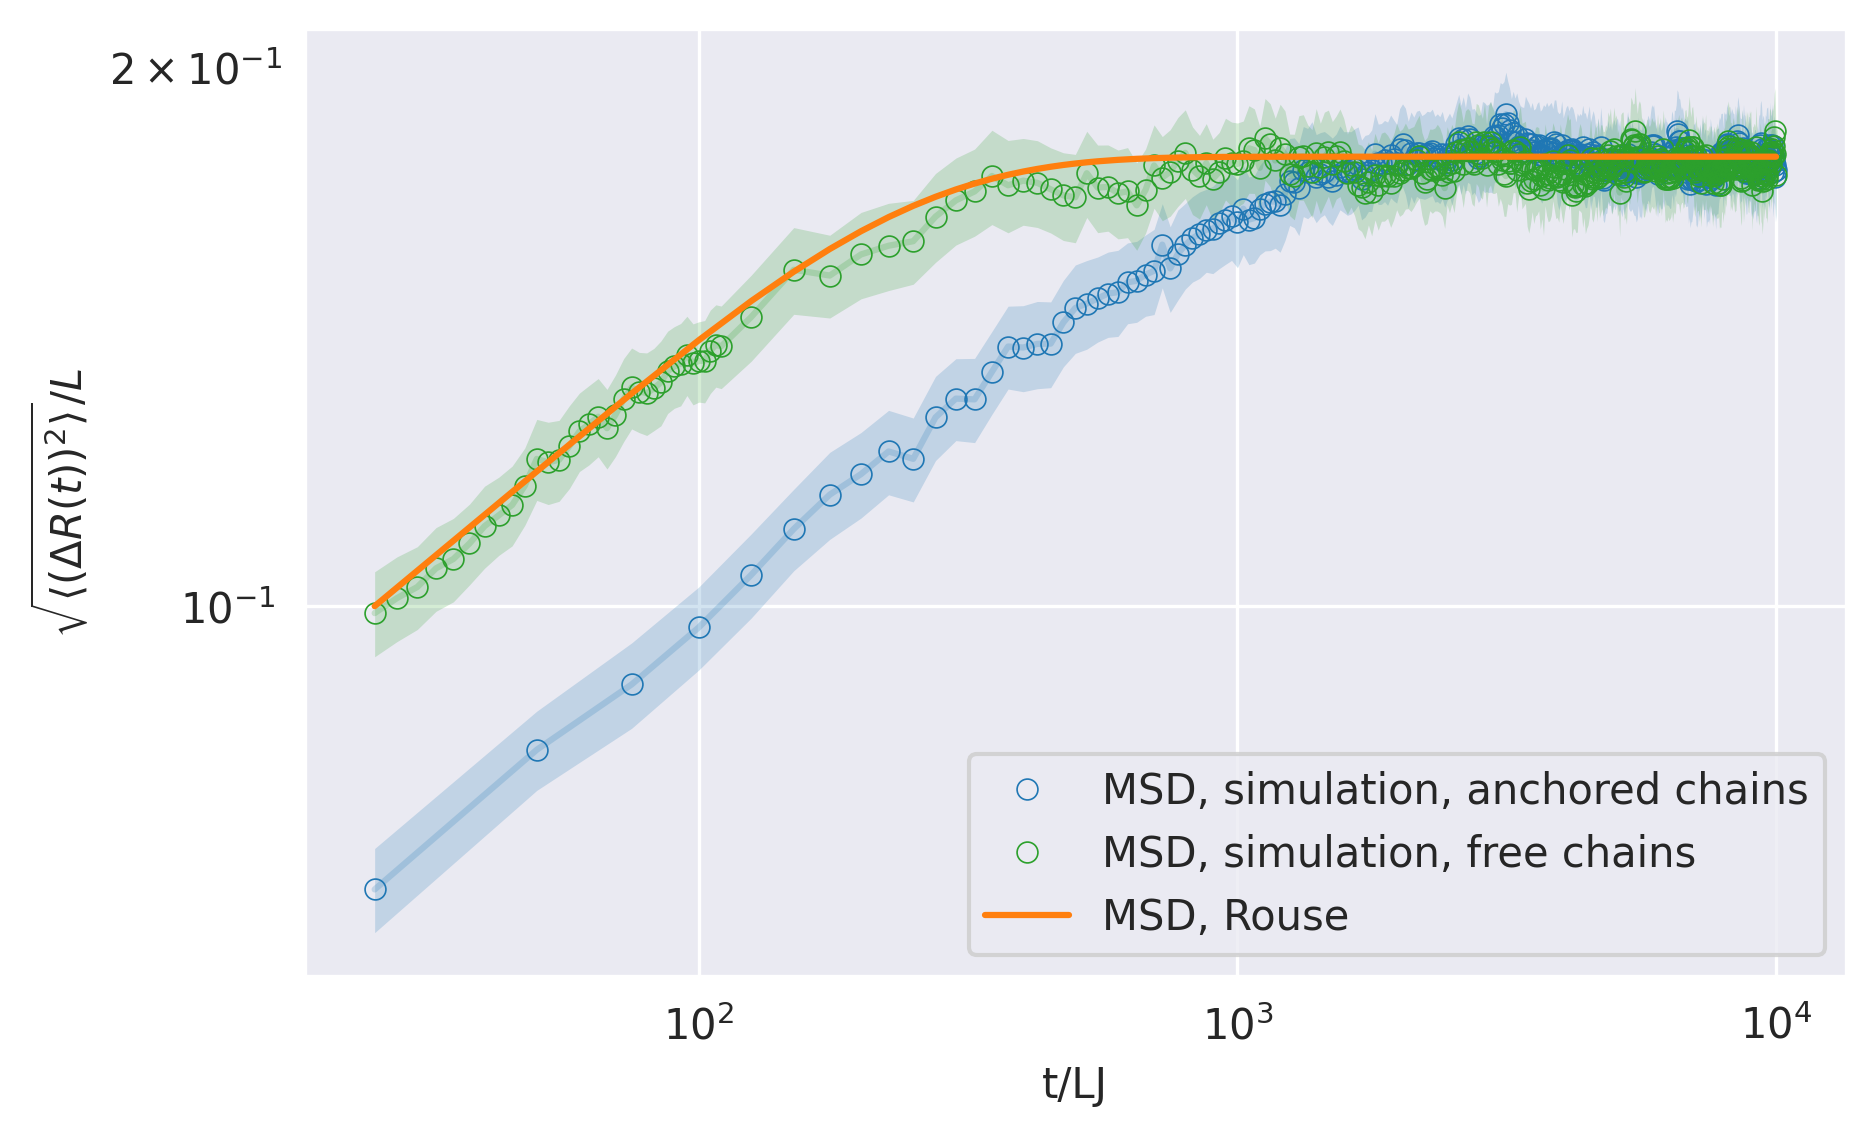
\includegraphics[width=\columnwidth,trim={0cm 0cm 0cm 0.9cm},clip]{3-exp-fixed-param-log.png}
      \caption{\label{fig:anchored_flex_chain_vs_rouse}
      MSD of ETE of an anchored fully flexible chain and
      MSD of ETE of a free fully flexible chain vs predictions of
      the analytical Rouse model (free chain, Eq. \ref{eq:rouse_msd_ete}).
      The filled area corresponds to the MSD curve $\pm$ 3 standard deviations of the mean. 
      The
      line connecting data points and the filled area between data points doesn't make
      any statements about probability of measuring values in this interval and is
      added for readability.
      }
    \end{center}
\end{figure}

\autoref{fig:anchored_flex_chain_vs_rouse} shows, that by anchoring the chain
the transition into a plateau is shifted to the right, increasing the 
relaxation time (Eq. \ref{eq:rouse_relaxation_time}), 
however the scaling behavior is visually the same. The Rouse relaxation time
of the free chain predicted using the Rouse model 
(with the same parameters as in the simulation, Section \ref{sec:simulation_setup})
is: $\tau_R=130.16$ (Eq. \ref{eq:rouse_relaxation_time}), 
$\tau_0=0.941$ (Eq. \ref{eq:rouse_tau_0}).
The Rouse relaxation time of the anchored chain estimated 
using the fit of the Eq. \ref{eq:rouse_msd_ete} with $\tau_R$ as free parameter
to the MSD curve of acnhored chain is: 
$\tau_R=555 \pm 62$, $\tau_0=4.1 \pm 0.5$, which is approximately $4$ times
larger. One needs to take into account, that the bond potential used in the simulations, 
FENE (Eq. \ref{eq:bond_potential}), does not match the bond potential 
used in the Rouse model, harmonic spring potential. Therefore, it is also 
necessary to compare the above mentioned results with the simulation of the free chain.
On the \autoref{fig:anchored_flex_chain_vs_rouse} is shown, that the predictions
of the Rouse model match the the resuts of the simulation of the free chains within the
confidence interval. The Rouse relaxation time of the free chain, estimated 
using the fit of the Eq. \ref{eq:rouse_msd_ete} with $\tau_R$ as free parameter
to the MSD curve of free chain is $\tau_R=138.6 \pm 14.3$, $\tau_0=1.0 \pm 0.1$,
which matches, within the confidence interval, the one analytically calculated.
The usage of $\tau_R$ as free parameter relies on the assumption, that
the dynamics of anchored chain obeys the same equations as dynamics of free chain, 
but with different time scales. The fitted curve is displayed on
\autoref{fig:anchored_flex_chain_vs_rouse_fitted}. The match of 
the fitted curve to the simulation data indirectly verifies this assumption.
Intuitively such difference is clear, the beginning of the anchored chain
can't move and therefore the chain needs more time to achieve the MSD limit, which
in case of fully flexible free chain is $2Nl_b^2$ as the one can see from Eq. \ref{eq:rouse_msd_ete}. 


\begin{figure}[h]
    \begin{center}
      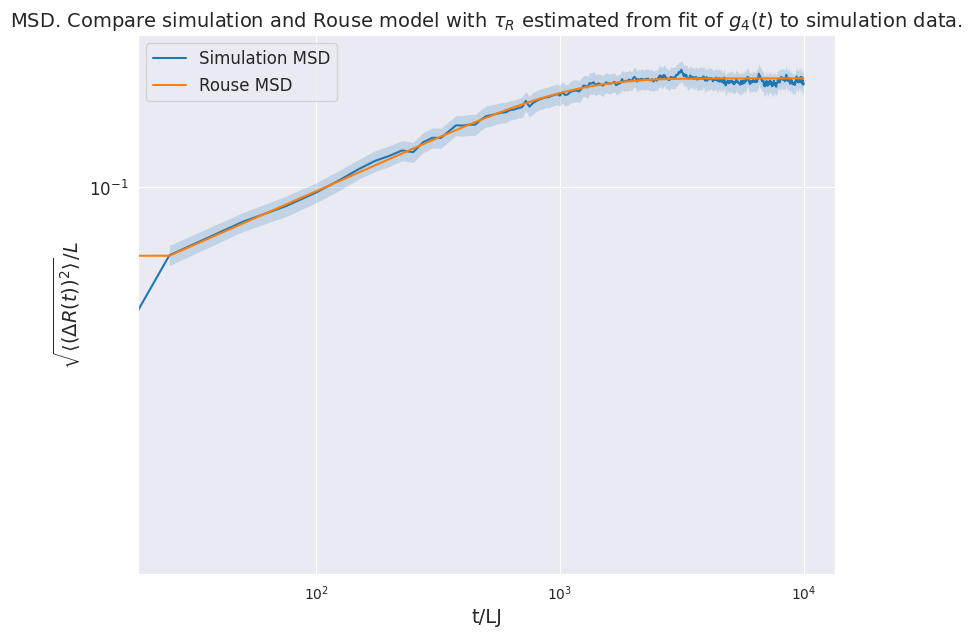
\includegraphics[width=\columnwidth,trim={0cm 0cm 0cm 0.8cm},clip]{3-exp-free-param-log.png}
      \caption{\label{fig:anchored_flex_chain_vs_rouse_fitted}
      MSD of ETE of an anchored fully flexible chain (blue points) and 
      MSD of ETE of a free fully flexible chain (green points).
      Fit of the modified 
      rouse model prediction 
      (Eq. \ref{eq:rouse_msd_ete}) with $\tau_R$ as a free parameter to the 
      MSD of ETE of an anchored fully flexible chain (grey line) and 
      to the MSD of ETE of a free fully flexible chain (purple line).
      The filled area corresponds to the MSD curve $\pm$ 
      3 standard deviations of the mean. The
      blue line connecting data points and the filled area between data points doesn't make
      any statements about probability of measuring values in this interval and is
      added for readability.
      }
    \end{center}
\end{figure}

It is possible to introduce correction factor based on the estimated $\tau_R$
to account for the boundary conditions:
\begin{equation}
    \label{eq:adj_factor_beta}
    \beta := \frac{\tau_{0, \textrm{simulation,anchored}}}{\tau_{0, \textrm{analytical, free}}} \approx 4.26
\end{equation}
\\
In this section predictions of the analytical Rouse model for 
the free fully flexible chains were compared to the data obtained 
from the simulation of the anchored fully flexible chains.
It has been found, that analytical Rouse model predictions of the MSD of the 
free fully flexible chain (Eq. \ref{eq:rouse_msd_ete}) can describe the 
anchored chain, if $\tau_R$ is considered as free parameter. However, we note,
that the predictions for anchored fully flexible chains can probably 
be obtained analytically by solving the Rouse model within the anchored boundary conditions 
(Eq. \ref{eq:rouse_boundary_anchored}) and the predictions obtained using the 
fit are not equivalent to the predictions derived analytically.
The comparison of 
analytically calculated $\tau_R$ (Eq. \ref{eq:rouse_relaxation_time}) of the free chain
with estimated $\tau_R$ of the anchored chain revealed, that 
$\tau_R$ of the anchored chain is significantly (4 times) larger. Finally, the
correction factor $\beta$ for $\tau_0$ was introduced to account for anchoring.

\FloatBarrier


\subsubsection{Impact of chain stiffness} \label{sec:impact_of_chain_stiffness}
Within this subsection, the focus shifts 
toward exploring the influence of chain stiffness on
the dynamics of anchored chains. 
By manipulating the angle potential (Eq. \ref{eq:angle_potential})
the MSD curves for different values
of the Kuhn length $l_K$ were measured. 
The analysis provides insights into 
how varying the chain stiffness exert an influence on the 
dynamics exhibited by anchored chain.
\autoref{table:kappa_values} shows the range of stiffness values examined
in this set simulations.
\\
\\
The MSD curves are plotted in \autoref{fig:msd_anchored_l_K} and the logarithmic
representation is given in \autoref{fig:msd_anchored_l_K_log}.
The following observations are made:
\begin{itemize}
    \item The relaxation time grows non-linearly with increasing $l_K$
    \item The long time MSD limit grows non-linearly with increasing $l_K$,
    however for $l_K/L >= 0.65$ it is not possible to distinguish 
    the curves any more because of the uncertainty.
\end{itemize}

\begin{figure}
    \centering
    \begin{subfigure}[b]{\textwidth}
        \centering
        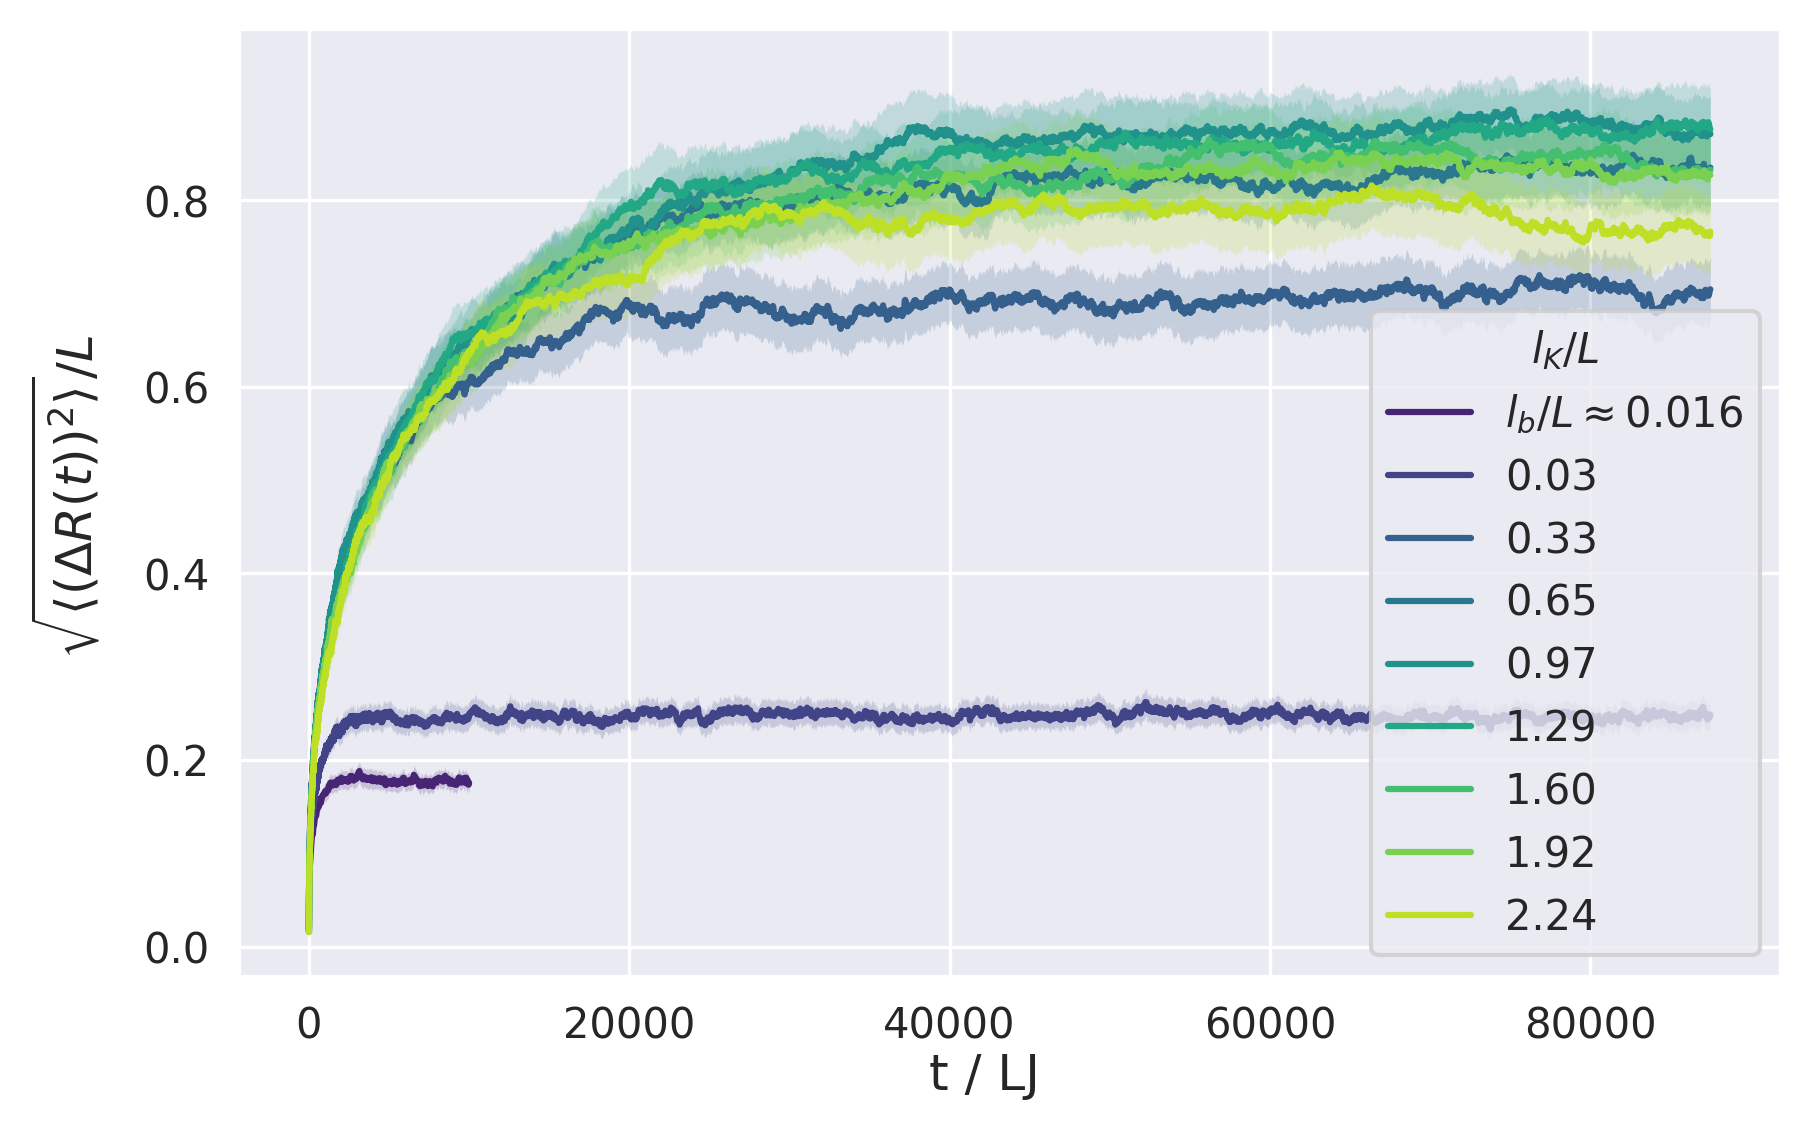
\includegraphics[width=\columnwidth,trim={0cm 0cm 0cm 0.0cm},clip]{4-exp-delta_R-bare.png}
        \caption{\label{fig:msd_anchored_l_K_normal}
        linear scale
        }
    \end{subfigure}
    \begin{subfigure}[b]{\textwidth}
        \centering
        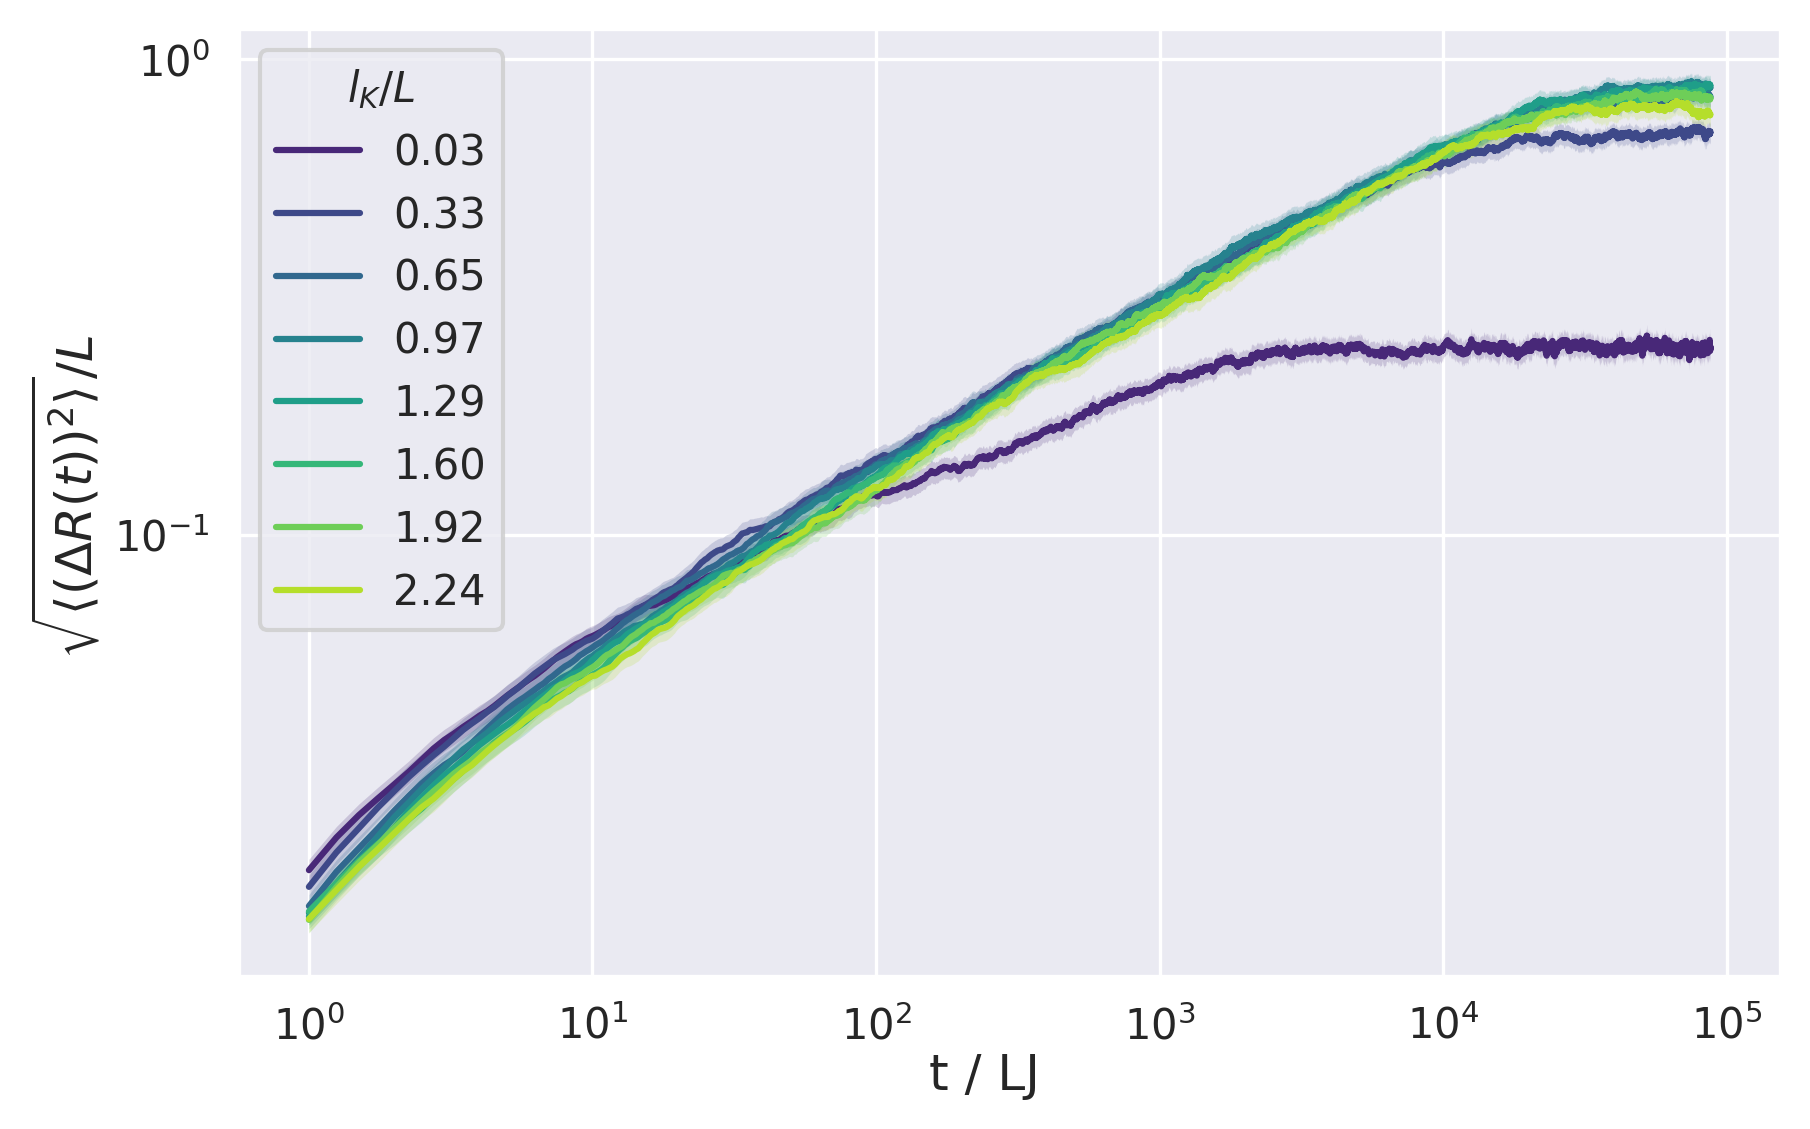
\includegraphics[width=\columnwidth,trim={0cm 0cm 0cm 0.0cm},clip]{4-exp-delta_R-bare-log.png}
        \caption{\label{fig:msd_anchored_l_K_log}
        log scale
        }
    \end{subfigure}
    \caption{Empirical MSD of ETE of anchored chains with different Kuhn length values.
    Filled area corresponds MSD curve $\pm$ 3 standard deviations of the mean.}
    \label{fig:msd_anchored_l_K}
\end{figure}

\begin{table}
    
    \centering
    \begin{tabular}{rrr}
        \toprule
        $\kappa$ & $N_K$ & $l_K/L$ \\
        \midrule
        0.00 & 63.00 & $l_b/L \approx 0.016$  \\
        1.00 & 32.96 & 0.03 \\
        11.00 & 3.00 & 0.33 \\
        21.00 & 1.54 & 0.65 \\
        31.00 & 1.03 & 0.97 \\
        41.00 & 0.78 & 1.29 \\
        51.00 & 0.62 & 1.60 \\
        61.00 & 0.52 & 1.92 \\
        71.00 & 0.45 & 2.24 \\
        \bottomrule
        \end{tabular}
    \caption{
        Values of $\kappa$ and corresponding $l_K$ tried in the study
        of anchored chain dynamics. Contour length $L=61.11$.
        }
    \label{table:kappa_values}
\end{table}

\FloatBarrier

\paragraph{Comparison with the Rouse model predictions for flexible chains}

Further, the empirical results are compared to the predictions of the Rouse model.
Firstly, the empirical results are compared to the Rouse model predictions for the fully
flexible chain with $N_K$ segments of length $l_K$. The results of this comparison are shown
in \autoref{fig:msd_anchored_l_K_rouse_fit_anal}. Then the empirical 
results are compared to the Rouse model predictions for fully flexible chain 
with $\tau_R$ as free parameter. The results of this comparison
are displayed in \autoref{fig:msd_anchored_l_K_rouse_fit-tau}. It is clear, 
that the Rouse model predictions for fully flexible chain doesn't match
the observed behavior of semiflexible anchored chains even with $\tau_R$ as 
free parameter. This result matches the intuition, that deviations from  
the Rouse model predictions for the free, fully flexible chains increase 
with increasing $l_K$, because semiflexible chains require separate and more complicated
description (section \ref{sec:rouse_semiflex_chain}), 
than the fully flexible ones within the Rouse model.


\begin{figure}
    \begin{center}
      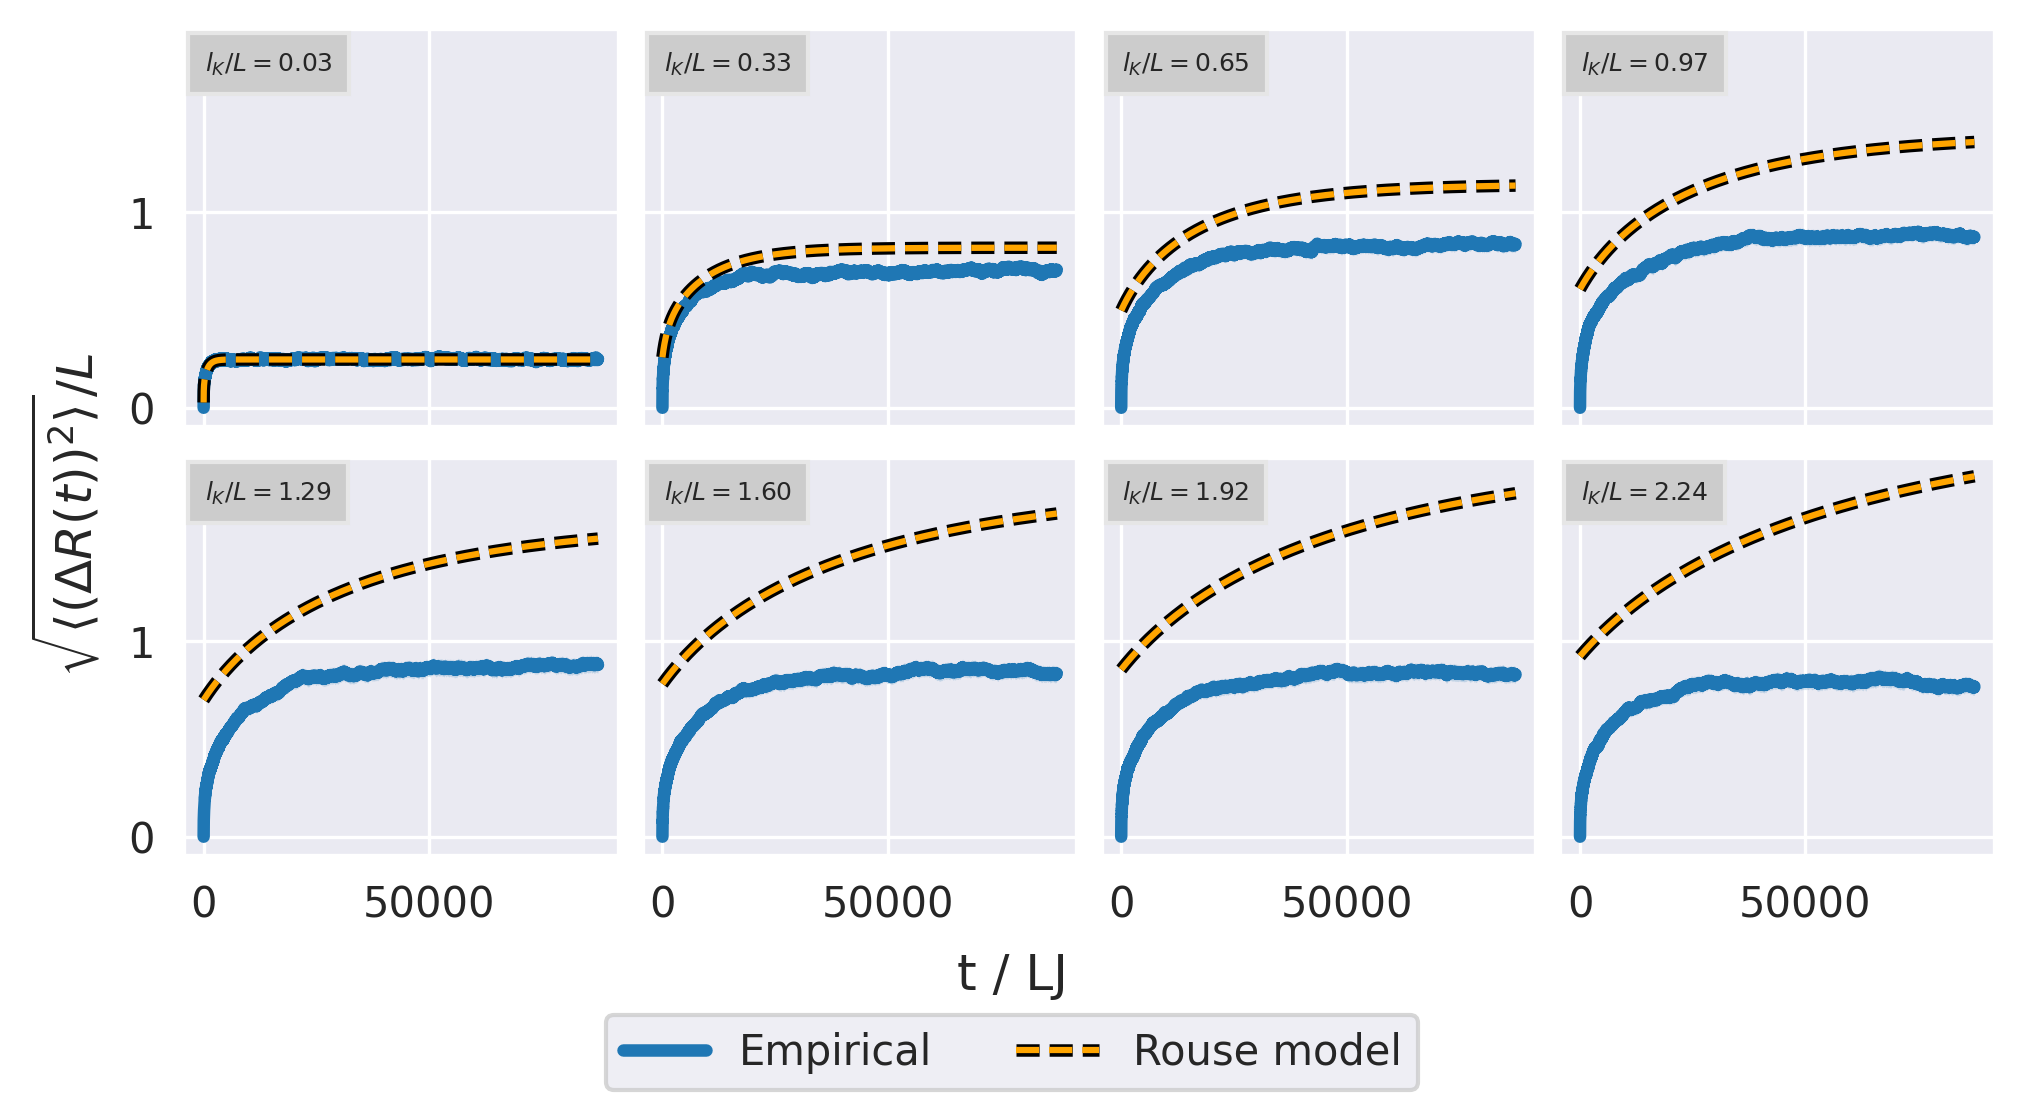
\includegraphics[width=\columnwidth,trim={0cm 0cm 0cm 0.0cm},clip]{4-exp-delta_R-rouse_anal.png}
      \caption{\label{fig:msd_anchored_l_K_rouse_fit_anal}
      Empirical MSD of ETE of anchored chains with different Kuhn length values
      and Rouse model prediction for fully-flexible chains (Eq.\ref{eq:rouse_msd_ete})
      with $N_b = N_K$ if $N_K \ge 1$ or $N_b=1$ otherwise. $\tau_R$ adjusted
      using $\beta$ (Eq.\ref{eq:adj_factor_beta}) to account for boundary conditions.
      }
    \end{center}
\end{figure}
\begin{figure}
    \begin{center}
      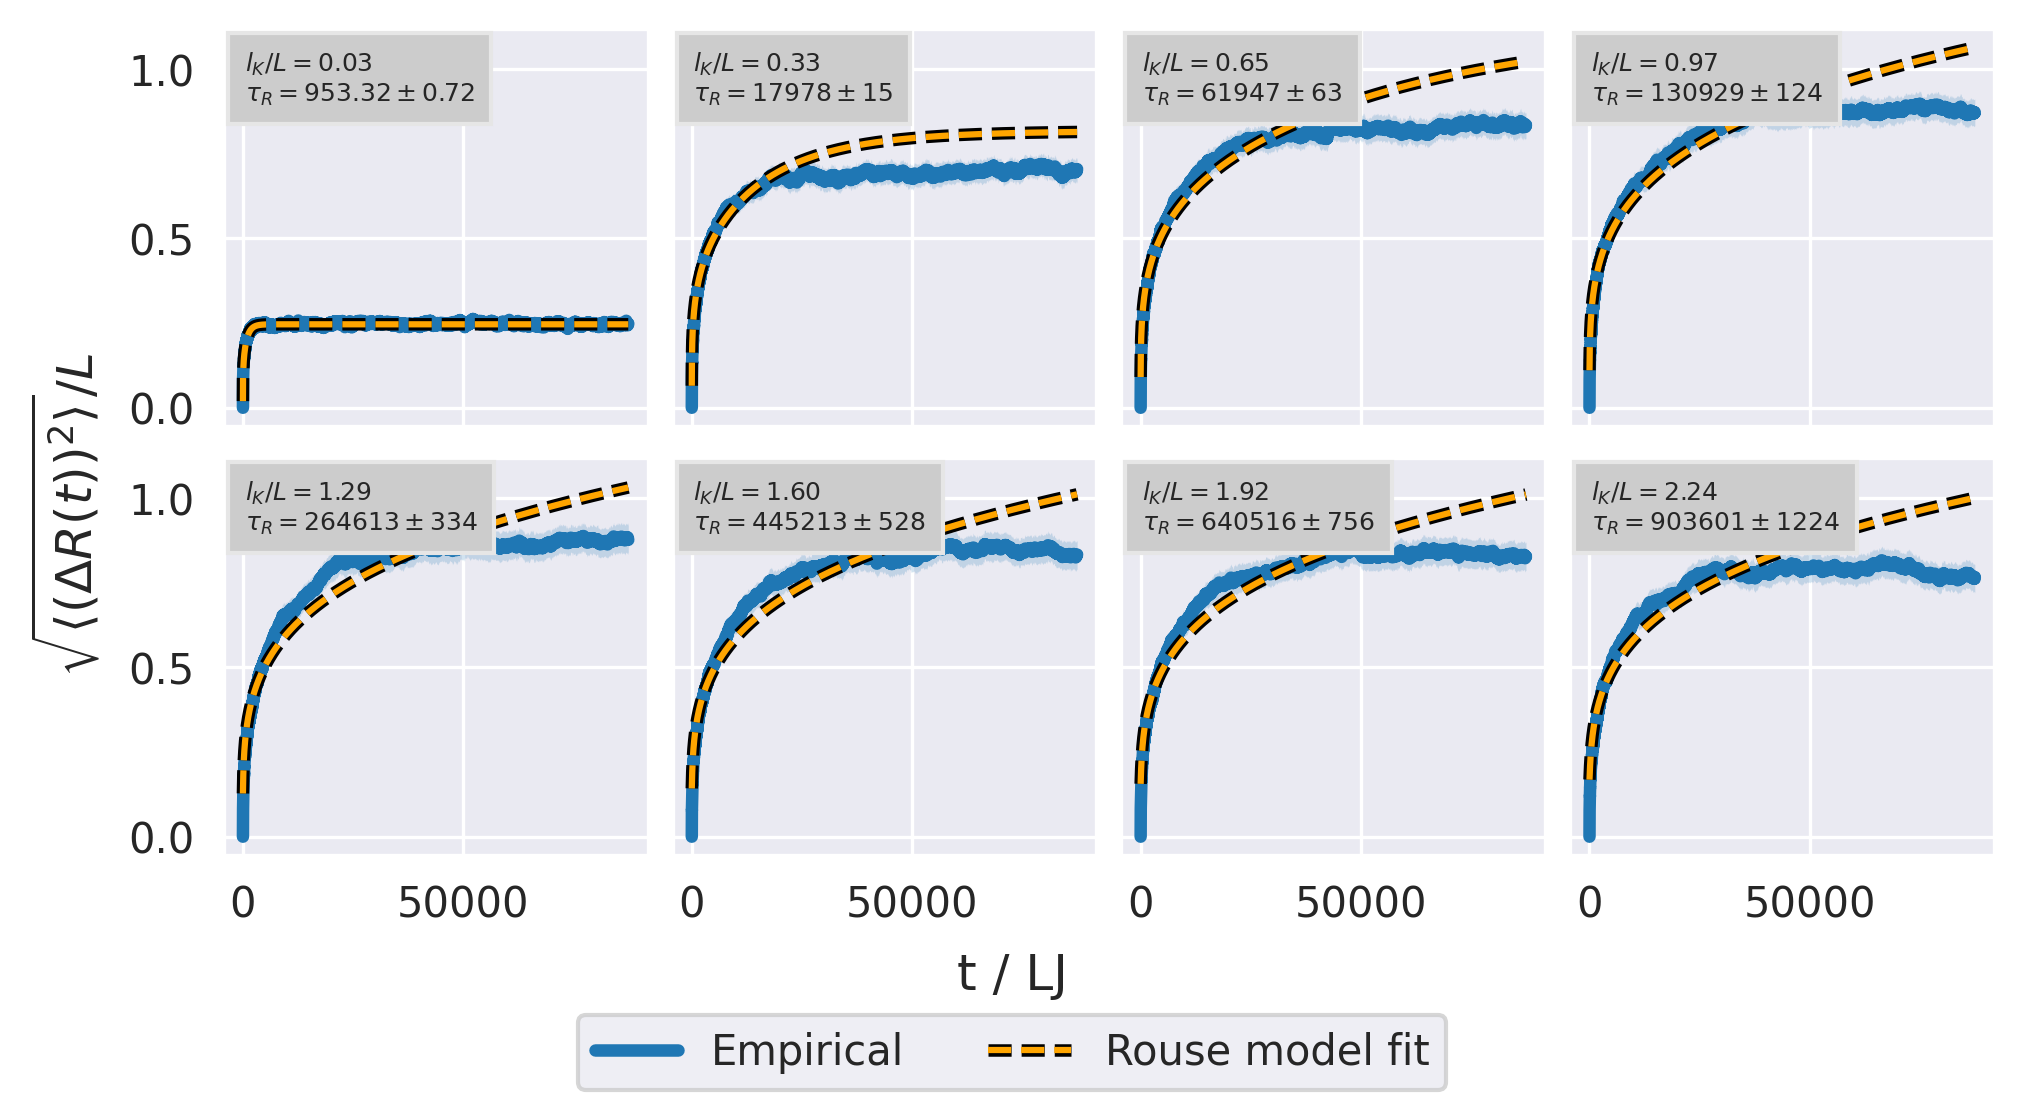
\includegraphics[width=\columnwidth,trim={0cm 0cm 0cm 0.0cm},clip]{4-exp-delta_R-rouse_fit-tau.png}
      \caption{\label{fig:msd_anchored_l_K_rouse_fit-tau}
      Empirical MSD of ETE of anchored chains with different Kuhn length values
      and fit of Rouse model prediction for fully-flexible chains 
      (Eq.\ref{eq:rouse_msd_ete}) with $N_b = N_K$ if $N_K \ge 1$ or $N_b=1$ otherwise.
      $\tau_R$ is free parameter. The summation in Eq.\ref{eq:rouse_msd_ete}
      does not extend to $N_K$ as it should strictly do, but up to the number of bonds (63)
      of the fully flexible chain.
      }
    \end{center}
\end{figure}

\FloatBarrier

\paragraph{Comparison with Rouse model predictions for semiflexible chains}
\label{sec:comp_with_rouse_semiflex}

Furthermore, the empirical MSD curves are compared to the predictions
of the Rouse model for the semiflexible chains. The autocorrelation function
of the End-to-End vector was already discussed in Section \ref{sec:rouse_semiflex_chain}.
The MSD can be written as 
$$\E{[\Delta \vec{R}(t)]^2} = \E{R^2(t)} - 2 \E{\vec{R}(t)\vec{R}(0)} + \E{R^2(0)} = 2(\E{R^2} - \E{\vec{R}(t)\vec{R}(0)})$$
where the term $\E{\vec{R}(t)\vec{R}(0)}$ in case of free semiflexible chain obeys 
the relationships discussed in Section \ref{sec:rouse_semiflex_chain}.

To compare the long time case with empirical results, the expression
$2(\E{R^2} - k \exp(-t/\tau_{rot}))$ with $k$ as free paramater was fitted 
to the part of the corresponding empirical MSD curves as specified in 
Eq. \ref{eq:autocorr_ete_coil_limit_long_time} and Eq. \ref{eq:autocorr_ete_rod_limit}.
The result was then visually examined against the empirical curve.
This comparison revealed, that MSD in long time limit based on 
Eq. \ref{eq:autocorr_ete_coil_limit_long_time} and 
Eq. \ref{eq:autocorr_ete_rod_limit} does not correspond to the empirical curves.
However, an introduction of two meaningful free parameters 
($a$, $\tau_{rot}$) is able to dismiss
the discrepancy between theoretical approach for the free chain and empirical 
results for the anchored chain:
\begin{equation}
    \label{eq:adjusted_rouse_model_ete}
    \E{[\Delta \vec{R}(t)]^2}  = a\E{R^2}\left[1 - \exp\left(-\frac{t}{\tau_{rot}}\right)\right]
\end{equation}
This equation is referred further as "Adjusted Rouse model".
The free parameter $a$ accounts the for large-time limit of MSD and $\tau_{rot}$ 
accounts for the location of the transition into the plateau. However, one
can only speculate, whether the new $\tau_{rot}$ has the same meaning
as the old one. The results of this fit are shown in 
\autoref{fig:msd_anchored_l_K_rouse_fit_tau-a}.
It is possible to conclude, that in case of anchored chains the proportionality
$\E{\vec{R}(t)\vec{R}(0)} \propto \exp(-\frac{t}{\tau_{rot}})$
holds for $t>\tau_{rot}$ but with a different value (and eventually meaning) of $\tau_{rot}$.
In case of the chains close to the rod-limit one can see that in analogy with 
the case of free chains in the rod limit there should be some analogy of 
characteristic time $\tau_1$ (from Eq. \ref{eq:autocorr_ete_rod_limit}), which 
is smaller than the simulated $\tau_{rot}$, and where the above mentioned 
proportionality starts to be valid.

\begin{figure}
    \centering
    \begin{subfigure}[b]{\textwidth}
        \centering
        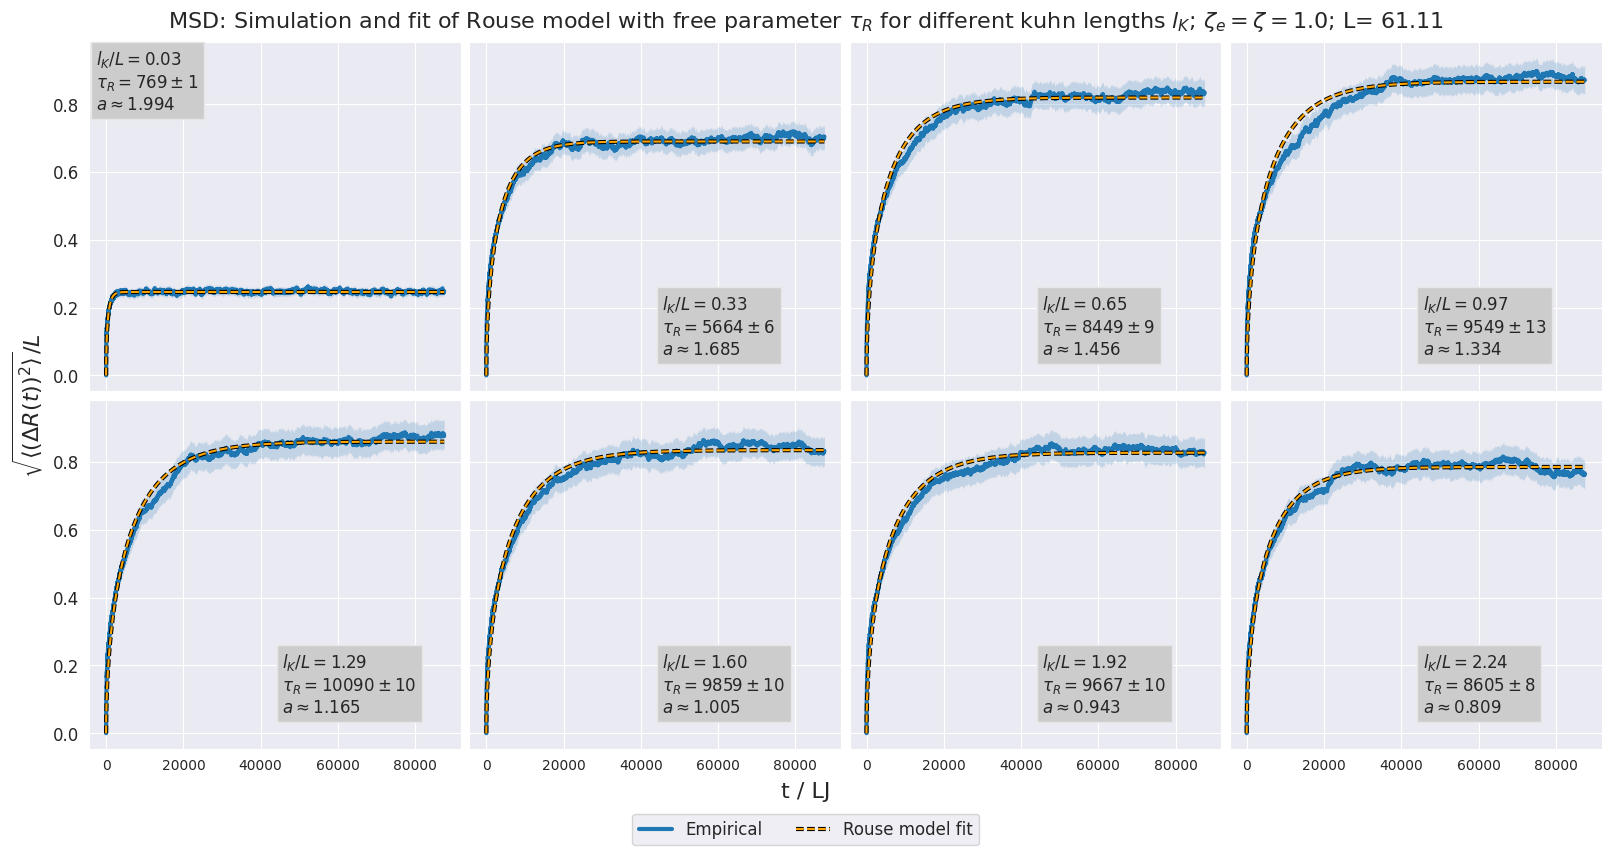
\includegraphics[width=\textwidth]{4-exp-delta_R-rouse_fit-tau-a.png}
        \caption{linear scale}
        \label{fig:msd_anchored_l_K_rouse_fit_tau-a_normal}
    \end{subfigure}
    \begin{subfigure}[b]{\textwidth}
        \centering
        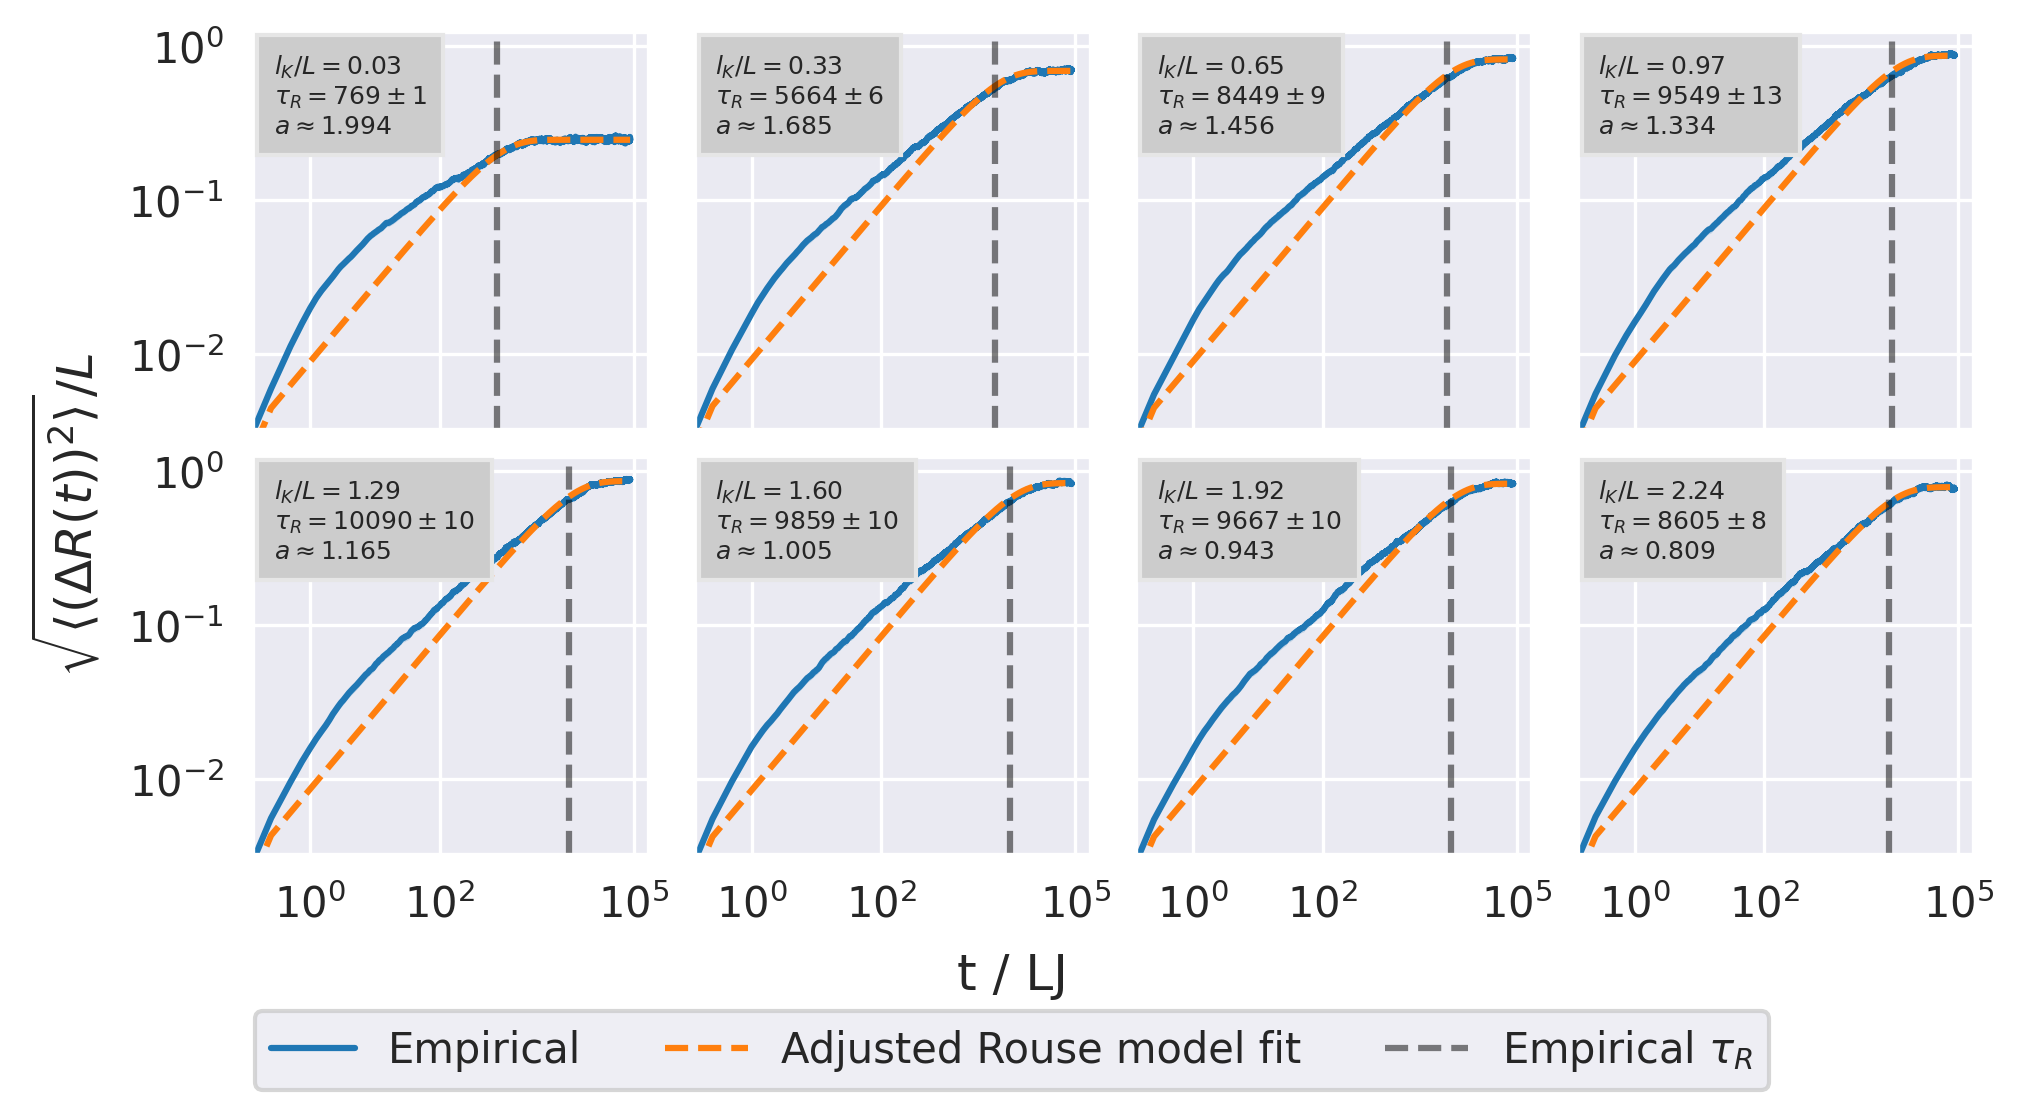
\includegraphics[width=\textwidth]{4-exp-delta_R-rouse_fit-tau-a_log.png}
        \caption{log-log scale}
        \label{fig:msd_anchored_l_K_rouse_fit_tau-a_log}
    \end{subfigure}
    \caption{Empirical MSD of ETE of anchored chains with different Kuhn length values 
    (blue line),
    and fit of the modified Rouse model prediction for semiflexible chains 
    (Eq.\ref{eq:adjusted_rouse_model_ete}, dashed line) on log-log scale.
    Estimated (empirical) $\tau_{rot}$ is drawn as vertical dashed line.}
    \label{fig:msd_anchored_l_K_rouse_fit_tau-a}
\end{figure}

\vspace{0.5cm}
Further, the case of short times is examined. To execute this comparison,
the scaling behavior of the empirical MSD is analyzed. It is clear, that
$\E{[\Delta \vec{R}(t)]^2} \propto t^{\alpha(t)}$ for the small times is valid
in analogy to the scaling behavior of MSD of the last monomer of the free chain. 
The scaling exponent $\alpha$ is estimated from the MSD curves as 
described in Section \ref{sec:est-alpha-msd} with $n=10$ bins. 
The result is shown on \autoref{fig:alpha_anchored_l_K}.
Further in this paragraph $\alpha_{min}$ refers to the scaling exponent $\alpha$
in the region in which the overdamped motion takes place and $t \ll \tau_{rot}$. 
For the nearly flexible chain $l_K/L = 0.03$ $\alpha_{min} \approx \frac{1}{2}$
is observed, which matches theoretical expectations for fully flexible chain 
(section \ref{sec:rouse_flexible_chain}).
For semiflexible chains the value $\alpha_{min}$ is close to $\frac{3}{4}$, which
matches the scaling behavior of free chain at short times. 
One can see, that $\alpha_{min}$ gets closer to $\frac{3}{4}$ with rising $l_K$. Larger
scaling factor in the region $[1, 10]$ is due to transition from 
ballistic motion at time scales $t<\frac{1}{\sigma} = 1$ to the overdamped motion.
Additionaly, $\alpha$ for $t>\tau_{rot}$ matches the one of rouse model prediction
for free semiflexible chain as well as $\alpha$ transitions in this regime smoothly
near the $\tau_{rot}$.

\begin{figure}[h]
    \begin{center}
      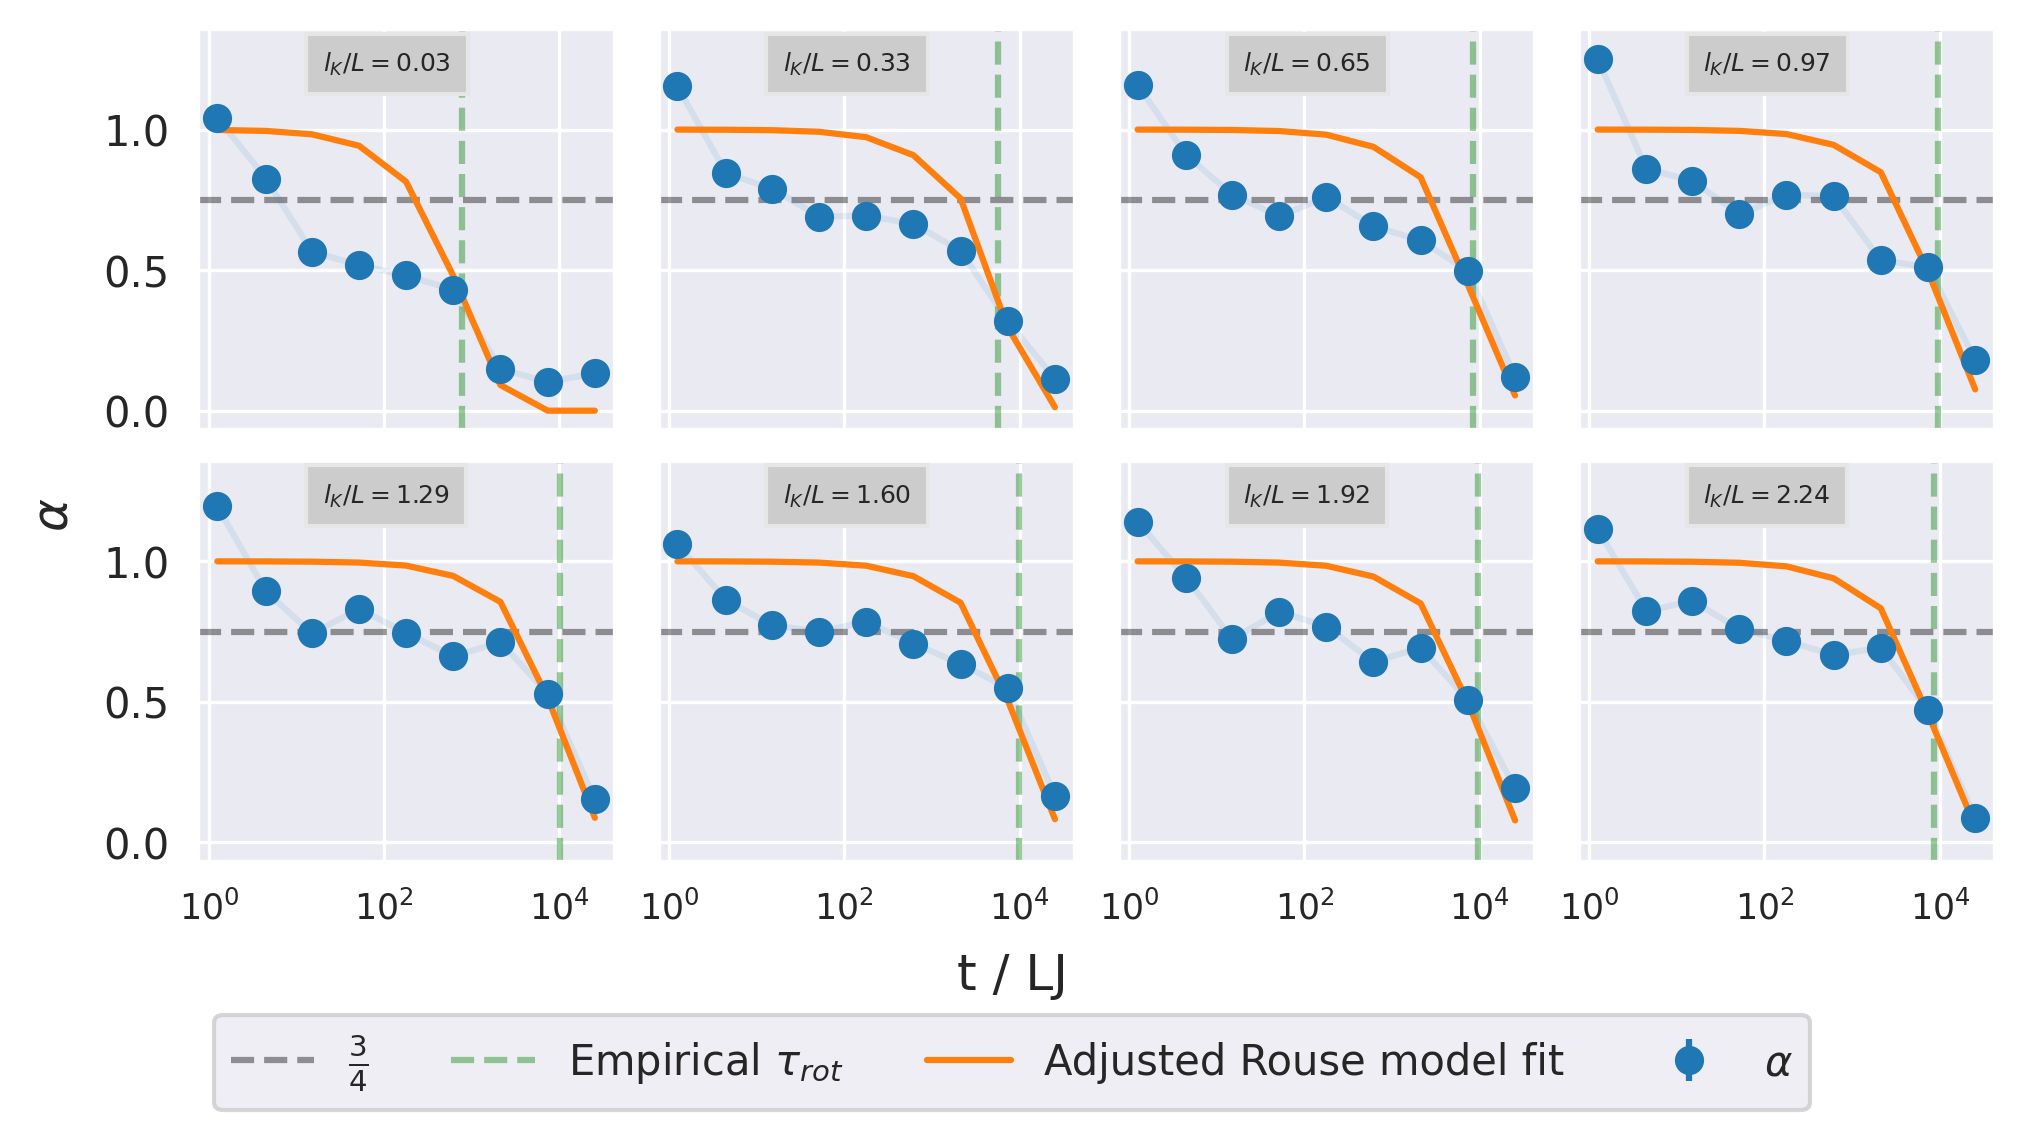
\includegraphics[width=\columnwidth,trim={0cm 0cm 0cm 0.0cm},clip]{4-exp-delta_R-rouse_fit-tau-a_alpha.png}
      \caption{\label{fig:alpha_anchored_l_K}
      Scaling exponent $\alpha$ of the MSD of ETE of anchored semiflexible chain (blue points) and 
      scaling exponent $\alpha$ of the Adjusted Rouse model prediction for semi-flexible chains 
      (Eq.\ref{eq:adjusted_rouse_model_ete}, orange line).
      Estimated (empirical) $\tau_{rot}$ is drawn as vertical dashed line.
      Horizontal grey dashed line corresponds to $\frac{3}{4}$ value.
      Black line on the top left plot corresponds to the scaling exponent 
      $\alpha$ of the modified Rouse model prediction 
      (Eq. \ref{eq:rouse_msd_ete}
      with $\tau_R$ as free parameter, estimated in section \ref{sec:comp_to_free_chain},
      $\tau_R \approx 582.3$) for 
      for anchored flexible chains as explained in section \ref{sec:comp_to_free_chain}.
      }
    \end{center}
\end{figure}

\FloatBarrier


\paragraph{Separation of the dynamics into components parallel and perpendicular
to the main-axis}
Further, the MSD in main-axis coordinate system (section \ref{sec:main-axis}) is analyzed.
\autoref{fig:msd_anchored_l_K_by_dim} shows the MSD curves in main axis system
for each dimension. The analysis delivers following insights:
\begin{itemize}
    \item The difference of MSD in $z$ dimension relative to the $x$ and $y$
    dimensions rises with growing stiffness. The plateau value of MSD falls.
    \item The MSD in $z$ dimension has smaller relaxation time in case $l_K/L \ge 0.95$ 
\end{itemize}
The chain becomes more straight with rising stiffness and therefore has less
freedom of movement along the $z$ direction, which results in a smaller MSD and quicker
relaxation.

\begin{figure}
    \begin{center}
      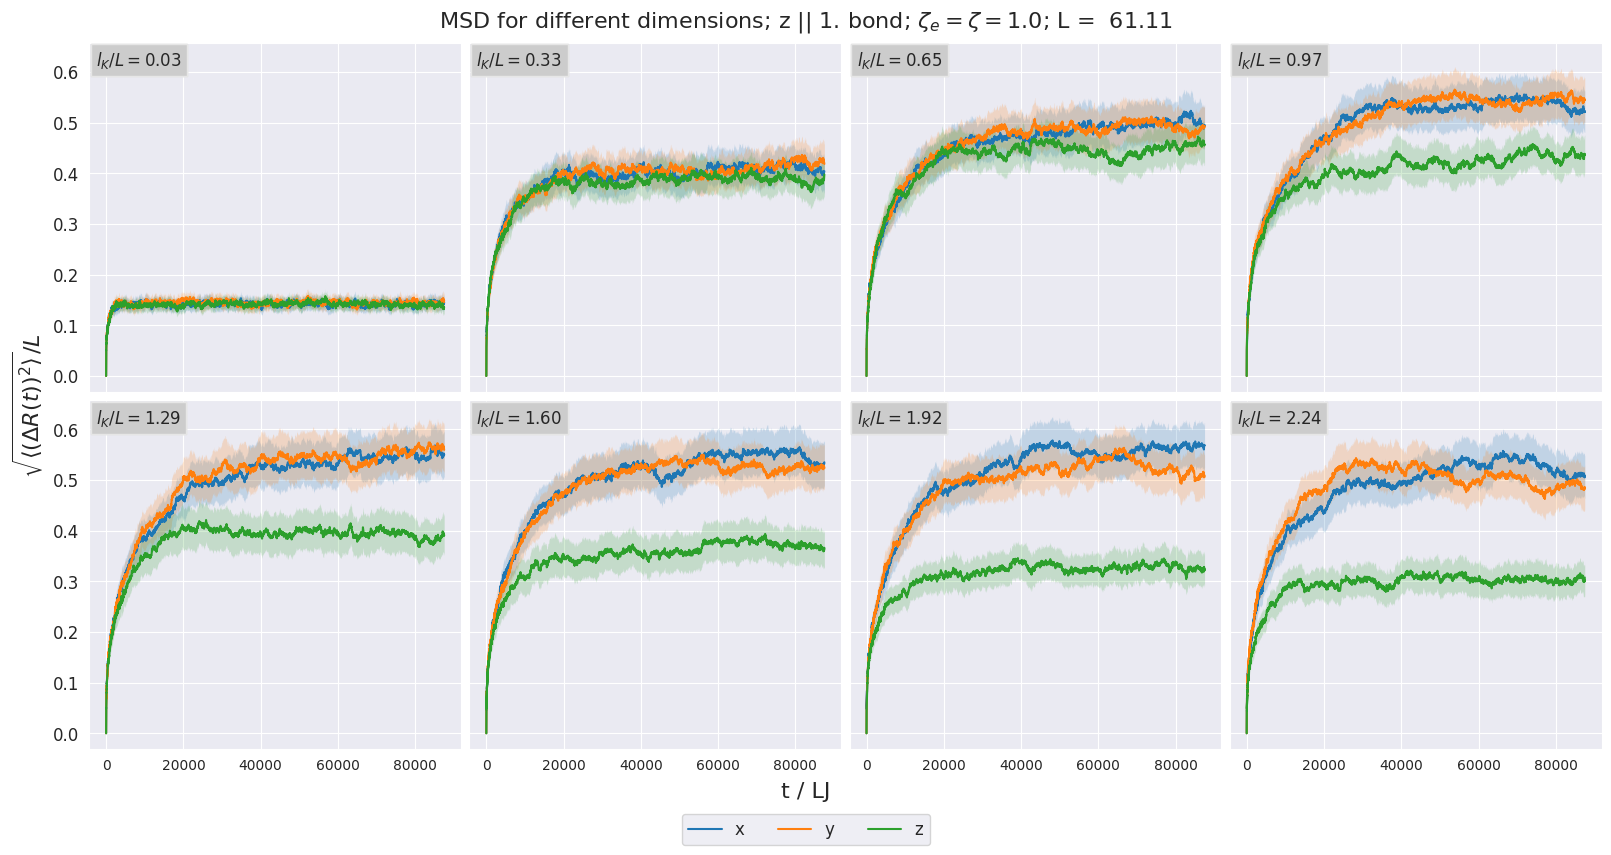
\includegraphics[width=\columnwidth,trim={0cm 0cm 0cm 0.0cm},clip]{4-exp-msd_by_dim.png}
      \caption{\label{fig:msd_anchored_l_K_by_dim}
      Empirical MSD of ETE of anchored chains with different Kuhn length values in
      main-axis coordinate system (See section \ref{sec:main-axis}). For reasons of
      the system's symmetry, the x and y components have to behave identically.
      }
    \end{center}
\end{figure}

\FloatBarrier

\subsubsection{Impact of the friction coefficient of the chain end}
\label{sec:impact_of_zeta_e}
In this subsection, the focus turns to the influence 
of the friction coefficient at the chain end on the dynamics of anchored chain with high
stiffness.
\\
\\
In the simulation this is achieved by changing the value of the damping constant 
of the Langevin thermostat
for the last bead of the chain. Assuming the Stokes friction, 
changing the value of the damping parameter effectively means a change of the 
bead diameter. The mass of the end bead is set to the $m_e = 1.5$ 
(a modification of the mass is arbitrary, 
but it affects the damping time $\tau_d=m_e/\zeta_e$)
and friction coefficient of end bead
is varied: $\zeta_e = 10, 15$, which corresponds to the end-bead diamaters: $15, 30$.
The reference value provides simulation of the chain with $\zeta_e=\zeta=1$ and $m_e=m=1$.
In all 3 cases $\kappa=190.2$, which results in Kuhn length $l_K/L=6.02$. The chosen
persistence length of the chains relative to their contour length $l_p/L=l_K/(2L)=3.01$ matches
the one of the unbound EEA1 \cite{Singh:2022}.

\paragraph{Comparison with the Rouse model}
The approach mostly follows section \ref{sec:impact_of_chain_stiffness} with an exception that
the friction coefficient of the chain end $\zeta_e$ is varied instead of Kuhn length $l_K$ 
of the chain. The resulting MSD curves are shown on 
\autoref{fig:msd_anchored_zeta}. Again, the adjusted Rouse model 
(Eq. \ref{eq:adjusted_rouse_model_ete}) is fitted to
the MSD curves (\autoref{fig:msd_anchored_zeta-arm_fit}). One can see
the perfect match on time scales $t > \tau_{rot}$. Also, the estimated $\tau_{rot}$
rise with rising $\zeta_e$ and the scaling behavior on short time scales 
varies. To investigate the scaling behavior, the scaling exponent $\alpha$ is
calculated as described in section \ref{sec:est-alpha-msd} 
within $n=20$ bins and is plotted on \autoref{fig:alpha_anchored_zeta}.
The Rouse model for semiflexible free chains predicts $\alpha=3/4$ on the
time scales $t < \tau_{1} \ll \tau_{rot}$. To test if this holds for chains with larger
friction coefficient of the chain end it's necessary to estimate $\alpha$ in this
region. We define $\alpha_m := \alpha \text{ for } t \ll \tau_{rot}$.
Based on \emph{Nikoubashman et. al.} \cite{Nikoubashman2016} finding,
that the crossover from ballistic motion to anomalous diffusion, as described 
in Rouse model, lasts 2 decades of time, it is assumed, 
that the left boundary of this region is given by the end of the region of the 
crossover from the ballistic
motion to the anomalous diffusion of the end bead, $\tau_b  := 10 \frac{m}{\zeta_e}$. 
The right boundary is
assumed to be $\tau_{rot} / 10$ to match $t \ll \tau_{rot}$ requirement.
The boundaries of the region are plotted as a red dashed line and vizually match
the observed scaling behavior. $\alpha_m$ is then calculated as the mean
of observed $\alpha$ in the region. The measurement uncertainty is estimated
as 3 standard deviations of the mean. All estimated quantities are summarized
in \autoref{table:anchored_chain_zeta_estimations}. One can see the 
small increase of $\alpha_m$ by transition from $\zeta_e=1$ to $\zeta_e=10$ and, 
given the confidence interval, there is no difference between 
$\alpha_m$ for $\zeta_e = 10$ and $\zeta_e=20$.

\paragraph{Separation of the dynamics into components parallel and perpendicular to
the main-axis}
Additionaly different dimensions of the MSD in main-axis coordinate system are
analyzed and the results are shown on \autoref{fig:msd_anchored_zeta-dim}.
One can observe, that the visual patterns of 
increasing $\zeta_e$ for all dimensions are the same.

\begin{figure}
    \centering
    \begin{subfigure}[b]{\textwidth}
        \centering
        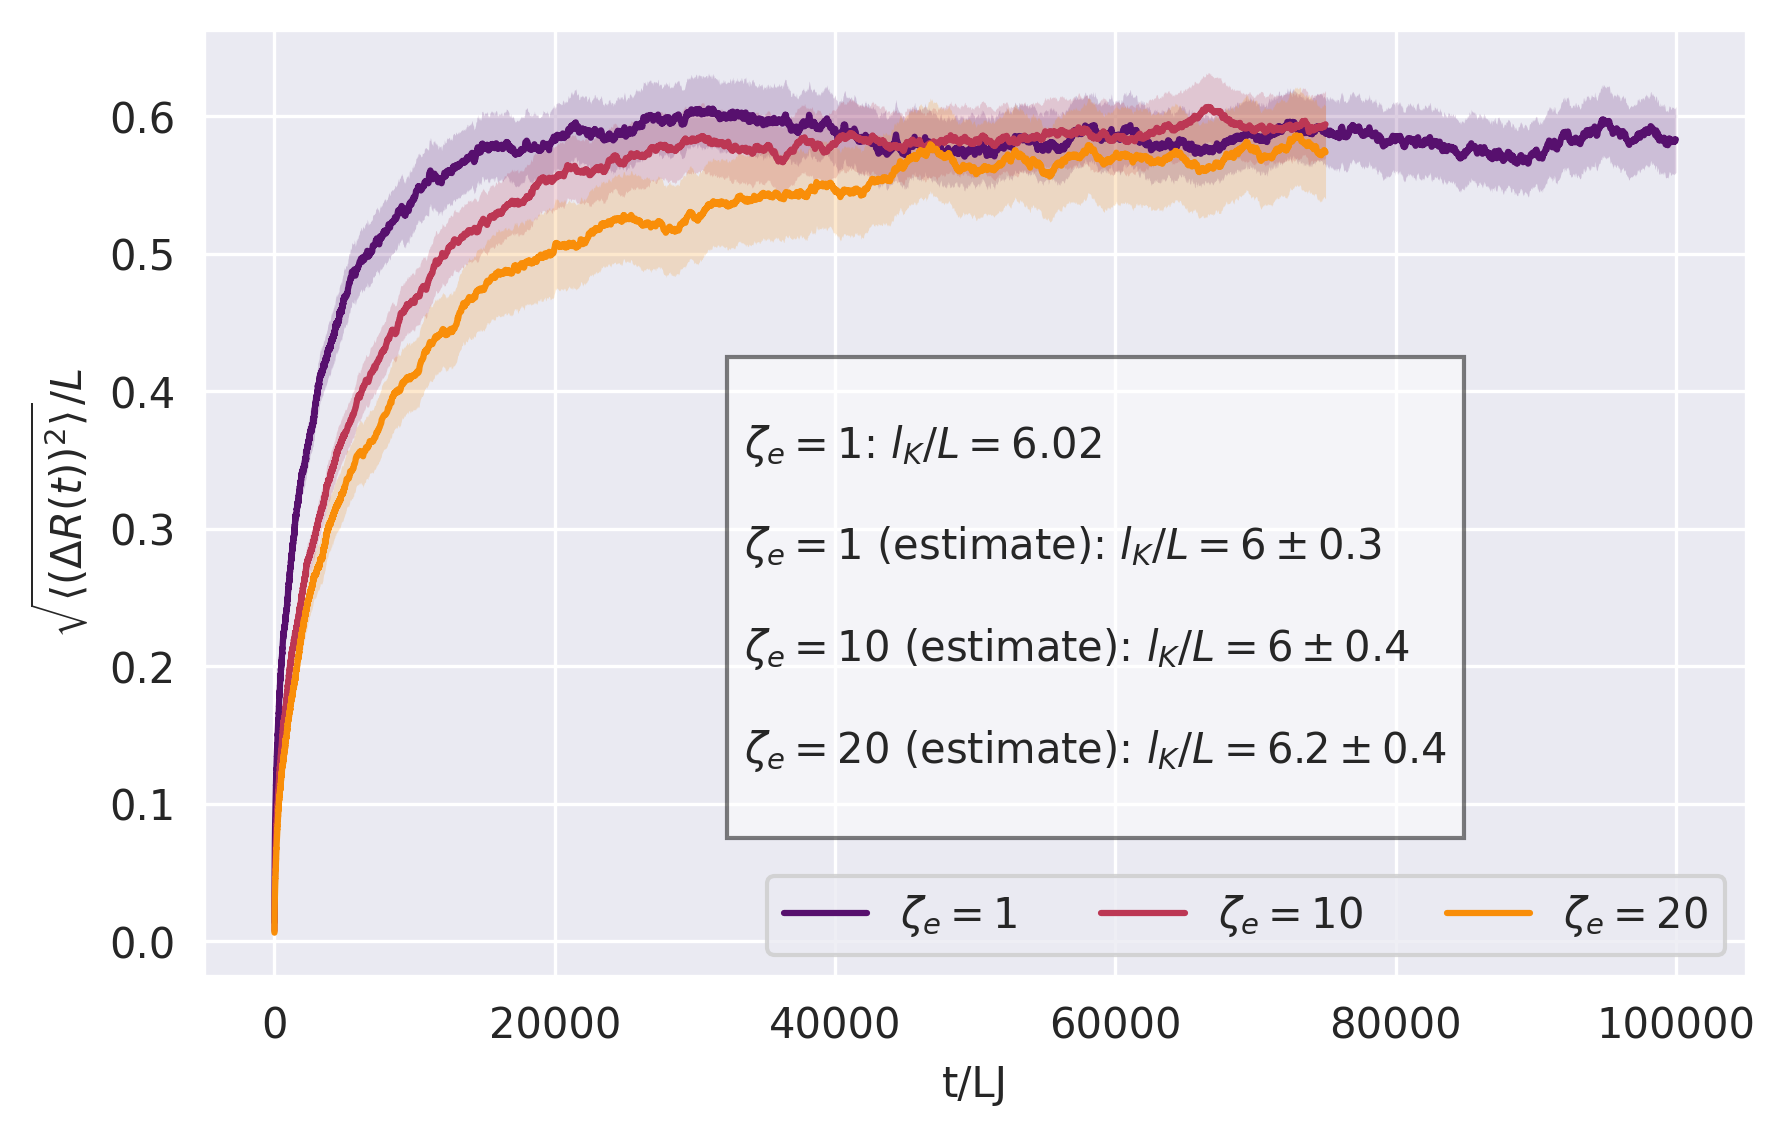
\includegraphics[width=\textwidth]{14+15+16-exp-msd.png}
        \caption{linear scale}
        \label{fig:msd_anchored_zeta-normal}
    \end{subfigure}
    \begin{subfigure}[b]{\textwidth}
        \centering
        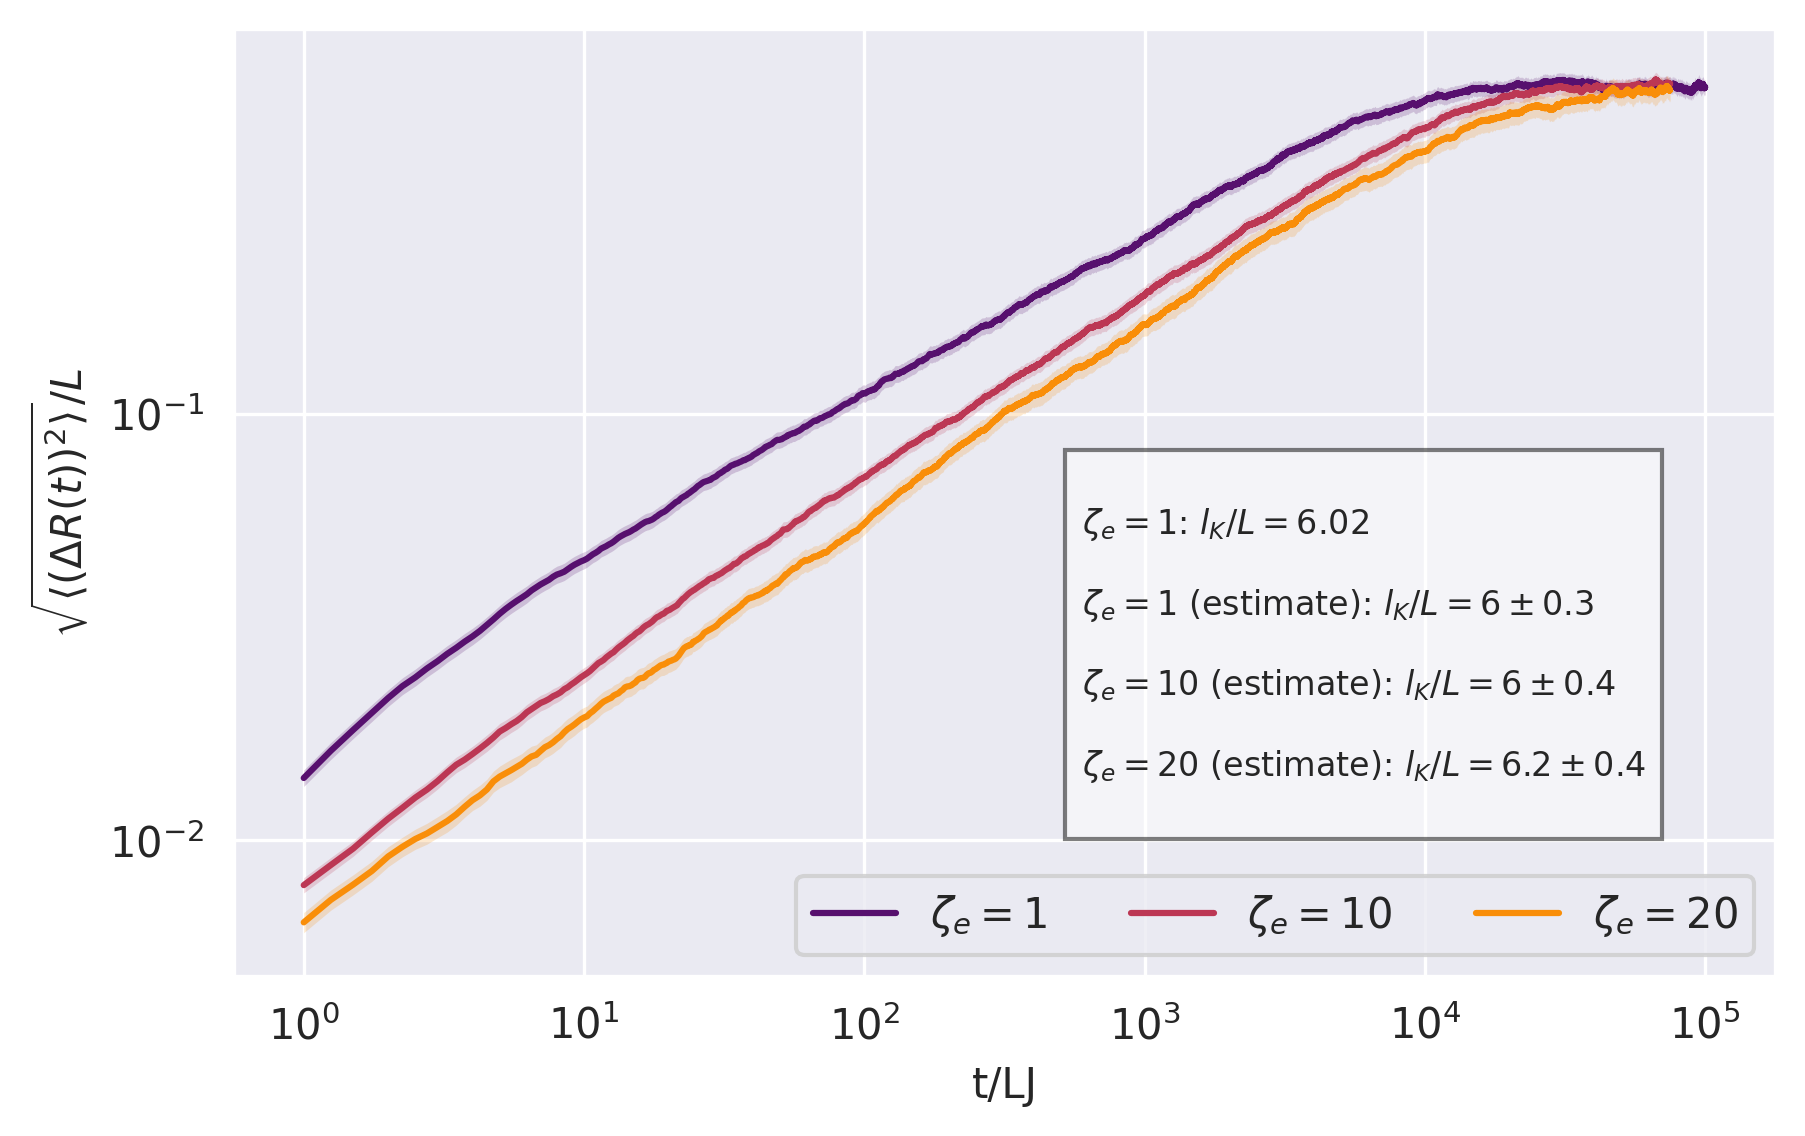
\includegraphics[width=\textwidth]{14+15+16-exp-msd-log.png}
        \caption{log-log scale}
        \label{fig:msd_anchored_zeta-log}
    \end{subfigure}
    \caption{Empirical MSD of ETE of anchored chains with different values of
    the friction coefficient of the chain end $\zeta_e$. 
    Configured and estimated Kuhn length is shown in the text box (as
    additional check of plausibility).
    An estimate of the Kuhn length is done using a fit of 
    \autoref{eq:worm-like-chain-cos-theta-ij} with $l_p$ as free parameter.
    }
    \label{fig:msd_anchored_zeta}
\end{figure}

\begin{figure}
    \centering
    \begin{subfigure}[b]{\textwidth}
        \centering
        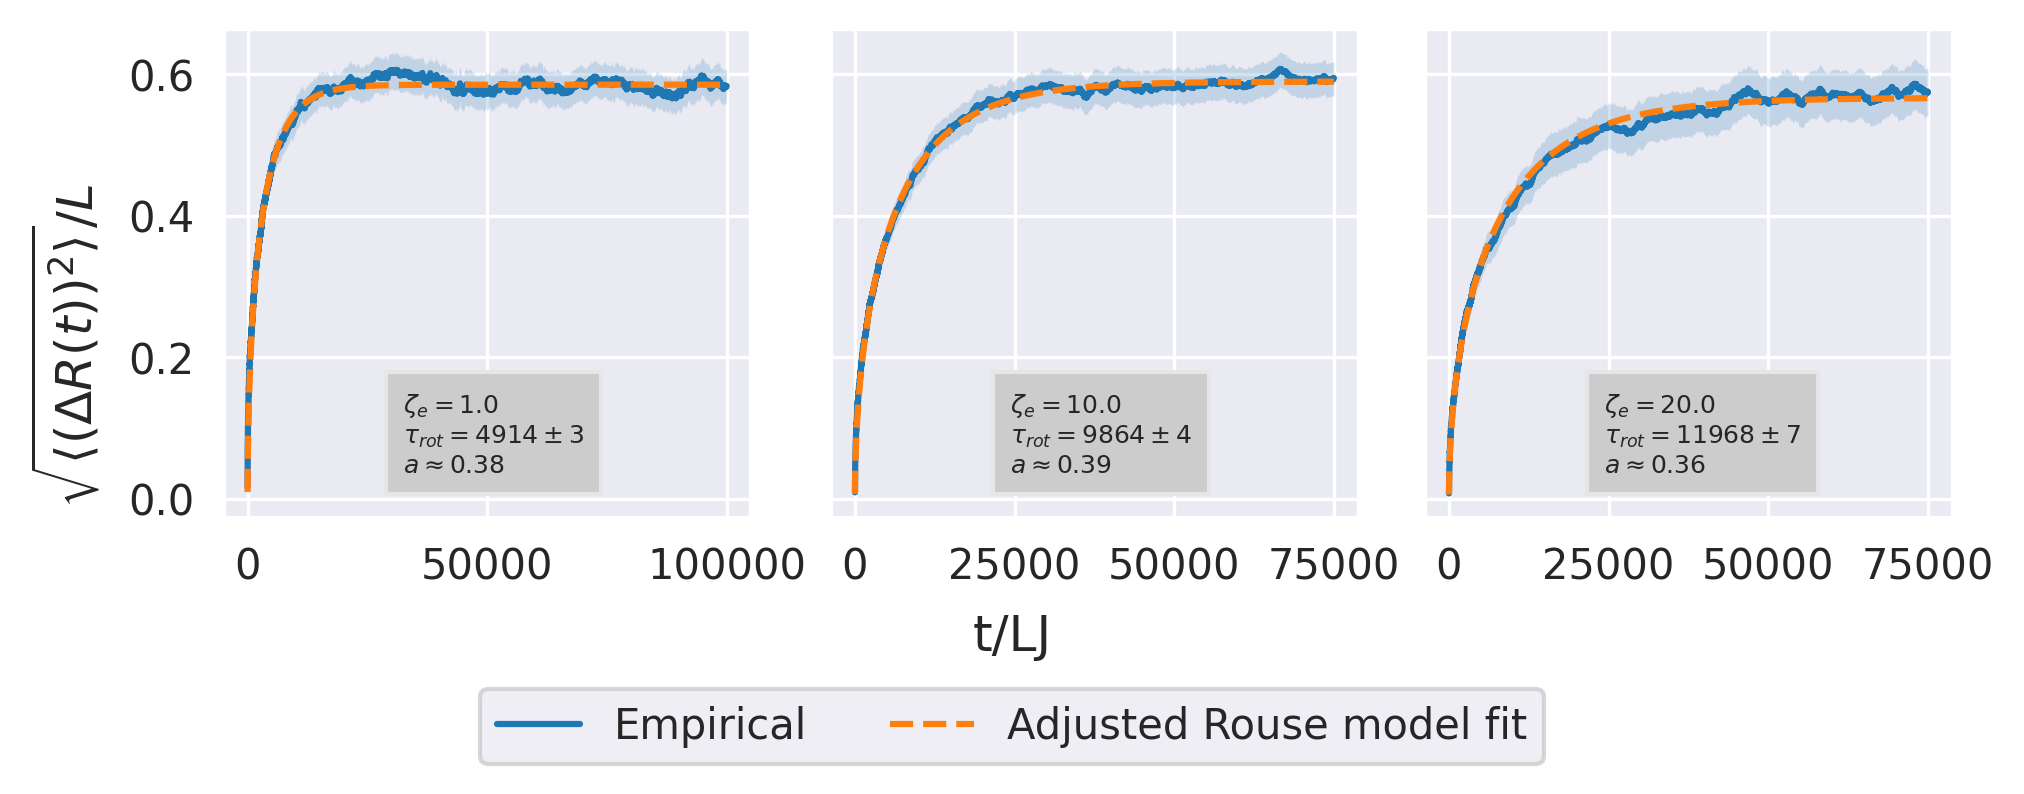
\includegraphics[width=\textwidth]{14+15+16-exp-msd-log-arm_fit.png}
        \caption{linear scale}
        \label{fig:msd_anchored_zeta-arm_fit-normal}
    \end{subfigure}
    \begin{subfigure}[b]{\textwidth}
        \centering
        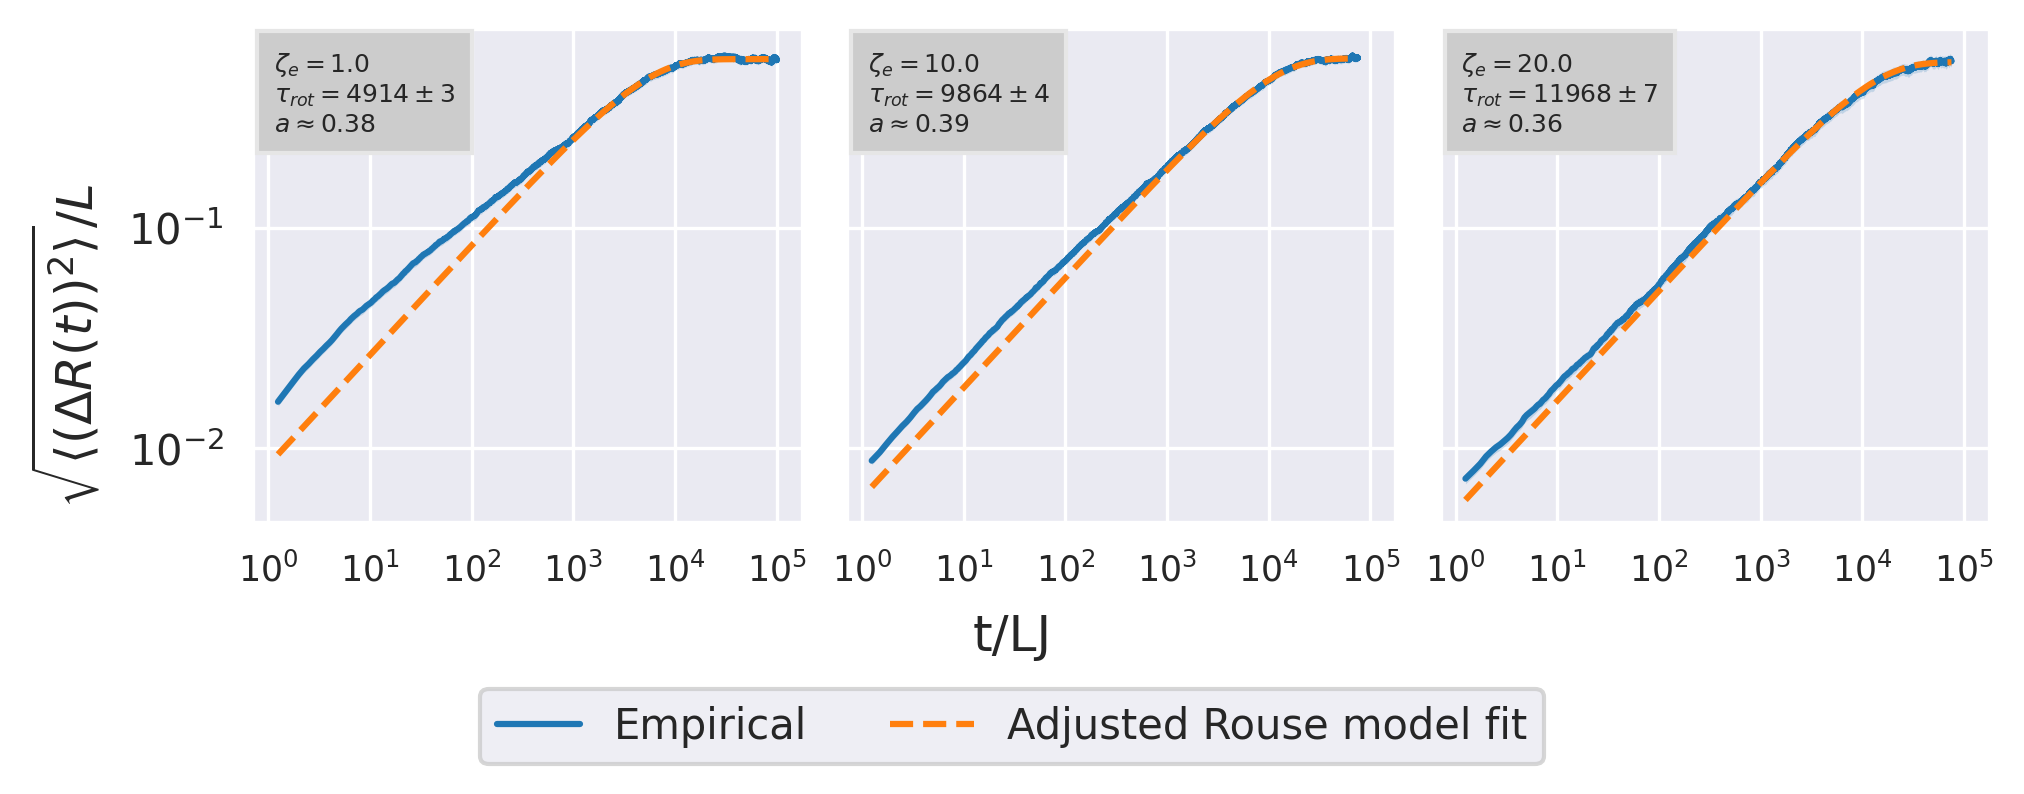
\includegraphics[width=\textwidth]{14+15+16-exp-msd-log-arm_fit-log.png}
        \caption{log-log scale}
        \label{fig:msd_anchored_zeta-arm_fit-log}
    \end{subfigure}
    \caption{Empirical MSD of ETE of anchored chains with different values of
    the friction coefficient of the chain end $\zeta_e$ and a corresponding fit
    of the Adjusted Rouse model (Eq.\ref{eq:adjusted_rouse_model_ete}).
    }
    \label{fig:msd_anchored_zeta-arm_fit}
\end{figure}

\begin{table}
    \centering
    \begin{tabular}{lrrrrrrr}
        \toprule
         & $\tau_{rot}$ & $\Delta \tau_{rot}$ & $a$ & $\Delta a$ & $m_e$ & $\alpha_m$ & $\Delta \alpha_m $\\
        $\zeta_e$ &  &  &  &  &  &  &  \\
        \midrule
        1 & 4914.250775 & 2.551632 & 0.381353 & 0.000096 & 1.0 & 0.736970 & 0.055872 \\
        10 & 9863.543716 & 3.602848 & 0.387068 & 0.000071 & 1.5 & 0.919990 & 0.067072 \\
        20 & 11967.770149 & 7.068073 & 0.357454 & 0.000103 & 1.5 & 0.928494 & 0.070997 \\
        \bottomrule
    \end{tabular}
    \caption{
        Anchored chain, $l_K/L=6.02$. 
        Estimated values of free parameters of Adjusted Rouse model (Eq.\ref{eq:adjusted_rouse_model_ete}),
        estimated scaling exponent $\alpha_m$ and corresponding $\zeta_e$ and $m_e$ values.
    }
    \label{table:anchored_chain_zeta_estimations}
\end{table}


\begin{figure}
    \centering
    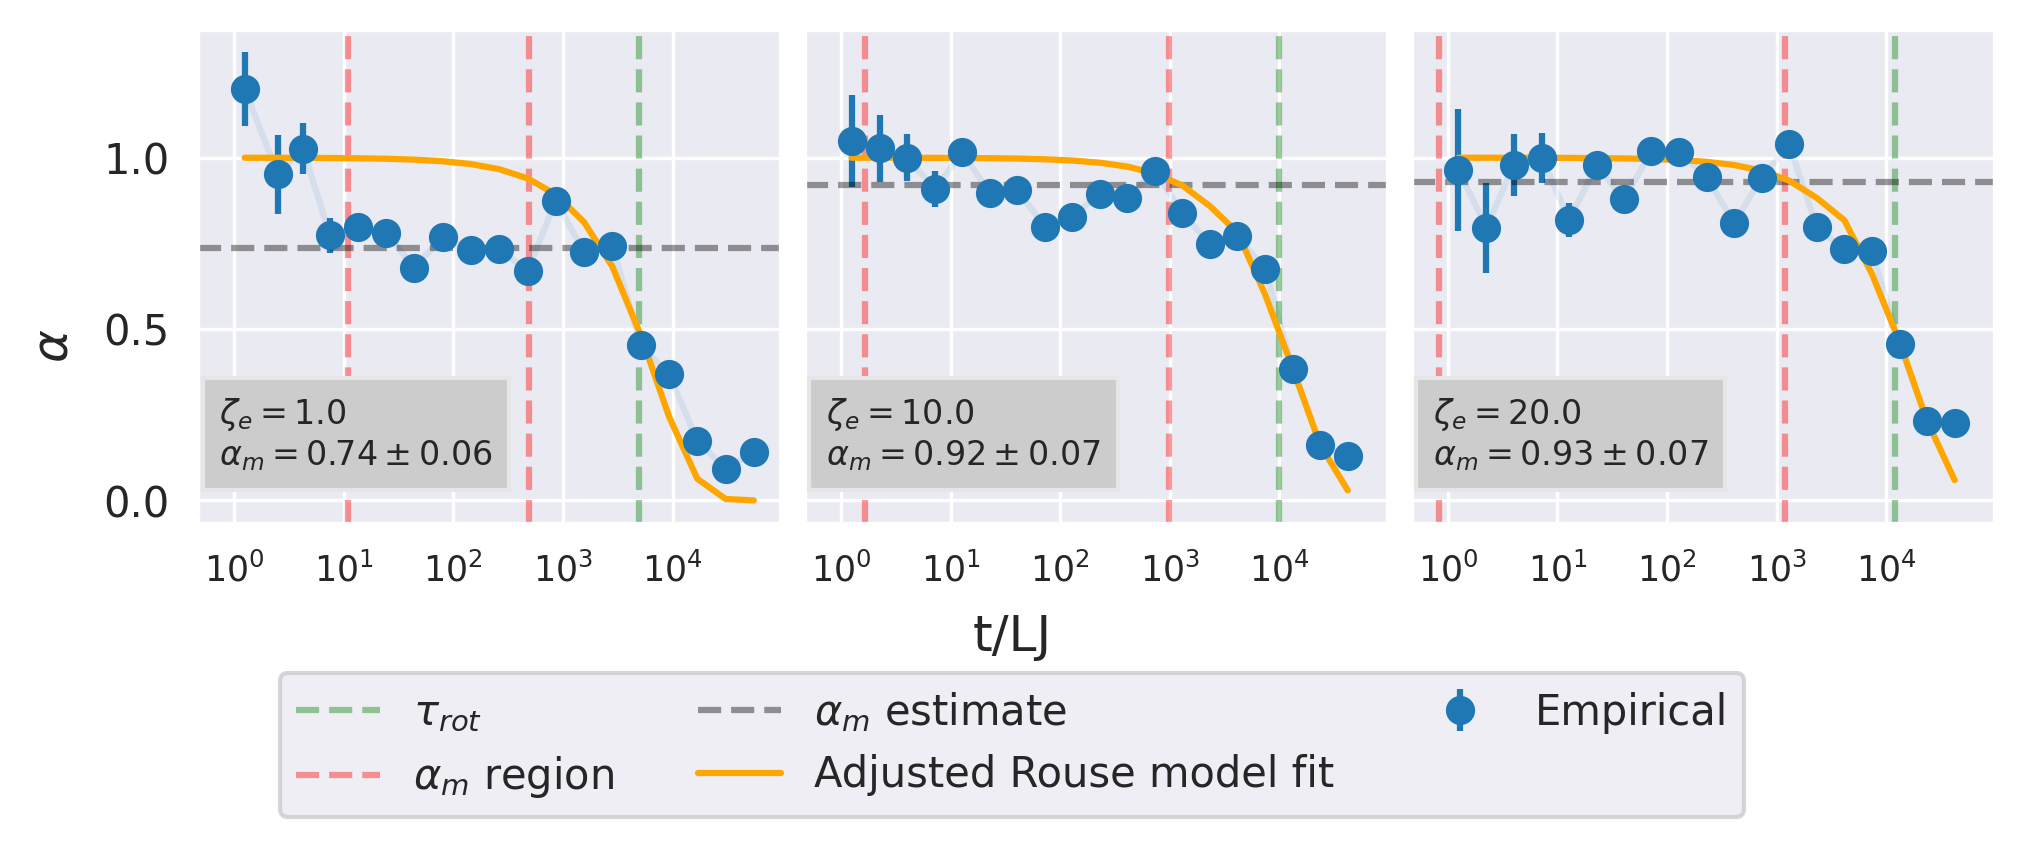
\includegraphics[width=\textwidth]{14+15+16-exp-alpha.png}
    \caption{Scaling exponent $\alpha$ of MSD of ETE 
    of anchored chains with different values of
    friction coefficient of the chain end $\zeta_e$ (blue dots).
    Scaling exponent $\alpha$ of corresponding fit 
    (section \ref{sec:impact_of_zeta_e}, 
    paragraph: Comparison with the Rouse model)
    of the adjusted Rouse model (Eq.\ref{eq:adjusted_rouse_model_ete}, 
    orange line). Estimated scaling exponent for the time interval
    $t \ll \tau_{rot}$: $\alpha_m$ (grey dashed line); Red dashed lines
    correspond to $\alpha_m$ scaling region which is estimated as:
    $[10 \frac{m_e}{\zeta_e}, \frac{\tau_{rot}}{10}]$
    }
    \label{fig:alpha_anchored_zeta}
\end{figure}

\begin{figure}
    \centering
    \begin{subfigure}[b]{\textwidth}
        \centering
        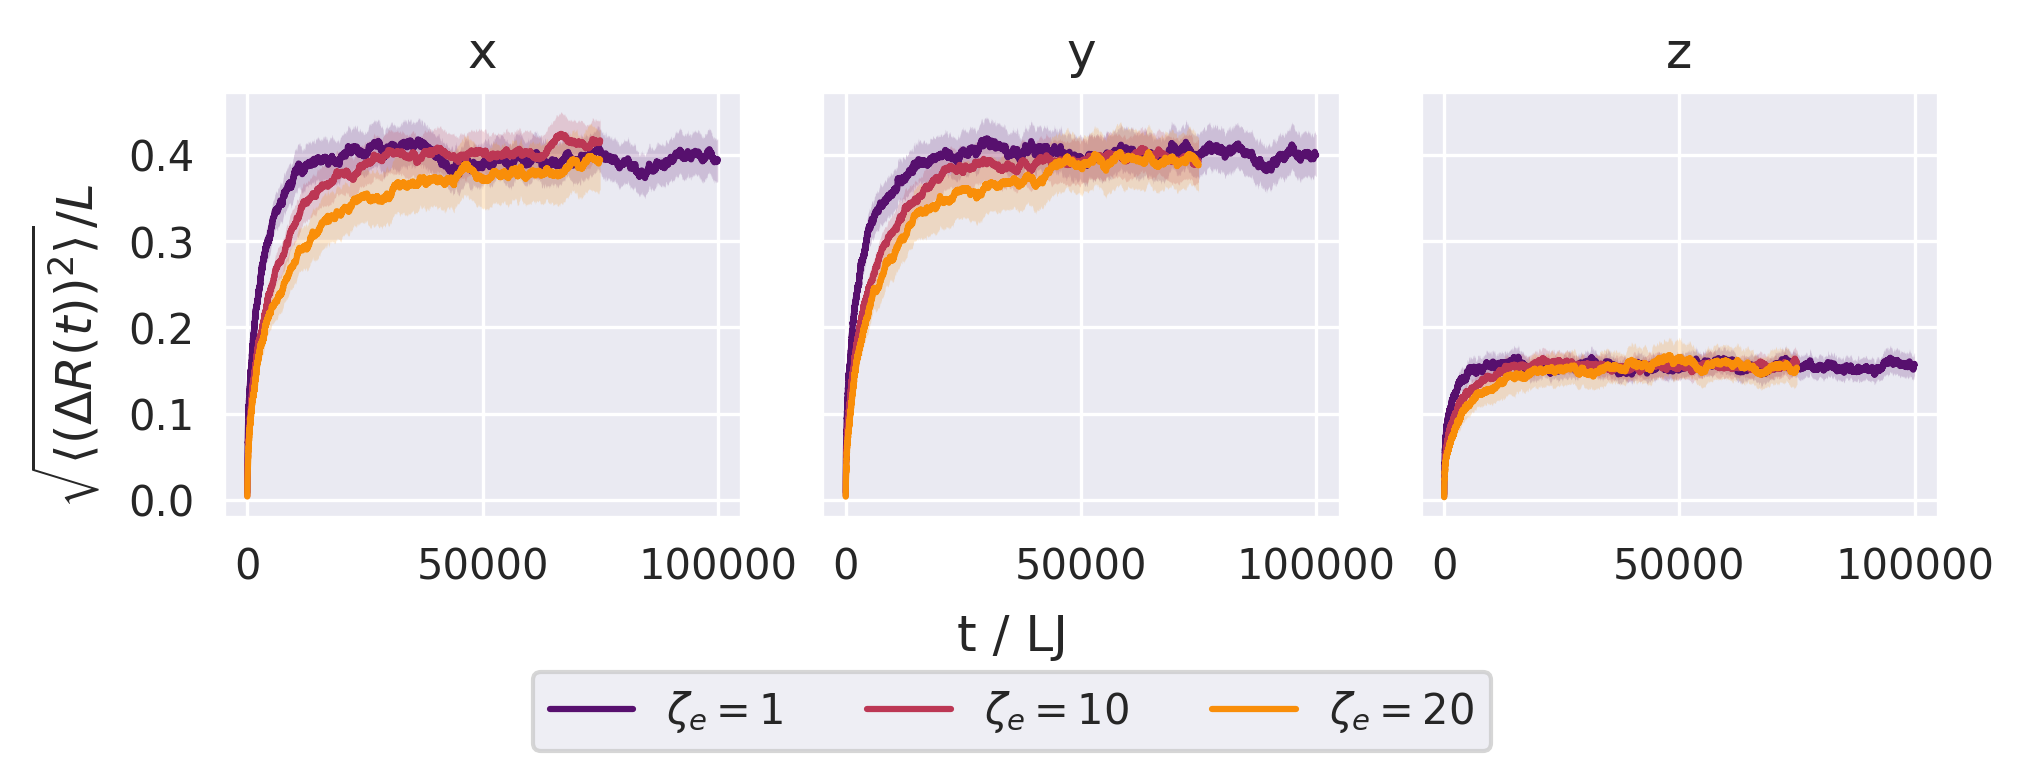
\includegraphics[width=\textwidth]{14+15+16-exp-msd-dim.png}
        \caption{linear scale}
        \label{fig:msd_anchored_zeta-dim-normal}
    \end{subfigure}
    \begin{subfigure}[b]{\textwidth}
        \centering
        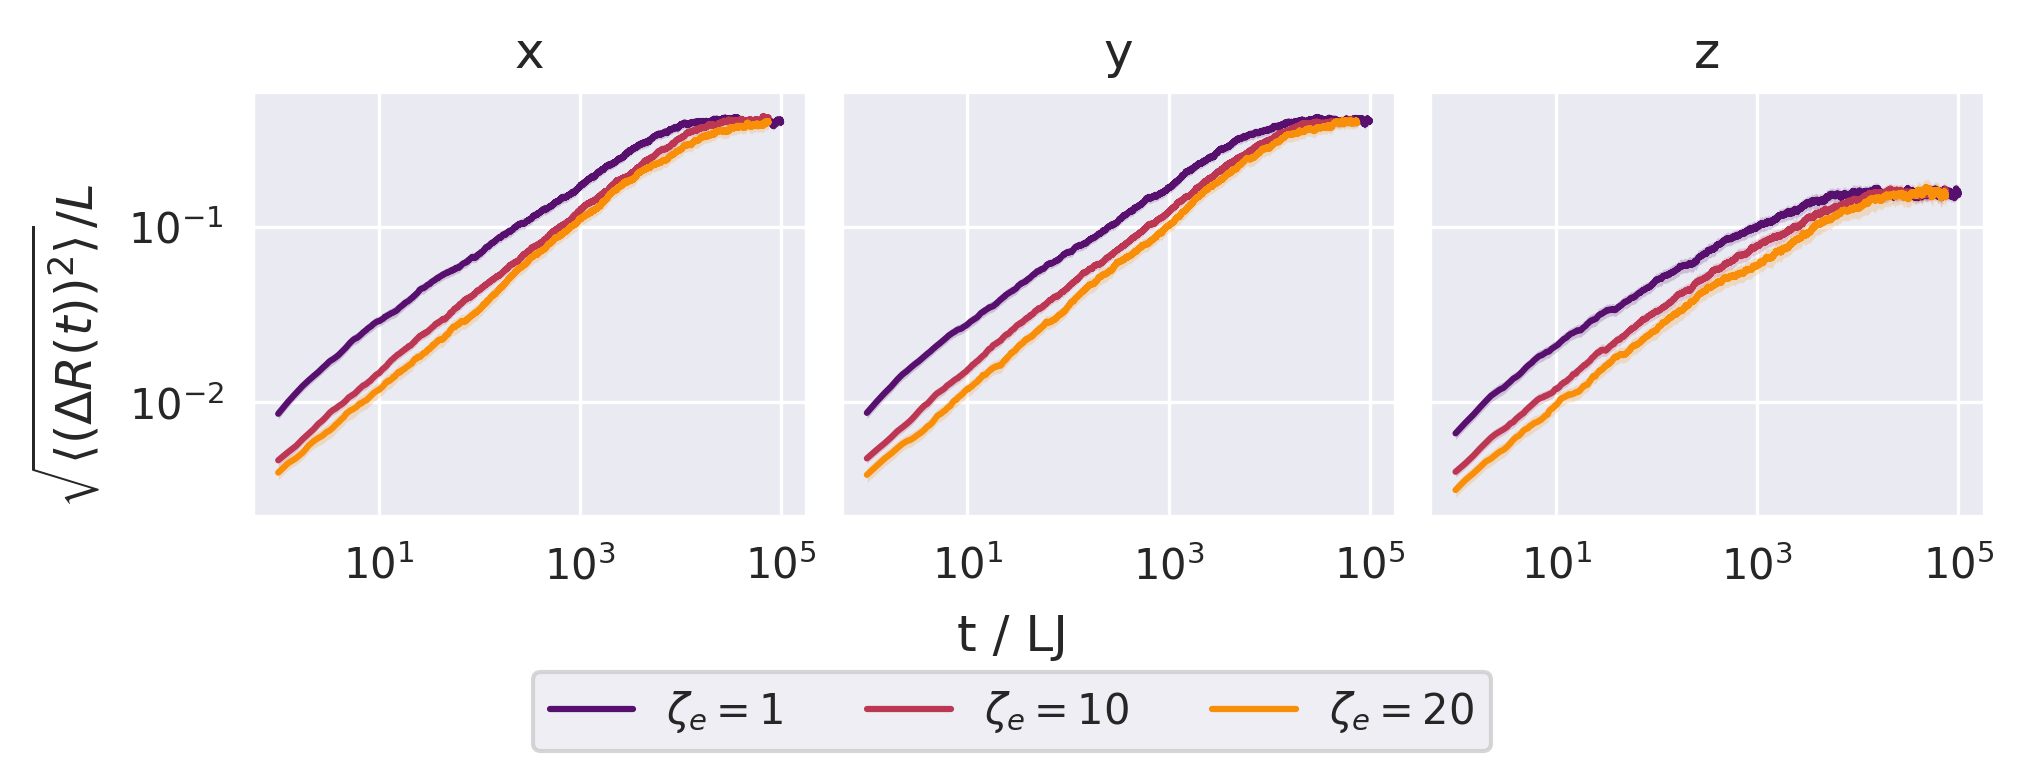
\includegraphics[width=\textwidth]{14+15+16-exp-msd-dim-log.png}
        \caption{log-log scale}
        \label{fig:msd_anchored_zeta-dim-log}
    \end{subfigure}
    \caption{
        Empirical MSD of ETE of anchored chains with different values of
        the friction coefficient of the chain end $\zeta_e$ in main-axis system
        by dimension.
    }
    \label{fig:msd_anchored_zeta-dim}
\end{figure}

\paragraph{Summary}
To summarize the findings of Section \ref{sec:impact_of_chain_stiffness}, we note:
A higher friction of the chain end slows down the overall dynamics of the chain and leads
to a delayed plateau phase. The expected (Eq. \ref{eq:autocorr_ete_rod_limit}) 
proportionality for longer time scales
$\E{\vec{R}(t)\vec{R}(0)} \propto \exp\left(-\frac{t}{\tau_{rot}}\right)$
holds for $t > \tau_{rot}$, however estimated $\tau_{rot}$ have different value and
eventually meaning than the analytical one (Eq. \ref{eq:tau_rot_rod_limit}).
Also, \autoref{fig:msd_anchored_zeta-arm_fit-log} shows, that there might be 
some analogy of characteristic time $\tau_1 < \tau_{rot}$ (Eq. \ref{eq:tau_1_rod_limit})
where above mentioned proportionality starts to be valid in analogy with Rouse model
predictions for the free semiflexible chains. On shorter timescales $t \ll \tau_{rot}$
scaling exponent $\alpha$ increases (\autoref{table:anchored_chain_zeta_estimations})
when $\zeta_e$ is increased from 1.0 to 10.0 and is not in agreement with 
Rouse model predictions for free semiflexible chains (section \ref{sec:rouse_semiflex_chain}).
Long term limits of are not affected by the damping constant.

\FloatBarrier

\subsection{Free chain dynamics} \label{sec:free_chain_dynamicss}
The following section focuses on the study of the dynamics of the 
free polymer chains. Specifically the focus is on the verification
of the hypothesis arising from the discussion in the paper of 
Singh \emph{et. al.} \cite{Singh:2022}. Their work shows, that upon the 
binding of RAB5 to the EEA1 the scaling behavior of MSDLM shifts in 
the early time regime from $3/4$ to the $2/3$. This behavior is explained
with the change of stiffness of the EEA1 upon the binding of RAB5, because
the scaling regime of MSDLM $\alpha=3/4$ corresponds the chains in the rod limit
and the $\alpha=2/3$ to the fully flexible chains in presence of hydrodynamic 
interactions. The persistence length is estimated indirectly by 
fitting the equation of MSDLM \cite{Singh:2022} derived by 
Hinczewski \emph{et al.} \cite{Hinczewski_2009}. Therefore this approach does
not proove that a change of the scaling behavior is necessarily caused by the change
of stiffness. An other factor possibly affecting the scaling behavior
is the increased friction coefficient of the end of the chain caused by the
bonded RAB5. Hence in this section the impact of the increased friction 
coefficient of the chain end ($\zeta_e$) on the scaling behavior of MSDLM is explored.
Additionally it is checked whether by changing the chain $l_p$ from the 
esimated for EEA1 value ($l_p/L_{\text{EEA1}} \approx 3.01$ \cite{Singh:2022}) to
the estimated for EEA1+RAB5 value 
($l_p/L_{\text{EEA1+RAB5}} \approx 0.3$ \cite{Singh:2022}) causes a change of its 
scaling behavior similar to the experimentally observed change.
Some simplifications are made to reduce the computational resources
requirements and implementation complexity of simulation and analysis:
the number of beads of the chain is set to $N_b=64$ which results in a
contour length $L=61.11\text{LJ}$, which then corresponds to the contour length of EEA1,
$L_{\text{EEA1}}\approx222\text{nm}$.
\\
\\
When doing the analysis of the simulation data it is possible to 
calculate MSD of one or another
chain end. In case of the symmetric chains, where $\zeta_e=\zeta=1$, both ends should 
deliver same (within confidence interval) results. In case of asymmetric chains,
where $\zeta_e > \zeta$, the results can be different. In this study
both chain ends are analyzed. We refer to the chain end, for which $\zeta_e$ is set,
as larger chain end and to the chain end, for which $\zeta$ is never changed, as 
smaller chain end. The smaller chain end corresponds to the 
chain end measured by Singh \emph{et al.} \cite{Singh:2022}.
\\
\\
For the larger chain end the obtained MSDLM curves are shown in 
\autoref{fig:msd_free}, the estimated scaling 
behavior in \autoref{fig:alpha_free} and the 
corresponding $\alpha_{min}$ values are available in 
\autoref{table:free_chain_alpha_estimations}.
For the smaller chain end the obtained MSDLM curves are shown in 
\autoref{fig:msd_fm_free}, the estimated scaling 
behavior in \autoref{fig:alpha_fm_free} and the 
corresponding $\alpha_{min}$ values are available in 
\autoref{table:free_chain_alpha_estimations_fm}.
As a plausibility check the estimated scaling behavior of fully flexible free chains is
displayed in \autoref{fig:alpha_free_full_flex}. 
\\
\\
\paragraph{Larger chain end}
Firstly, $\alpha_{min} \approx 0.727$
in case $l_K/L=6.02$, $\zeta_e=\zeta=1$ approaches the expected value for 
the chain in the rod limit ($3/4$) 
and $\approx 0.5$ (\autoref{fig:alpha_free_full_flex}) in 
case of the fully flexible chain matches almost exactly the expected value 
($1/2$), which indicates a high reliability of the method.
\\
\\
Secondly, a drop of $\alpha_{min}$ is observed 
(from $0.727\pm0.001$ to $0.659\pm0.002$, $\Delta\approx0.068$) during the
transition from $l_K/L=6.02$ to the $l_K/L=0.6$ by $\zeta_e=\zeta=1$ 
(\autoref{fig:alpha_free}).
\\
\\
Thirdly, it is observed, that an
increase of $\zeta_e$ from $\zeta_e=\zeta=1$ to $\zeta_e=10$ causes a 
non-neglible increase of $\alpha_{min}$:
In case $l_K/L=6.02$ from $0.727 \pm 0.001$ to $0.803 \pm 0.001$, $\Delta\approx0.076$.
In case $l_K/L=0.6$ from $0.659 \pm 0.002$ to $0.775 \pm 0.001$, $\Delta\approx0.116$.
Given also the MSDLM curves in \autoref{fig:msd_free}, one can conclude,
that the change in $\zeta_e$ affects the dynamics of the chains which is reflected in
the behavior of the MSD of the larger chain end. Therefore when using the fit of 
analytical expression of MSDLM
to the empirical MSD of the larger chain end to estimate some properties of the chain, 
one needs to account for the increased $\zeta_e$ to obtain more precise estimates.

\begin{table}[H]
    \centering
    
    \begin{tabular}{rrlllrrr}
        \toprule
        $\zeta_e$ & $l_K/L$ & $\tau_1$ & $\tau_b$ & $\tau_0$ & $\alpha_{min}$ & $\Delta \alpha_{min}$ \\
        \midrule
        1 & 6.02 & 78162.53 & 11.00 & 0.94 & 0.727 & 0.001\\
        10 & 6.02 & 781625.32 & 1.65 & 9.41 & 0.803 & 0.001\\
        1 & 0.6 & 6352.27 & 11.00 & 0.94 & 0.659 & 0.002\\
        10 & 0.6 & 63522.69 & 1.65 & 9.41 & 0.775 & 0.001\\
        \bottomrule
        \end{tabular}
    \caption{
        Free chains with different stiffness and end-bead friction values: 
        Estimated values of the minimum of the scaling exponent $\alpha$ and
        characteristic time scales. The larger chain end is measured.
    }
    \label{table:free_chain_alpha_estimations}
\end{table}

\begin{figure}[H]
    \centering
    \begin{subfigure}[b]{\textwidth}
        \centering
        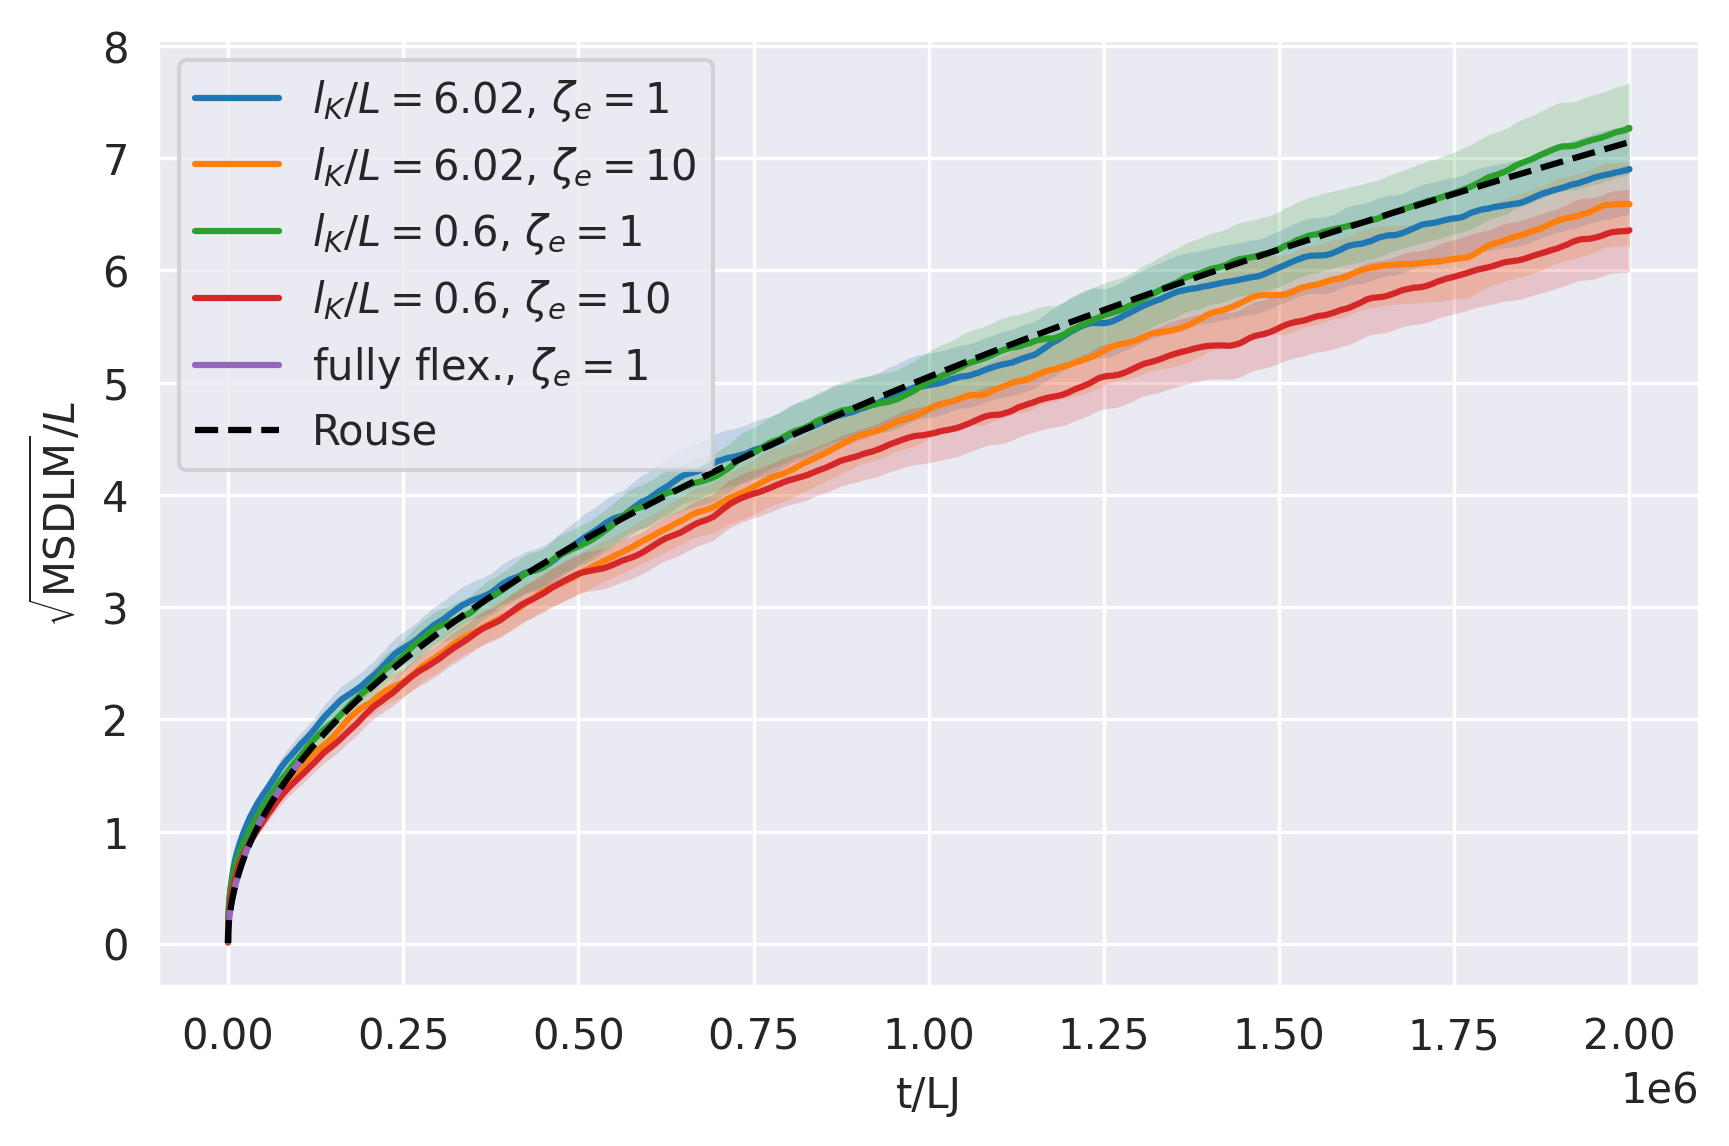
\includegraphics[width=\textwidth]{17+18+19+20-exp-msd.png}
        \caption{linear scale}
        \label{fig:msd_free-normal}
    \end{subfigure}
    \begin{subfigure}[b]{\textwidth}
        \centering
        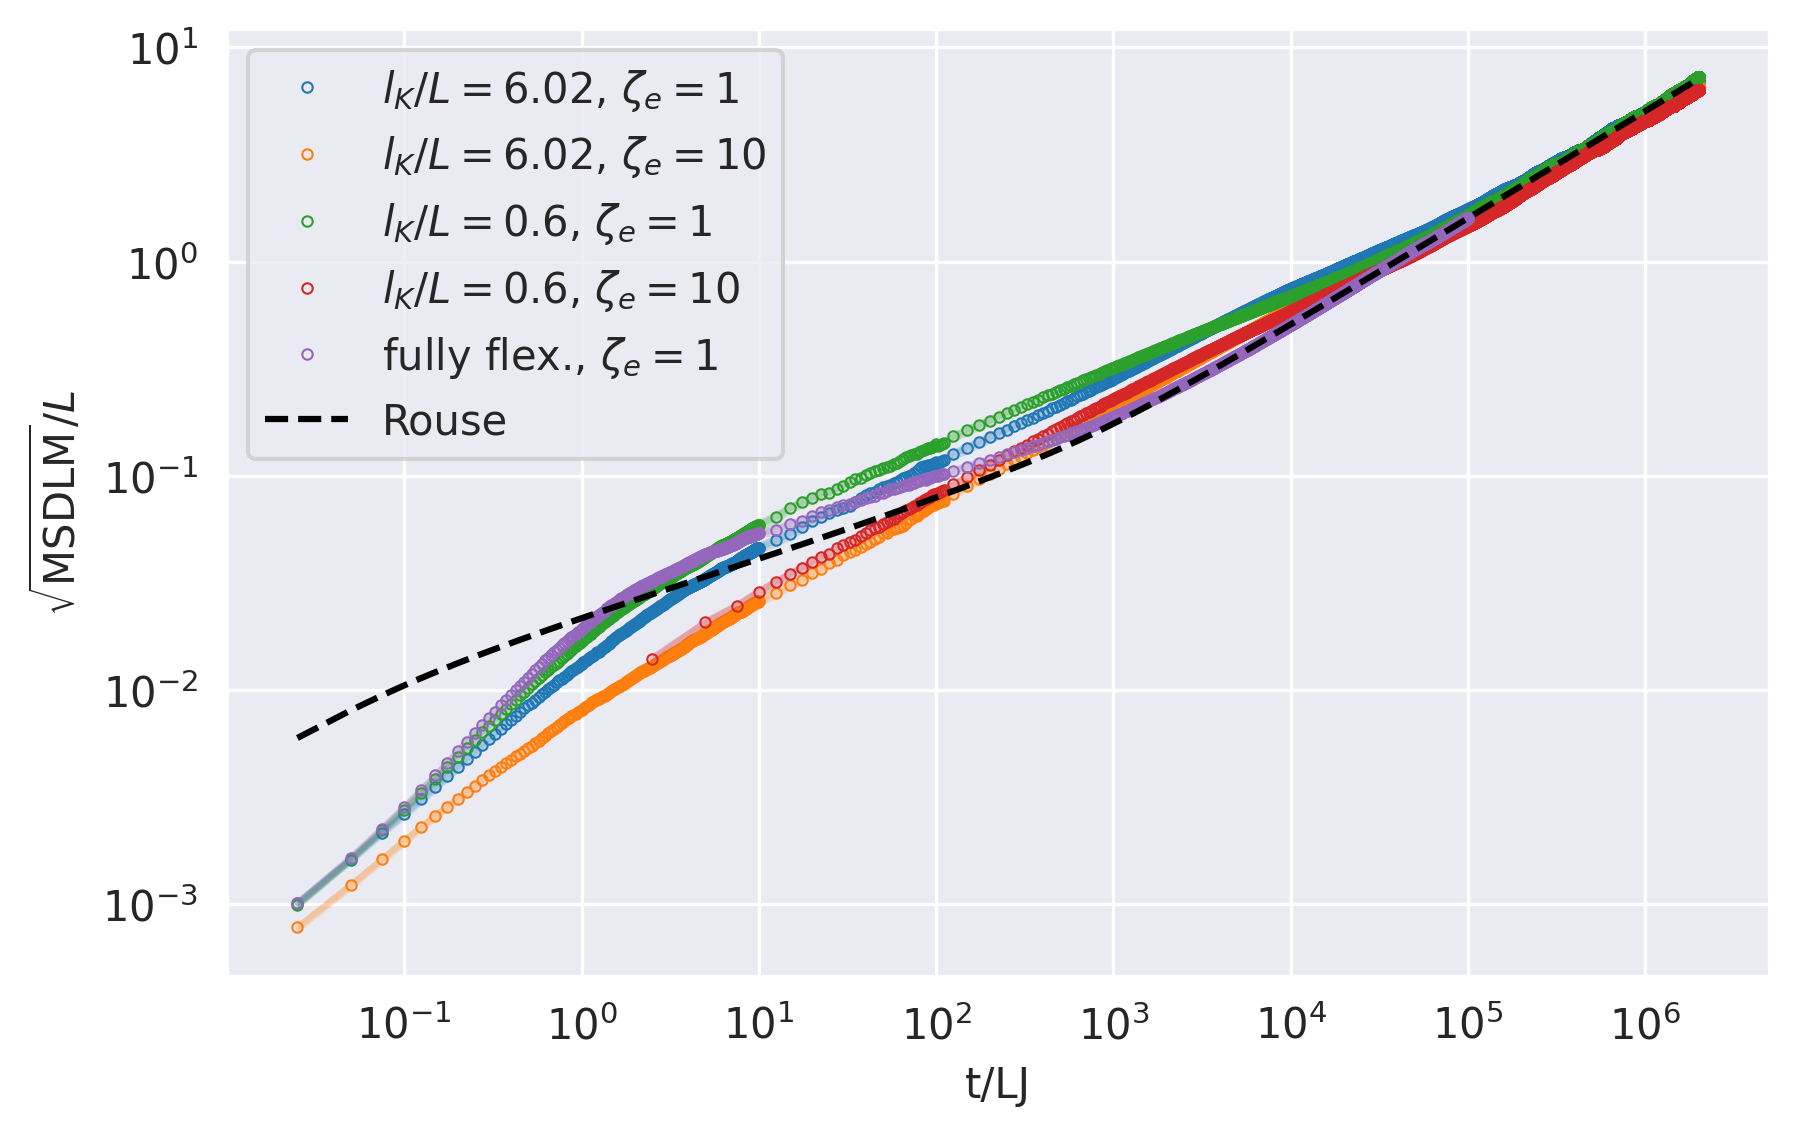
\includegraphics[width=\textwidth]{17+18+19+20-exp-msd-log.png}
        \caption{log-log scale}
        \label{fig:msd_free-log}
    \end{subfigure}
    \caption{   
        Empirical MSD of chain end (MSDLM) of free chains
        with different stiffness and end-bead friction values and
        Rouse model prediction for fully flexible chains.
        The larger end of the chain was measured.
    }
    \label{fig:msd_free}
\end{figure}

\begin{figure}[H]
    \centering
    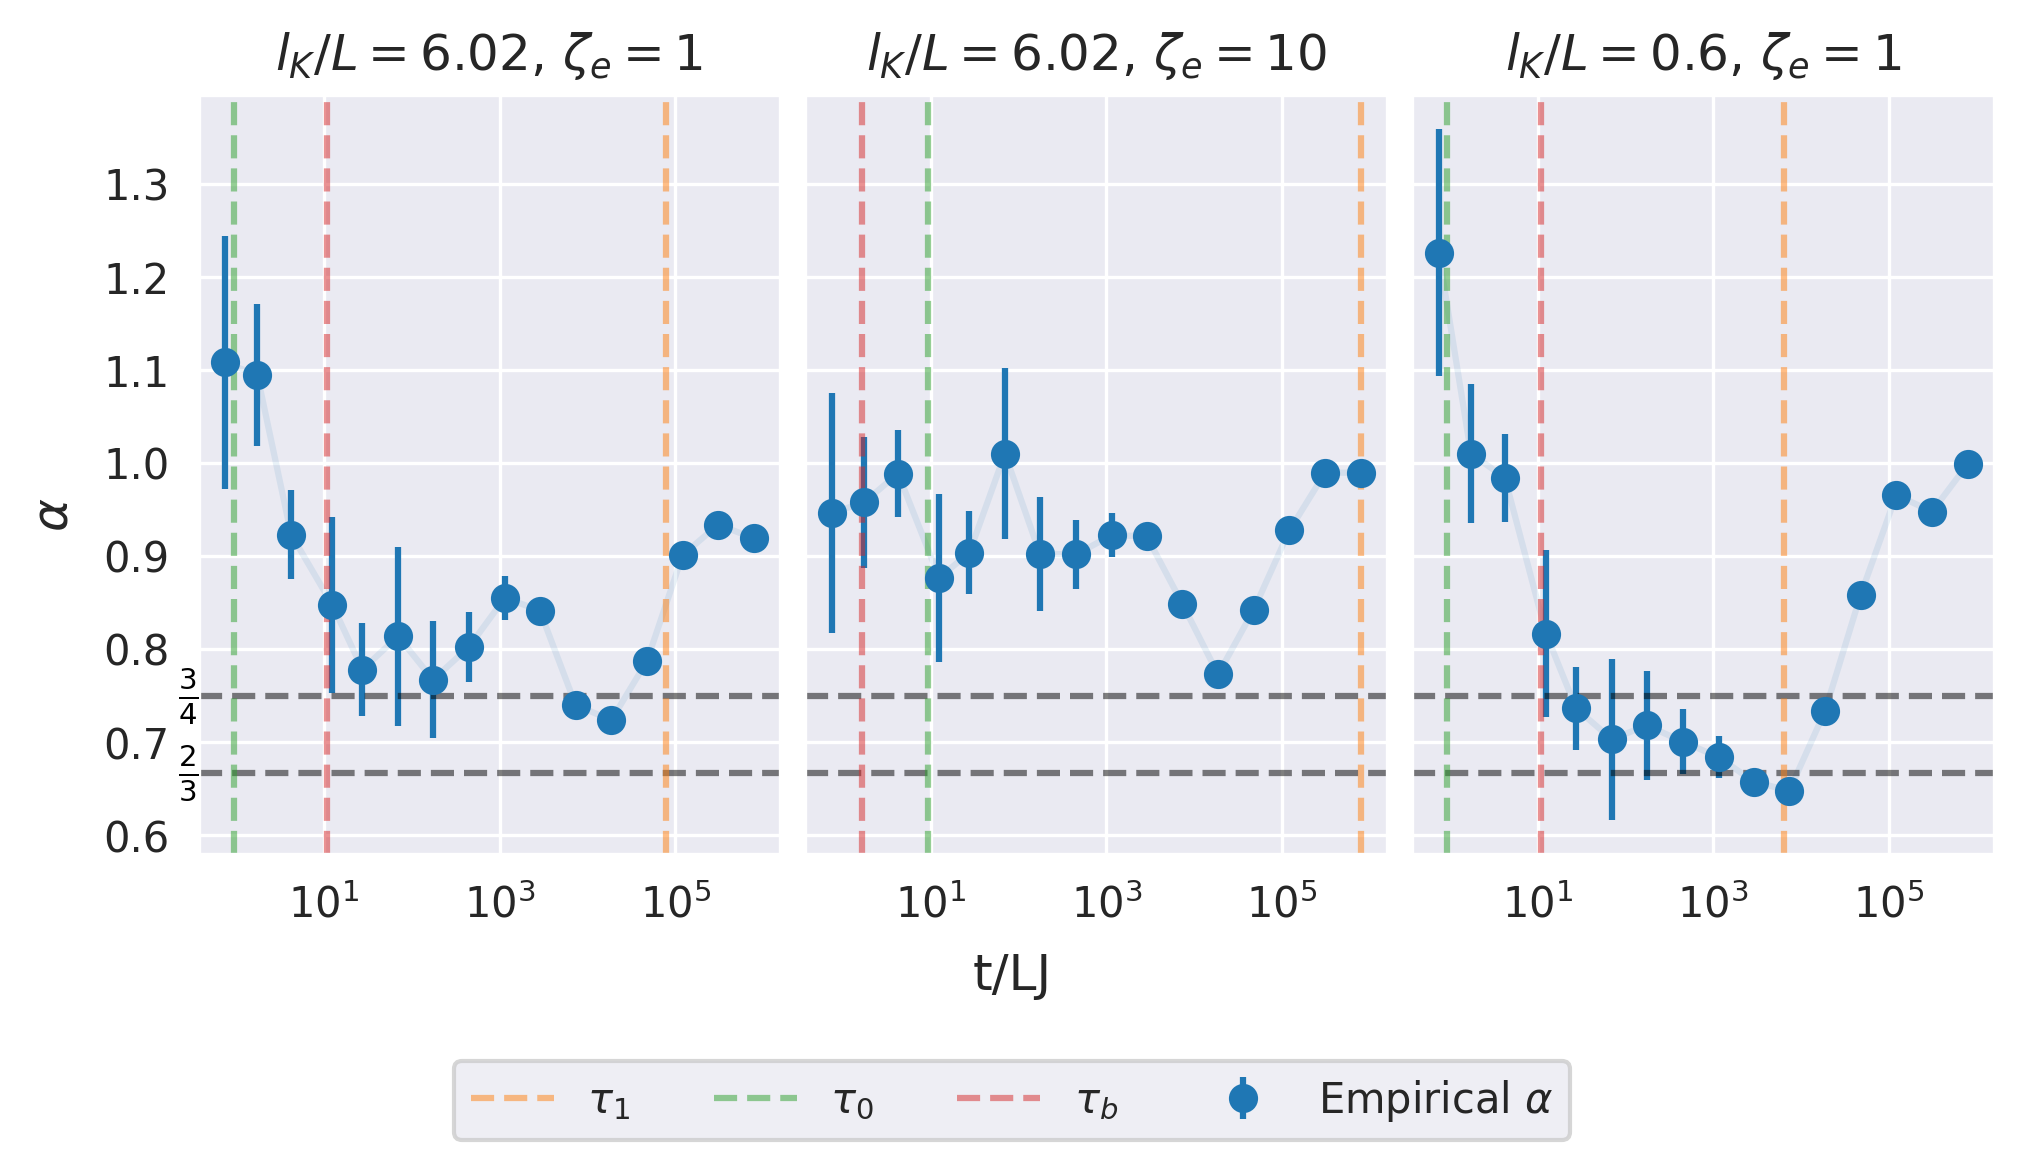
\includegraphics[width=\textwidth]{17+18+19+20-exp-alpha.png}
    \caption{Scaling exponent $\alpha$ of MSD of chain end (MSDLM) 
    of free chains with different stiffness and end-bead friction values;
    Grey dashed lines correspond to $3/4$, $2/3$, $1/2$ values.
    The larger end of the chain was measured. 
    }
    \label{fig:alpha_free}
\end{figure}

\begin{figure}[H]
    \centering
    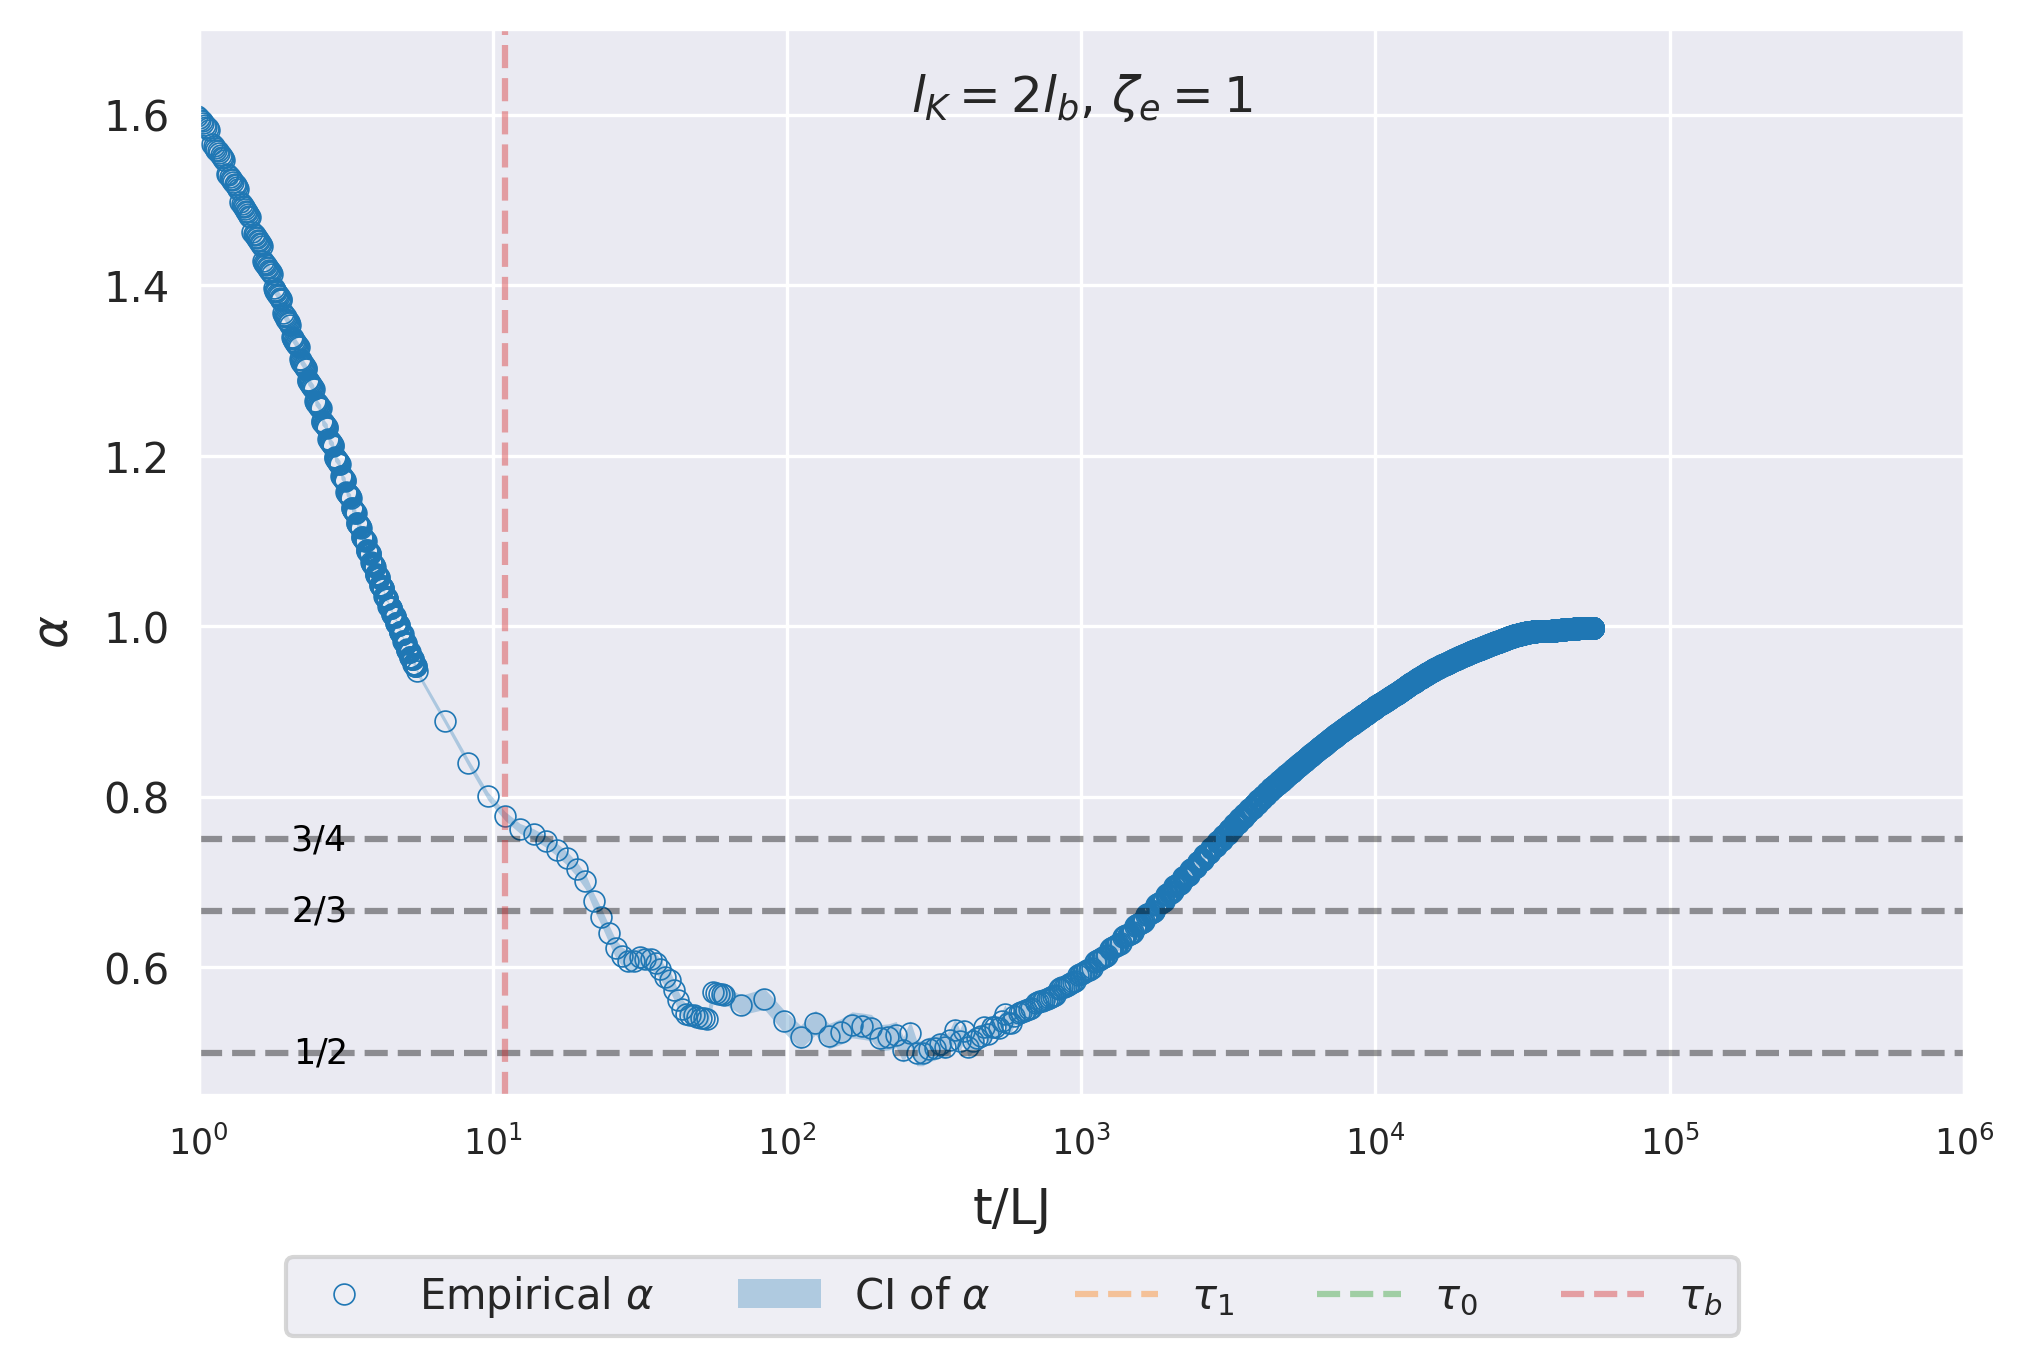
\includegraphics[width=\textwidth]{17+18+19+20-exp-full-flex-alpha.png}
    \caption{Scaling exponent $\alpha$ of MSD of chain end (MSDLM) 
    of free full flexible chain. $\tau_0$ and $\tau_b$ are outside of the
    x-axis boundaries. Estimated $\alpha_{min}=0.499 \pm 0.015$.
    }
    \label{fig:alpha_free_full_flex}
\end{figure}



\paragraph{Smaller chain end}
Firstly, we note, that the $\alpha_{min} = 0.73 \pm 0.02$
in case $l_K/L=6.02$, $\zeta_e=\zeta=1$ approaches the expected value for 
the chain in the rod limit ($3/4$) and the $\alpha_{min} = 0.652 \pm 0.002$ in case
$l_K/L=0.6$, $\zeta_e=\zeta=1$ is between $1/2$ and $3/4$ in agreement with the 
theoretical expectations. This is, similarly to the case of the larger chain end, 
an indication for the high reliability of the method.
\\
\\
\begin{figure}[H]
    \centering
    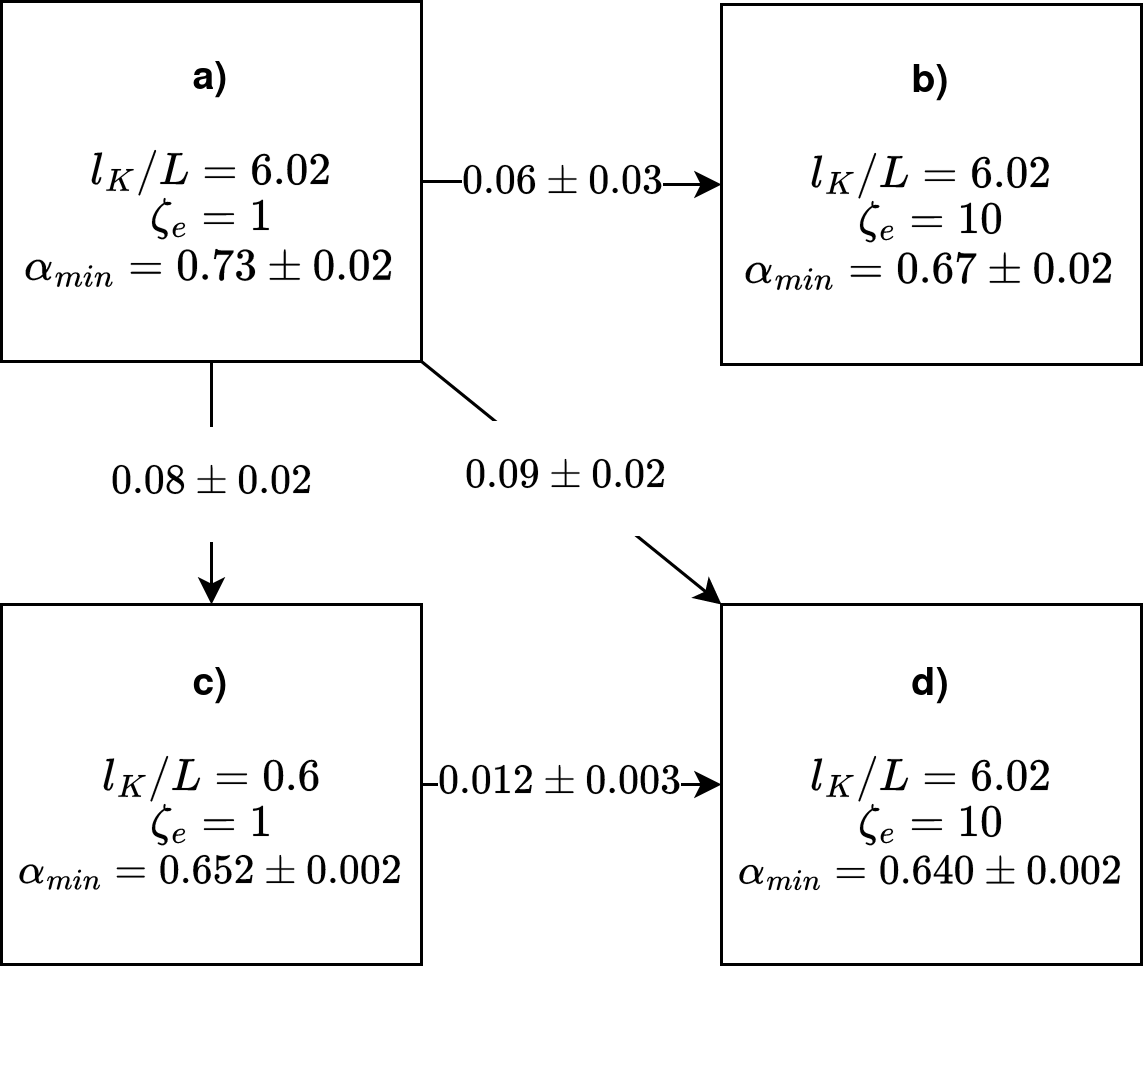
\includegraphics[width=0.48\textwidth]{cases_diag.png}
    \caption{
        Overview of cases in simulations of free chains.
        Arrows represent discussed transitions.
        A change of $\alpha_{min}$ 
        ($\Delta \alpha_{min}$, as defined in 
        Eq. \ref{eq:alpha_min_l_p_trans}, Eq. \ref{eq:alpha_min_zeta_e_trans}, 
        Eq. \ref{eq:alpha_min_l_p_zeta_e_trans}) 
        is written on the arrow.
    }
    \label{fig:alpha_cases_diag}
\end{figure}

Secondly, a drop of $\alpha_{min}$ is observed during the transition from $l_K/L=6.02$ to the $l_K/L=0.6$ by $\zeta_e=\zeta=1$ 
(\autoref{fig:alpha_fm_free}, a $\rightarrow$ c, \autoref{fig:alpha_and_delta_alpha_fm}):
\begin{equation} \label{eq:alpha_min_l_p_trans}
    \begin{aligned}
        & \alpha_{min}(a):= \alpha_{min}(l_K/L=6.02,\zeta_e=1) = 0.73\pm0.02 \\
        & \alpha_{min}(c):= \alpha_{min}(l_K/L=0.6,\zeta_e=1) = 0.652 \pm 0.002 \\
        & \Delta \alpha_{min} (a \rightarrow c) := \Delta \alpha_{min}(l_K/L=6.02,\zeta_e=1 \rightarrow l_K/L=0.6,\zeta_e=1) = 0.08 \pm 0.02
    \end{aligned}
\end{equation}  
Both values are very close 
(however the second one is outside the CI, 
which can be explained with absence of hydrodynamic and excluded volume interactions) to the ones
of Singh \emph{et al.} \cite{Singh:2022}. Moreover, $\Delta \alpha_{min} (a \rightarrow c)$
is in agreement with the change of $\alpha_{min}$ from EEA1 to EEA1+RAB5 ($\approx 0.083$)
obtained by Singh \emph{et al.} \cite{Singh:2022}.
However, in case $l_K/L=0.6$ $\alpha_{min}$ is
far larger than $\alpha_{min}$ of the fully flexible chain in contrast with the results
of Singh \emph{et al.} \cite{Singh:2022} ($\alpha_{min} \approx 3/4$ for EEA1 and 
$\alpha_{min} \approx 2/3$ for EEA1+RAB5) 
where $\alpha_{min}=2/3$ matches 
the one of the fully flexible chain, taking into account the presence of 
excluded volume interactions.
\\
\\
Thirdly, it is observed, that an
increase of $\zeta_e$ from $\zeta_e=\zeta=1$ to $\zeta_e=10$ 
(\autoref{fig:alpha_fm_free}, $a \rightarrow b$, $c \rightarrow d$) causes, in contrast
to the larger chain end, a non-neglible decrease of the $\alpha_{min}$ (\autoref{fig:alpha_and_delta_alpha_fm}):
\begin{equation}
    \begin{aligned} \label{eq:alpha_min_zeta_e_trans}
        & \alpha_{min}(b) := \alpha_{min}(l_K/L=6.02, \zeta_e=10) = 0.67 \pm 0.02 \\
        & \alpha_{min}(d) := \alpha_{min}(l_K/L=0.6, \zeta_e=10) = 0.640 \pm 0.002 \\
        & \Delta \alpha_{min}(a \rightarrow b) := \Delta \alpha_{min}(l_K/L=6.02,\zeta_e=1 \rightarrow l_K/L=6.02,\zeta_e=10) = 0.06\pm0.03\\
        & \Delta \alpha_{min}(c \rightarrow d) := \Delta \alpha_{min}(l_K/L=0.6,\zeta_e=1 \rightarrow l_K/L=0.6,\zeta_e=10) = 0.012\pm0.003
    \end{aligned}
\end{equation}
One can conclude, that a
change of the friction coefficient of the chain end affects the scaling behavior
of the MSD of the smaller chain end, decreasing corresponding scaling exponent $\alpha$ 
in the region of the subdiffusive motion. However, the influence decreases with 
decreasing stiffness of the chain. The change $\Delta \alpha_{min}(a \rightarrow b)$ is also
in agreement (within the CI) with the change of $\alpha_{min}$ by RAB5 binding to the EEA1 
($\approx 0.083$) obtained by Singh \emph{et al.} \cite{Singh:2022}.
\\
\\
Furthermore, analyzing the transition $a \rightarrow d$ (\autoref{fig:alpha_fm_free}, $a \rightarrow d$), 
which models the transition from 
EEA1 to the EEA1+RAB5, one can see the decrease of $\alpha_{min}$ (\autoref{fig:alpha_and_delta_alpha_fm}):
\begin{equation} \label{eq:alpha_min_l_p_zeta_e_trans}
    \Delta \alpha_{min}(a \rightarrow d) := \Delta \alpha_{min}(l_K/L=6.02,\zeta_e=1 \rightarrow l_K/L=0.6,\zeta_e=10) = 0.09 \pm 0.02
\end{equation}
Apart from $\alpha_{min}(d)$ being close, but outside the CI 
(which can be explained with the absence of hydrodynamic 
and excluded volume interactions), to the $\alpha_{min}$
of EEA1+RAB5, this result is qualitatively and quantitatively comptatible with the change
of $\alpha_{min}$ observed by Singl \emph{et al.} \cite{Singh:2022} 
(from $3/4$ to the $2/3$, $\Delta\approx0.083$).
\\
\\
To summarize, we have shown, that both, stiffness transition of the chain
and a 10x increase of the friction coefficient of the chain end can cause a decrease 
in the minimum of the scaling exponent $\alpha$.

\begin{figure}
    \centering
    \begin{subfigure}[b]{\textwidth}
        \centering
        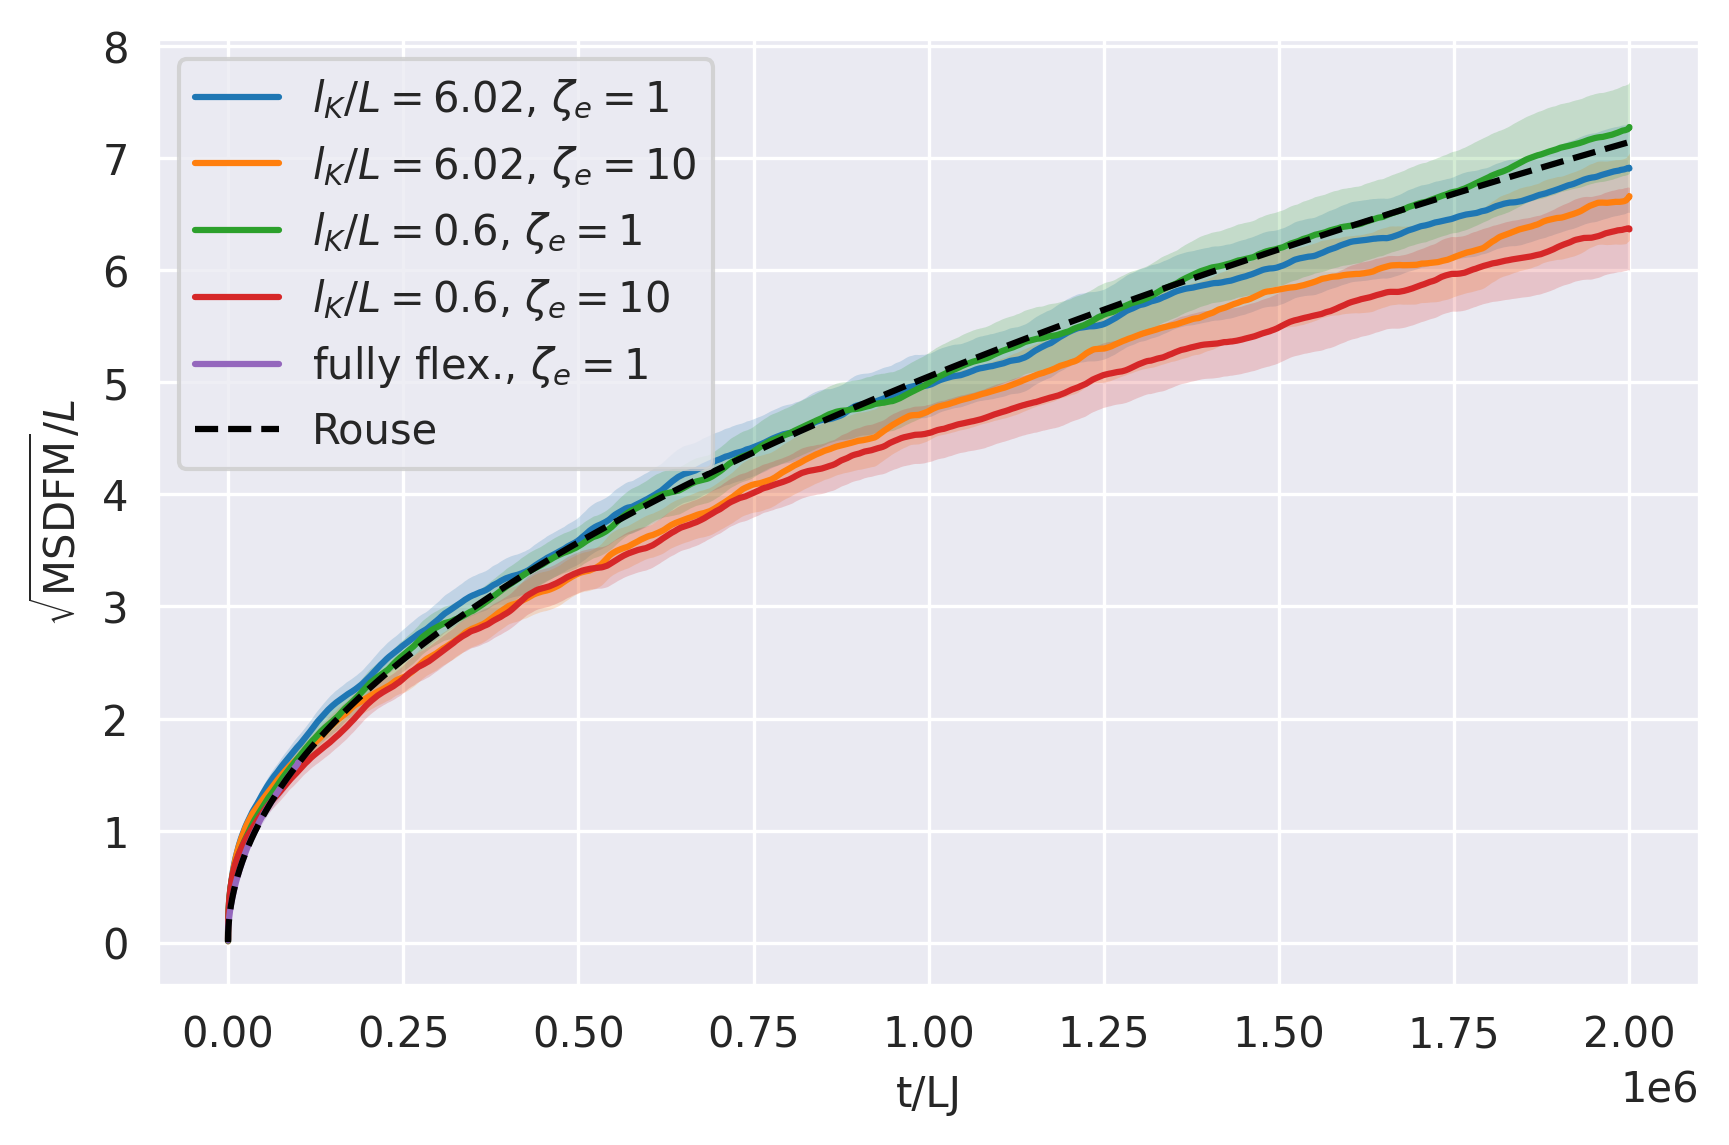
\includegraphics[width=\textwidth]{17+18+19+20-exp-msd-fm.png}
        \caption{linear scale}
        \label{fig:msd_fm_free-normal}
    \end{subfigure}
    \begin{subfigure}[b]{\textwidth}
        \centering
        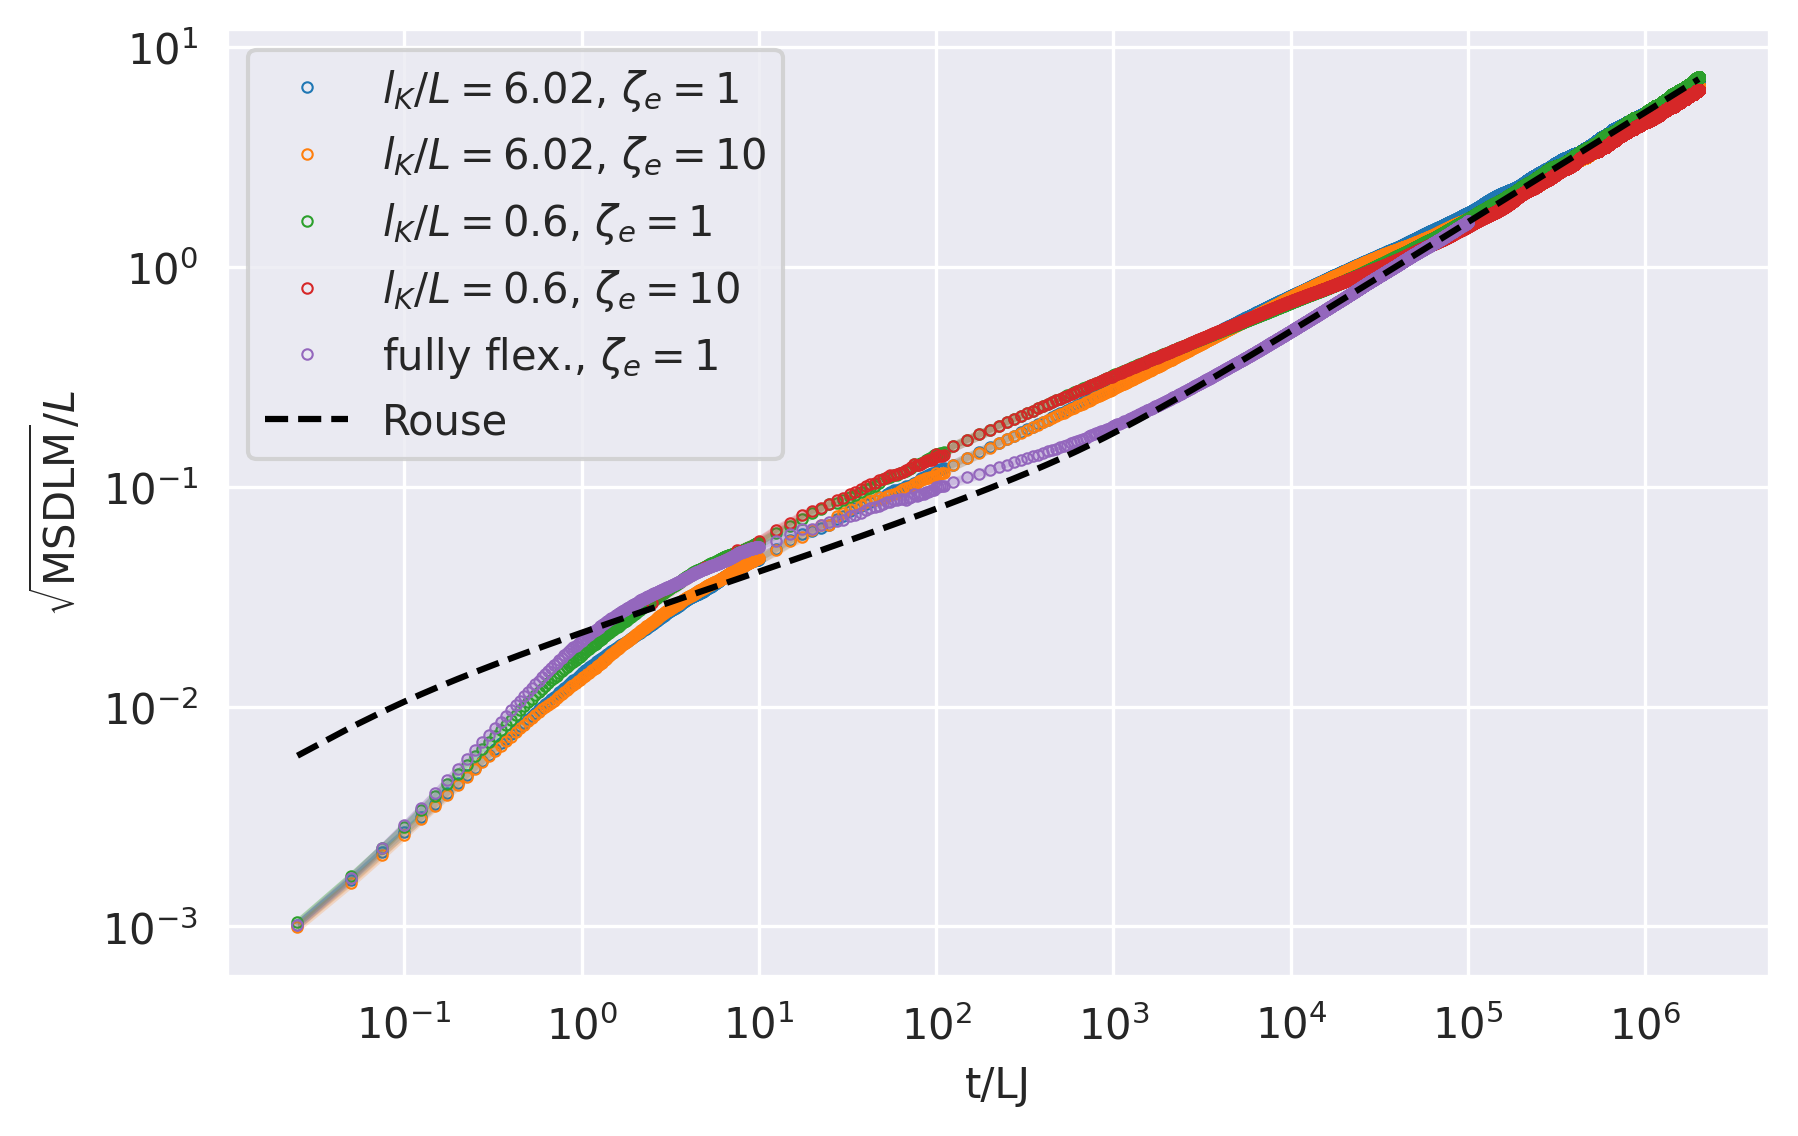
\includegraphics[width=\textwidth]{17+18+19+20-exp-msd-fm-log.png}
        \caption{log-log scale}
        \label{fig:msd_fm_free-log}
    \end{subfigure}
    \caption{
        Empirical MSD of chain end (MSDLM) of free chains
        with different stiffness and end-bead friction values and
        Rouse model prediction for fully flexible chains.
        The smaller end of the chain was measured.
    }
    \label{fig:msd_fm_free}
\end{figure}

\begin{figure}
    \centering
    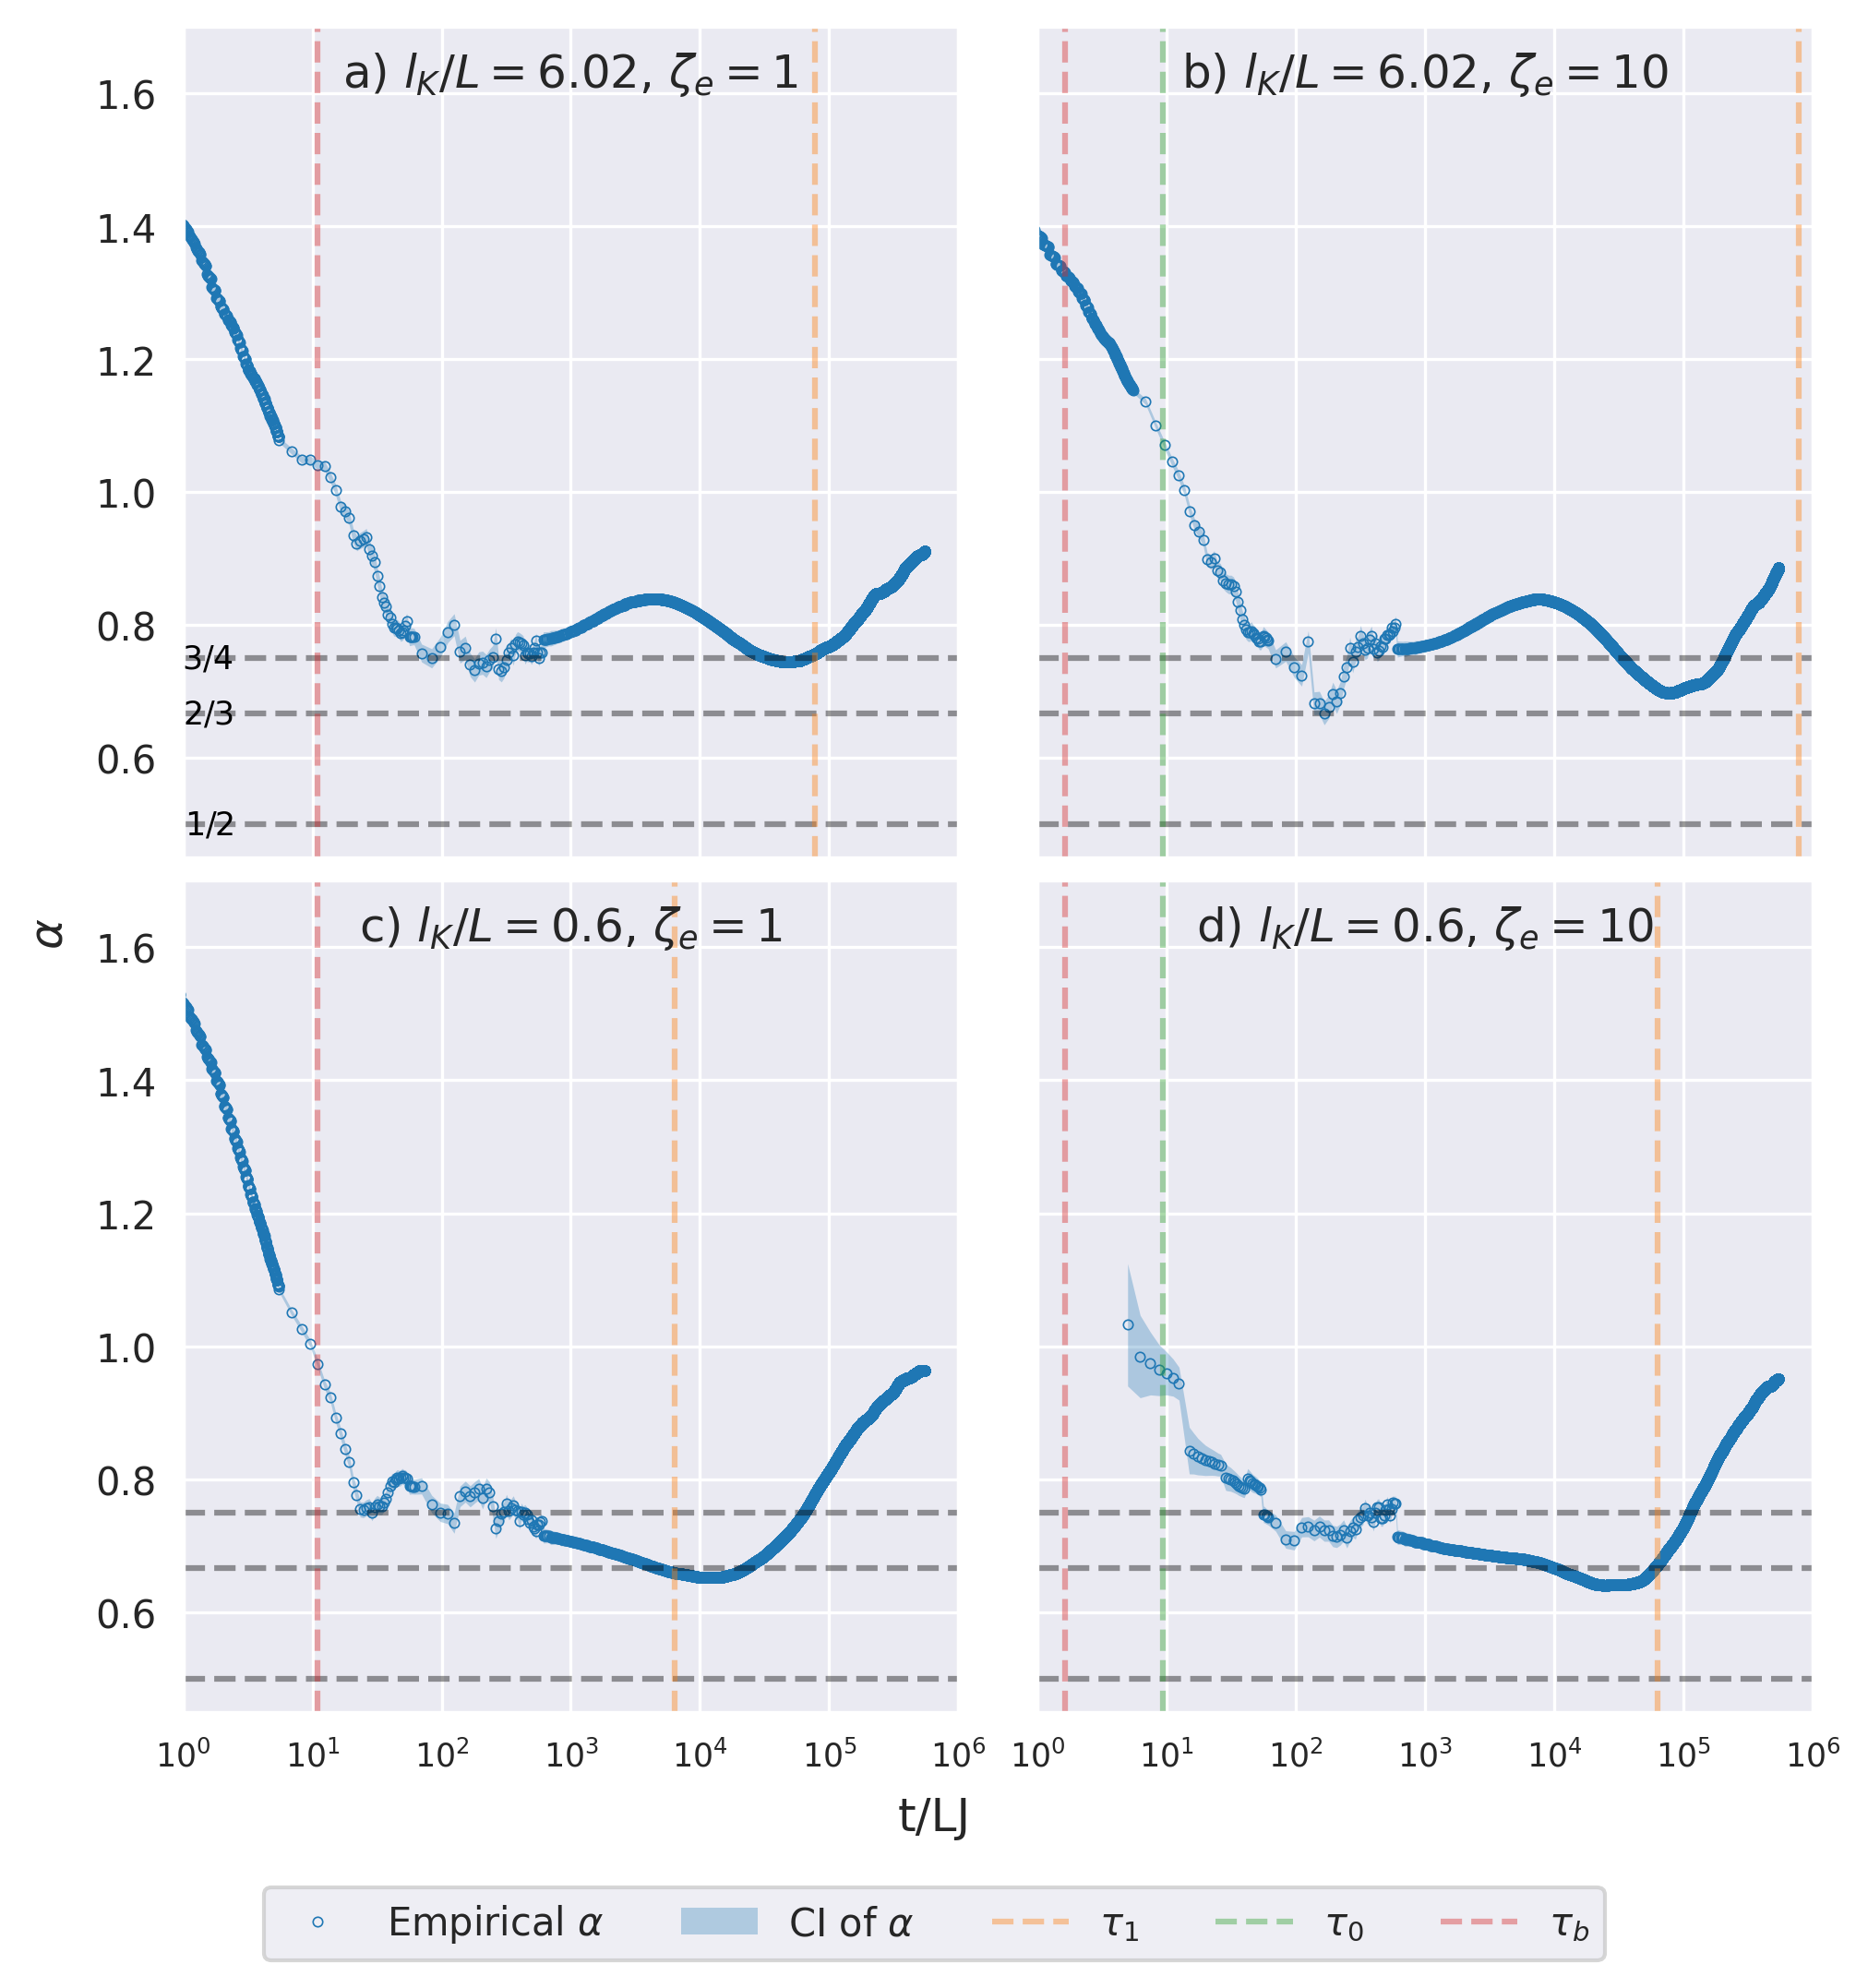
\includegraphics[width=\textwidth]{17+18+19+20-exp-alpha-fm.png}
    \caption{Scaling exponent $\alpha$ of MSD of chain end (MSDLM) 
    of free chains with different stiffness and end-bead friction values;
    Grey dashed lines correspond to $3/4$, $2/3$, $1/2$ values.
    The smaller end of the chain was measured. 
    }
    \label{fig:alpha_fm_free}
\end{figure}

\begin{figure}
    \centering
    \begin{subfigure}[b]{\textwidth}
        \centering
        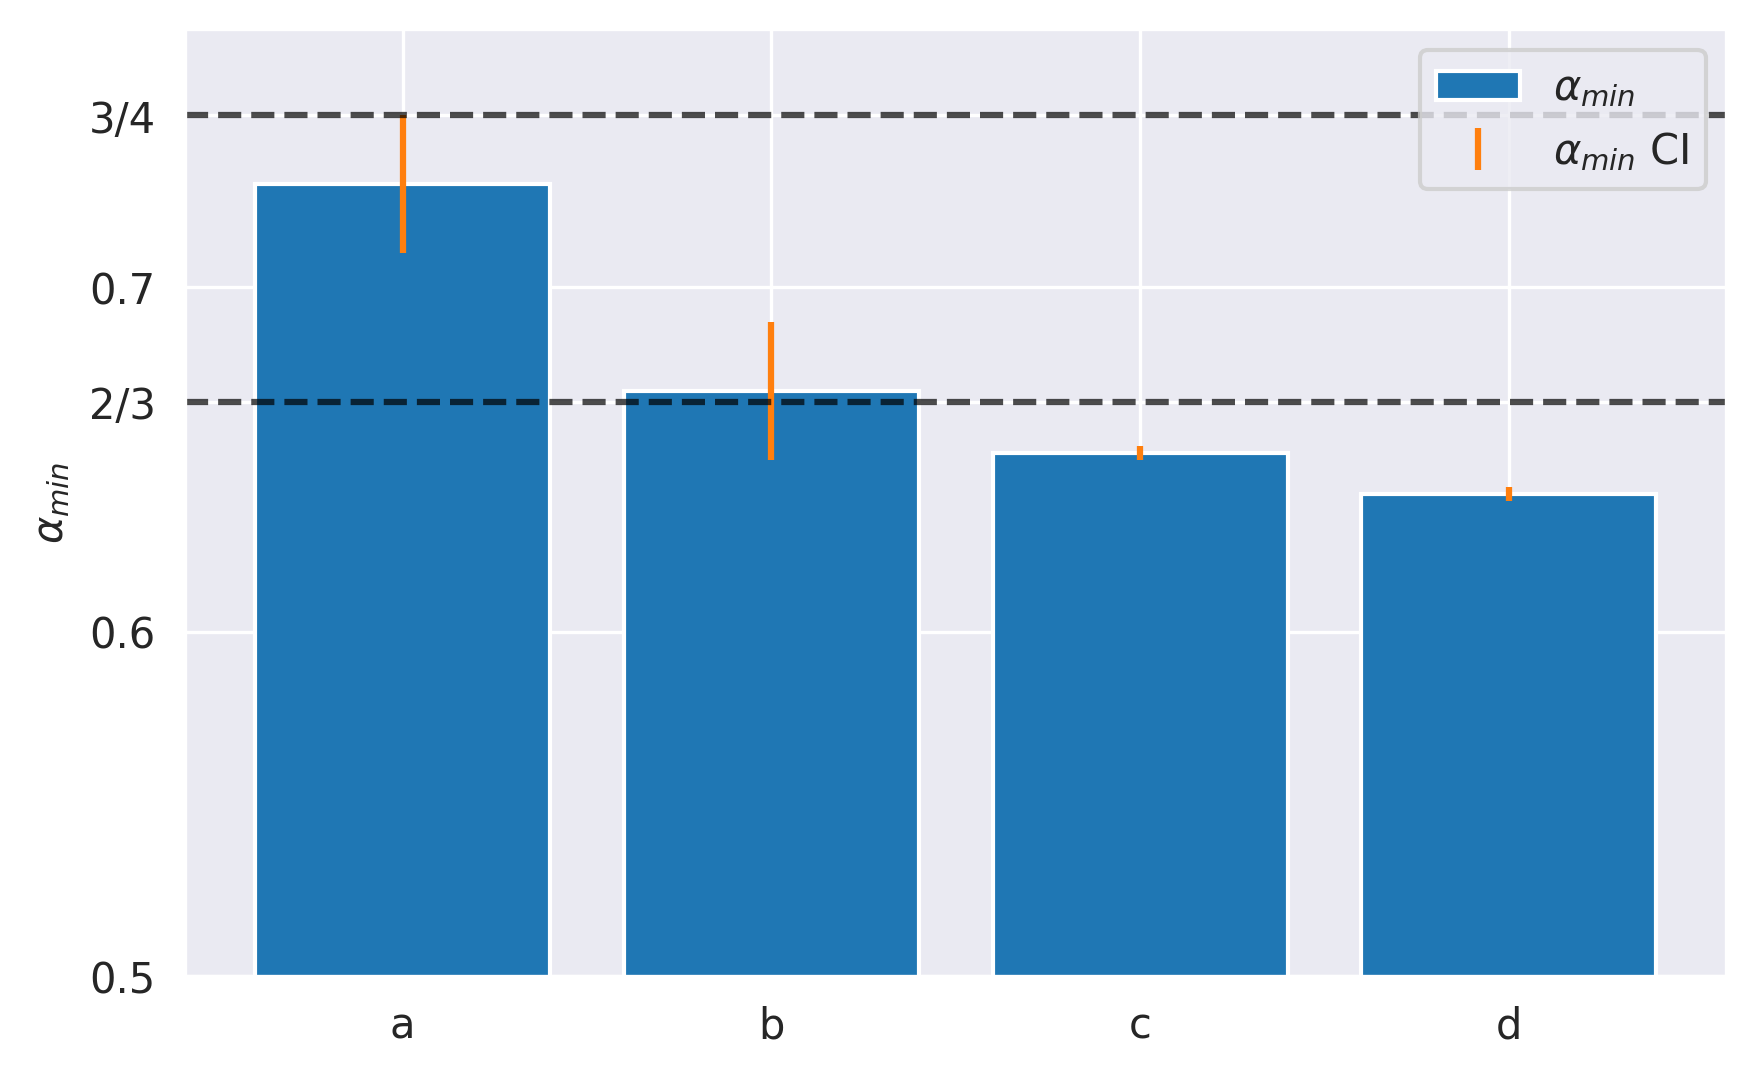
\includegraphics[width=\textwidth]{17+18+19+20-exp-alpha_min_fm.png}
        \caption{$\alpha_{min}$, smaller end of the chain}
        \label{fig:alpha_min_fm}
    \end{subfigure}
    \begin{subfigure}[b]{\textwidth}
        \centering
        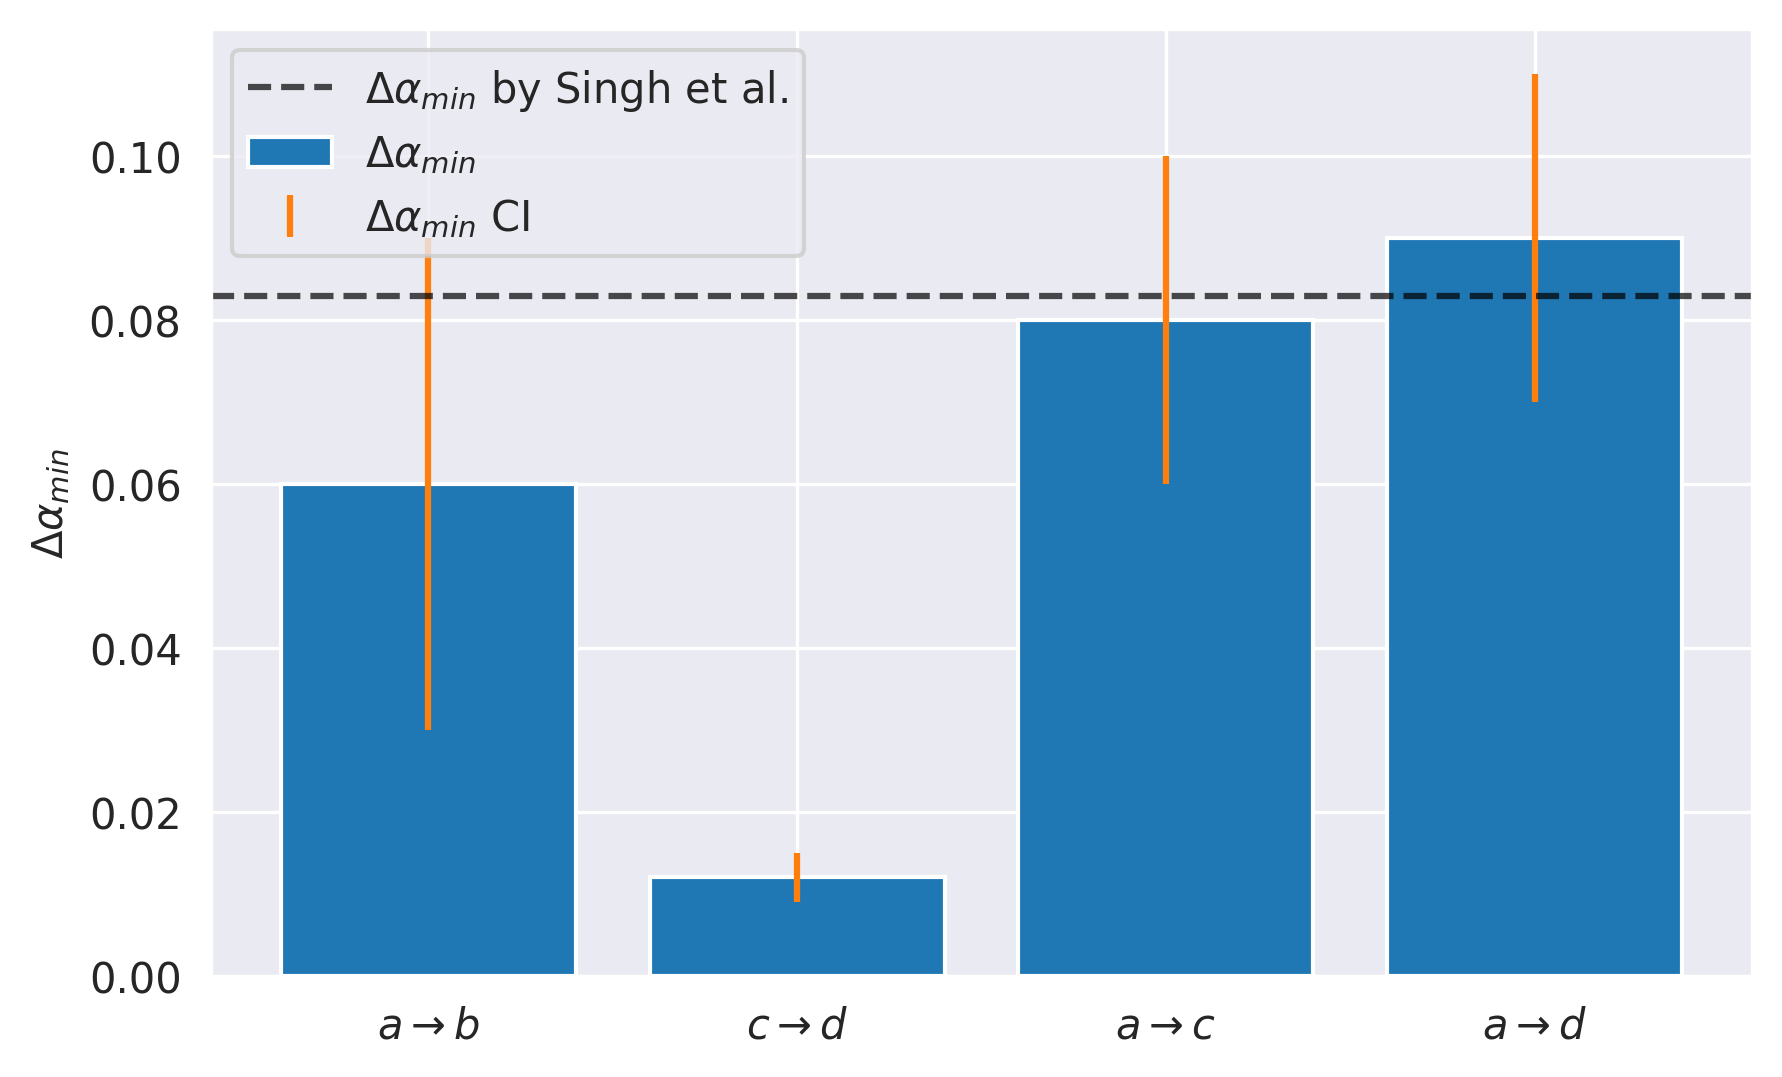
\includegraphics[width=\textwidth]{17+18+19+20-exp-delta_alpha_min_fm.png}
        \caption{$\Delta \alpha_{min}$, smaller end of the chain}
        \label{fig:delta_alpha_min_fm}
    \end{subfigure}
    \caption{
        $\alpha_{min}$ and $\Delta \alpha_{min}$ of the MSD of the smaller end of the free chain.
        Notation follows \autoref{fig:alpha_fm_free}, Eq. \ref{eq:alpha_min_l_p_trans},
        Eq. \ref{eq:alpha_min_zeta_e_trans}, Eq. \ref{eq:alpha_min_l_p_zeta_e_trans}.
    }
    \label{fig:alpha_and_delta_alpha_fm}
\end{figure}

\begin{table}[H]
    \centering
    
    \begin{tabular}{rrlllrrr}
        \toprule
        $\zeta_e$ & $l_K/L$ & $\tau_1$ & $\tau_b$ & $\tau_0$ & $\alpha_{min}$ & $\Delta \alpha_{min}$ \\
        \midrule
        1 & 6.02 & 78162.53 & 1.65 & 0.94 & 0.73 & 0.02 \\
        10 & 6.02 & 78162.53 & 1.65 & 0.94 & 0.67 & 0.02 \\
        1 & 0.6 & 6352.27 & 1.65 & 0.94 & 0.652 & 0.002 \\
        10 & 0.6 & 6352.27 & 1.65 & 0.94 & 0.640 & 0.002 \\
        \bottomrule
        \end{tabular}
    \caption{
        Free chains with different stiffness and end-bead friction values: 
        Estimated values of the minimum of the scaling exponent $\alpha$ and
        characteristic time scales. The smaller chain end is measured.
    }
    \label{table:free_chain_alpha_estimations_fm}
\end{table}

\section{Summary and Outlook}
Multiple simulations 
are performed varying the chain stiffness and friction coefficient of the chain end, 
ignoring the hydrodynamic and excluded volume interactions. 
The resulting trajectories are processed and carefully analyzed. 

\paragraph{Anchored chains}
The specific dynamical quantity, mean squared displacement 
of end-to-end distance (MSD of ETE, in following: MSD), was considered.
\\
\\
It is shown,
that the relaxation of the free fully flexible chain is faster then the relaxation of the
anchored one ($\tau_{R,\text{free}} < \tau_{R,\text{anchored}}$). 
As expected, the predictions of the Rouse model with free boundary conditions 
for the fully flexible chains do not hold for anchored fully flexible chains.
However, it is observed, that the predictions of the Rouse model with free boundary conditions 
for the fully flexible chains with $\tau_R$ as free paramater hold for anchored fully flexible
chains. The estimation of $\tau_R$ for anchored fully flexible chains 
delivers the correction factor required to account for anchoring.
\\
\\
In case of the semiflexible chain several conclusions can be made. As expected,
Rouse model predictions for flexible chains quickly deviate from observations made 
for semiflexible chains even with small stiffness ($l_p/L \approx 0.15$).
It is shown, that the MSD of anchored semiflexible chains, 
similar to the case of full flexible chains, obeys the same 
proportionality ($\propto \exp\left(-\frac{t}{\tau_{rot}}\right)$) 
as anchored semiflexible chains for longer time scales, however with
different values of characteristic time $\tau_{rot}$. These characteristic times 
$\tau_{rot}$ are estimated for different values of stiffness. It was observed, that 
$\tau_{rot}$ grows with increasing stiffness of the chain. 
To explore the shorter time
scales, the transient scaling exponent $\alpha$ of the MSD (defined in 
Section \ref{sec:est-alpha-msd}, Eq. \ref{eq:alpha_estimation_msdete}) is computed.
In the region of subdiffusive 
motion with $t\ll\tau_{rot}$ the values of the scaling exponent $\alpha$ match
qualitatively the expected minimum values of the scaling exponent of free chains.
Furthermore, the MSD was considered in a decomposition in the "main-axis" coordinate 
system (Section \ref{sec:main-axis}). It is shown, that the difference of MSD dimension parallel
to the main axis with MSD dimensions perpendicular to the main axis 
increases with growing $l_p$, specifically, the parallel dimension is 
characterized through smaller relaxation time and a lower value in the long time limit.
\\
\\
Further the impact of the friction coefficient of the chain end ($\zeta_e$) 
on the dynamical properties of semiflexible chain in the rod limit was studied.
The specific value of $l_p/L=3.01$ was selected to match the stiffness of
EEA1. Similarly to the study of impact of chain stiffness, it is shown,
that a proportionality ($\propto \exp\left(-\frac{t}{\tau_{rot}}\right)$) holds
for $t>\tau_{rot}$ if $\tau_{rot}$ is considered as a free parameter.
The increase of the estimated $\tau_{rot}$ with rising $\zeta_e$ is observed.
$\alpha(t)$ was calculated and the $\alpha$ value in the region of subdiffusive motion
(here called $\alpha_m$) was estimated. A small
increase of $\alpha_m$
($0.74 \pm 0.06 \rightarrow 0.92 \pm 0.07$) by the 
increase of $\zeta_e$ from $1$ to $10$ was observed and no difference was observed
during an increase of $\zeta_e$ from $10$ to $20$. Additionally, different projections
of the MSD were considered in the "main-axis" coordinate system, however, the effects of 
increased $\zeta_e$ are vizually shown to be consistent across the different dimensions.

\paragraph{Free chains}
The specific dynamical quantity, MSD of the chain end (in following: MSDLM), was evaluated for both 
the larger chain end and the smaller chain end (following the naming convention introduced 
in Section \ref{sec:free_chain_dynamicss}). 
The scaling exponent $\alpha(t)$ of MSDLM was examined.
\\
\\
For the larger chain end we conclude: $\alpha_{min}$ 
significantly decreases by the change from $l_p/L=3.01$ to $l_p/L=0.3$ 
in case of $\zeta=\zeta_e=1$. Both values are in agreement 
with theoretical expectations.
Furthermore it is shown, that
by increasing $\zeta_e$, the minimum of the scaling exponent $\alpha_{min}$ is also 
significantly increased in both cases: rod like $l_p/L \approx 3.01$ (matches the 
estimate for EEA1 in \cite{Singh:2022}) and
coil like  $l_p/L \approx 0.3$ (matches the estimate for EEA1+Rab5 in \cite{Singh:2022}).
Therefore, taking into account the observed MSDLM curves, the conclusion is made,
that when using the fit of analytical expression of MSDLM to the empirical MSD of
larger chain end to estimate some properties of the chain, one needs to account
for an increased $\zeta_e$ to obtain more precise estimates.
\\
\\
For the smaller chain end we conclude: $\alpha_{min}$ significantly
decreases by the stiffness decrease $a \rightarrow c$ 
(Eq. \ref{eq:alpha_min_l_p_trans}, \autoref{fig:alpha_fm_free}: $a$, $c$, 
\autoref{fig:alpha_and_delta_alpha_fm}). 
Both values are in agreement with theoretical expectations.
$\alpha_{min}(a)$ matches within the confidence interval
$\alpha_{min}$ of EEA1 obtained by Singh \emph{et al.} \cite{Singh:2022}.
$\alpha_{min}(c)$ does not match $\alpha_{min}$ of EEA1+RAB5 obtained 
by Singh \emph{et al.} \cite{Singh:2022}, which
can be explained with an absence of excluded volume and hydrodynamic interactions in the
simulation. However, the difference,
$\Delta \alpha_{min}(a \rightarrow c)$, matches
within the confidence interval the one observed by Singh \emph{et al.} \cite{Singh:2022}.
Furthermore, it is shown, that increase of the $\zeta_e$ ($a \rightarrow b$, $c \rightarrow d$) 
causes a decrease of $\alpha_{min}$ (Eq. \ref{eq:alpha_min_zeta_e_trans}, 
\autoref{fig:alpha_fm_free}, \autoref{fig:alpha_and_delta_alpha_fm}),
although this decrease is less pronounced than in the case 
of a reduction of the chain stiffness.
The difference, $\Delta \alpha_{min}(a \rightarrow b)$ 
matches, within the CI, the one observed by Singh \emph{et al.} \cite{Singh:2022}.
$\alpha_{min}(d)$ is close, however outside of the CI, 
to the one observed by Singh \emph{et al.} \cite{Singh:2022}, 
which is explained with absence of hydrodynamic
and excluded volume interactions in the simulation. 
The difference, $\Delta \alpha_{min}(a \rightarrow d)$,
is in agreement, within the CI, to the one observed by Singh \emph{et al.} \cite{Singh:2022}.
Therefore, we have shown, that both, stiffness transition of the chain
and 10x increase of friction coefficient of the chain end can cause the change
of $\alpha_{min}$, as observed by Singh \emph{et al.} \cite{Singh:2022} 
upon the binding of RAB5 to the EEA1. However, if, following the binding of RAB5 to EEA1, 
the friction coefficient at the EEA1 chain end increases by a factor of less than 10, then   
our simulations have overemphasized the effects of the larger chain end. 
Under this circumstance, it is worth noting, that 
$\Delta \alpha_{min} (a \rightarrow b)$ is much less likely 
to match the one experimentally observed by Singh \emph{et al.} \cite{Singh:2022},  
than $\Delta \alpha_{min} (a \rightarrow c)$ (see \autoref{fig:alpha_and_delta_alpha_fm}). 
Therefore, we hypothesize, that an
increase of $\zeta_e$, reasonably smaller then 10, 
would not explain the change of $\alpha_{min}$ observed by
Singh \emph{et al.} \cite{Singh:2022}.



\paragraph{Outlook}
There are several limitations of this work, which can be improved in the future research.
Firstly it is necessary to increase the chain contour length $L$ to better match both the
theoretical requirement $l_b \ll L$ and the length of the EEA1 chain. Also, one needs to
consider the smaller value of $\zeta_e$ to verify our hypothesis. Then, an improvement 
would be to consider a grid of $l_p$ and $\zeta_e$ values to obtain the 
curves of characteristic times and $\alpha_{min}$ values in dependence of 
$l_p$ and $\zeta_e$. Of specific interest is the value of $\zeta_e$ which matches 
the value of real Rab5 bound to the end of EEA1. Finally, one needs to
consider hydrodynamic and excluded volume interactions, 
which may have significant impact on the dynamical properties.  


\clearpage
\bibliographystyle{abbrv}
\bibliography{sources}

% Acknowledgement
\clearpage
\thispagestyle{empty}
\minisec{Acknowledgement}\vspace*{1.5em}
First of all I would like to express my gratitude to Prof. Dr. Jens-Uwe Sommer, 
for providing me with the opportunity to write my bachelor 
thesis at the Institute Theory of Polymers, 
for all constructive feedback, for the initial assessment of my work and 
professional advice.
\\
\\
I would also like to extend my gratitude to the second assessor 
of my thesis, Prof. Dr. Arash Nikoubashman.
\\
\\
I am sincerely grateful to my supervisor, 
Dr. Holger Merlitz, for the invaluable guidance and suppor throughout this academic journey.
Specifically,
I deeply appreciate his mentorship in understanding the theoretical framework, 
his guidance in navigating LAMMPS, his professional advice
and his proofreading of my thesis.
\\
\\
A special and warm thanks to my loving wonderful wife, Zlata, for her support
during all my studies, always being there for me, being my light during the dark times.
I would like to thank my family, especially my parents (Aliaksandr and Valiantsina), 
grandparents (Anna, Leonid, Liudmila), sister (Maria) and 
parents-in-law (Vladimir and Tatjana). And, 
of course, a big thanks to my cat, Proton, for contributing
to my mental well-being.

% Erklärung
\clearpage
\thispagestyle{empty}
\minisec{Erklärung}\vspace*{1.5em}

Hiermit erkläre ich, dass ich diese Arbeit im Rahmen der Betreuung am Leibniz-Institut für Polymerforschung Dresden e. V.
ohne unzulässige Hilfe Dritter verfasst und alle Quellen als solche gekennzeichnet habe.

\vspace*{45em}

Yahor Paromau \par
Dresden, November 2023



\end{document}
